\documentclass[12pt]{article} 

% --- Margins ---
\usepackage[a4paper, margin=0.98in]{geometry} 

% --- Font and Alignment ---
\usepackage[T1]{fontenc}
\usepackage[utf8]{inputenc}
\usepackage{XCharter} 

% --- Spacing (Clean, Modern Look) ---
\usepackage{setspace}
\setstretch{1.15} % Nice, readable line spacing
\usepackage{parskip} % Adds clean spacing between paragraphs instead of indents

% --- Your Core Packages ---
\usepackage{graphicx} 
\usepackage{booktabs} 
\usepackage{caption}
\usepackage{tabularx} 
\usepackage{array} 
\usepackage[english]{babel}
\usepackage{float}
\usepackage{amsmath}
\usepackage{subcaption} 
\usepackage[export]{adjustbox} 

% --- Citations & Bibliography (Harvard Style) ---
% Using biblatex with 'authoryear' creates the Harvard style.
% 'dashed=false' ensures author names aren't replaced with dashes if they appear multiple times.
\usepackage[style=apa, backend=biber]{biblatex}

% --- Hyperlinks (Properly connected to Citations) ---
\usepackage[colorlinks=true, citecolor=blue, linkcolor=blue, urlcolor=blue]{hyperref}
% Link the bibliography database file (replace 'references.bib' with your file's name)
\addbibresource{References.bib}
\begin{document}

\begin{titlepage}
    % --- University Logo ---
    \begin{figure}
        \centering
        
\includegraphics[height=1.5cm]{RUGLogo.png}
    \end{figure}
   
    \vspace{2cm} 
    
    % --- Title & Program Block ---
    \begin{center}
        \hrulefill\\
        \vspace{0.3cm}
        {\Large \textbf{Performance evaluation of a barrier control algorithm for autonomous vehicles at intersections using CARLA simulator}}\\ 
        \vspace{0.3cm}
        \hrulefill\\
        
        \vspace{1.5cm}
        {\large BSc Industrial Engineering and Management}\\
        \vspace{0.2cm}
        {\textit{Integration Project}}\\
    \end{center}
    
    \vfill % Pushes the metadata to the bottom of the page
    
    % --- Metadata Block ---
    \begin{flushleft}
    \begin{minipage}[t]{0.45\textwidth}
        \textit{Student:}\\
        Martijn Westerhof \\
        s5148146
    \end{minipage}
    \hfill
    \begin{minipage}[t]{0.45\textwidth}
        \textit{Supervisors:}\\
        Prof. dr. B. Jayawardhana \\
        dr. Gunn K H Larsen\\
        \textit{Daily Supervisors:}\\
        S. Pei (PhD Candidate)\\
        B. Hu (Postdoctoral Researcher)
    \end{minipage}

    \vspace{1.5cm}

    % --- Date & Word Count Floor ---
    \textit{Date:} \today
    \hfill
    \textit{Word Count: 8015}
    
    \end{flushleft}
\end{titlepage}
\section*{Disclaimer}
This report has been produced in the framework of an educational program at the University of
Groningen, Netherlands, Faculty of Science and Engineering, Industrial Engineering and Management
(IEM) Curriculum. No rights may be claimed based on this report. Citations are only allowed with
explicit reference to the status of the report as a product of a student project.
\newpage
\section*{Abstract}
Current intersection management strategies rely heavily on signalized controllers despite causing delay, increased energy consumption, and road accidents. However, the emergence of autonomous vehicles (AVs) offers an opportunity for more efficient intersection management strategies, such as a communication-free distributed barrier control algorithm. This thesis evaluates how such a controller performs against a Fully Actuated System (FAS) controller at a single intersection, using the CARLA physics based simulator. The barrier and FAS controller are simulated on a closed-loop figure-eight track and compared across four traffic densities (\(N= 51,61,71,81\) vehicles) over 30 simulations under varying initial conditions. Performance is evaluated in terms of throughput, delay time, energy consumption, and safety violations. Results highlight that the barrier controller outperforms the FAS controller across all traffic densities in throughput, delay time, and energy consumption. The out performance is attributed to the forming of a steady-state platoon which allows for continuous intersection crossing without stop-and-go behavior. However, at higher traffic densities, \(N=71\) and \(N=81\), safety violations were recorded using the barrier controller, whereas the FAS controller recorded near zero violations. The violations were only recorded during the phase before the steady-state platoon was formed, which indicates that the barrier controller itself is capable of safe performance at higher traffic densities. In conclusion, the barrier controller is found to be a promising solution for intersection management for autonomous vehicles, with room  for improvement in terms of barrier parameters to ensure completely safe operation.
\newpage
\tableofcontents
\newpage
\section*{Abbreviations}

\textbf{AV}: Autonomous Vehicle \\
\textbf{V2V}: Vehicle-to-Vehicle \\
\textbf{V2N}: Vehicle-to-Network \\
\textbf{V2I}: Vehicle-to-Infrastructure\\
\textbf{V2V}: Vehicle-to-Vehicle\\
\textbf{FAS}: Fully Actuated System\\
\textbf{ILD}: Inductive Loop Detectors\\
\textbf{EMA}: Exponential Moving Average\\
\textbf{KPI}: Key Performance Indicator\\
\textbf{CI}: Confidence Interval\\




\newpage

\section{Introduction}
Intersections are critical nodes in road networks and account for a substantial share of traffic delay, energy consumption, and road accidents \parencite{farina2026v2n, el2026distributed,bui2017real}. Traditional intersection management relies heavily on signalized control, which regulates conflicting vehicle movements through traffic light cycles. Considerable research has aimed at improving the cycle logic, ranging from actuated and adaptive timing to reinforcement-based-signal control, resulting in moderate reductions in delay and energy consumption \parencite{el2026distributed, 10433940}. However, approaches remain constrained by the signalized architecture, which is not capable of handling stochastic arrivals of vehicles, leading to idle waiting time and frequent stop-and-go behavior, especially during congestion \parencite{el2026distributed}. This stop-and-go behavior is directly relevant for energy consumption of electric vehicles, since frequent acceleration and deceleration increase the power demand of electric vehicles \parencite{kamal2014vehicle,galvin2017energy}.
\\\\
The emergence of Autonomous Vehicles (AVs) offers an opportunity to address these inefficiencies, since AVs are predictable and can adapt easily to dynamic conditions, they are capable of outperforming human drivers at coordinating intersection crossings, presenting opportunities for further delay reductions and throughput increments \parencite{soltani2025communication}. These opportunities have resulted in more research on distributed intersection management strategies that either replace or adjust traditional intersection management strategies. 
\\\\
The largest share of this research is based on Vehicle-to-Vehicle (V2V) , Vehicle-to-Network (V2N), or Vehicle-to-Infrastructure (V2I) communication, which allow vehicles to share their position, speed, and negotiate a crossing sequence. \textcite{el2026distributed} optimize vehicle crossing sequences through virtual platooning based on V2V communication, achieving increased intersection throughput and reduced delay, compared to traditional intersection management strategies. In contrast, \textcite{hasibur2021application} apply a V2I and V2V approach in which traffic signals exchange real-time phase and cycle timing information with connected autonomous vehicles, enabling vehicles to adjust their current speed to pass through the intersection more efficiently and the traffic light to dynamically adjust cycle timing. Results showed a decrease in delay and improved traffic safety. On the other hand, \textcite{bifulco2022decentralized} propose a novel longitudinal control strategy that combines on-board range sensors with V2X communication, through which vehicles exchange information to estimate each other's time to the intersection. Results show a decrease in delay time, improvements in terms of safety, and increased throughput. Although, research shows promising results in terms of throughput, delay, and safety, their reliance on communication introduces practical barriers, including the need for standardized inter-vehicle hardware, and susceptibility to delays in communication \parencite{soltani2025communication,el2026distributed}. Furthermore, V2I approaches require new infrastructure at intersections, which introduce substantial costs and single points of failure \parencite{soltani2025communication}.   
\\\\
To avoid these barriers, a smaller body of research investigates communication-free approaches, in which each vehicle decides how to traverse the intersection solely on its own onboard sensors. \textcite{song2025control} show that their adaptive barrier control function is able to safely navigate an intersection, without inter-vehicle communication.  In addition, the communication-free distributed control algorithm of \textcite{soltani2025communication}, achieved throughput comparable to an actuated signalized intersection, while reducing the average delay, using only the on board sensors to measure distances and vehicle speeds.
The results make communication-free control attractive for future-deployment, as it removes dependency on communication infrastructure.
\\\\
Despite the promising results of communication-free control, development is still in its early stages and therefore the following literature gaps exist. First, most studies evaluate intersection management strategies in simplified environments, where vehicles are modeled as points with simplified vehicle dynamics, rather than physics-based simulators which use realistic vehicle dynamics. Second, most studies examine delay time, throughput, fuel consumption and safety as the relevant performance indicators, but the effect on vehicle energy consumption is rarely studied, despite being a global concern \parencite{hadjigeorgiou2022real}.
\\\\
Therefore this thesis addresses these gaps by evaluating a communication-free distributed barrier control algorithm, against a signalized intersection, which follows a Fully Actuated System (FAS), modeled based on Dutch standards \parencite{wilson2014handboek}. The barrier control algorithm utilizes zero communication between AVs, instead each  AV independently estimates its own distance and the distance of the conflicting AV to the  point of conflict, the intersection. Based on the measurements, the AV adjusts its speed to ensure both AVs do not arrive simultaneously at the conflict point. The barrier and FAS controller are modeled, simulated, and compared in CARLA, an open-source, physics-based autonomous driving simulator \parencite{dosovitskiy2017carla}, under identical conditions. Four different traffic densities are simulated across thirty simulation runs each, where each run varied in initial spawn conditions. By evaluating both control strategies in the exact same simulation environment and only varying the intersection management strategy, the difference in performance can be attributed solely to the control strategy, which is evaluated on four Key Performance Indicators (KPIs): throughput, delay time, energy consumption and safety violations.       
\\\\
Contributions to current research, are the evaluation of the barrier control algorithm in a physics-based simulator with realistic vehicle dynamics, providing a more realistic evaluation than the simplified setups used in prior research. In addition, the evaluation focuses on vehicle energy consumption instead of fuel consumption, which is rarely studied in existing literature. 
\\\\
The objective of this thesis is to evaluate the communication-free distributed barrier control algorithm against the FAS controller in terms of throughput, delay time, energy consumption, and safety violations under  varying initial conditions,  using a single-intersection in CARLA simulator. This leads to the following research question:\\
\textit{What is the performance of a barrier control algorithm for autonomous vehicles compared to a Fully Actuated System controller at a single-intersection in terms of throughput, delay time, energy consumption, and safety, based on multiple CARLA simulations under varying initial conditions?}\\
This research question is divided into the following sub-questions:
\begin{enumerate}
    \item Which system and control parameters are required for safe and stable operation of the distributed control algorithm in CARLA?
    \item What differences in throughput, delay time, energy consumption, and safety are observed between both control strategies under identical conditions?
    \item What is the effect of varying initial conditions on the performance of both control strategies?
\end{enumerate}
The remainder of this report is structured as follows: Section~\ref{System Overview} describes the barrier controller, and the FAS controller. Section~\ref{Methodology} describes the methodology, including research approach, simulation environment, experimental design and parameters, and key performance indicators, Section~\ref{Results} presents the results, which are discussed in section~\ref{Discussion}, which is then followed by the conclusion in section~\ref{Conclusion}.   
\newpage



\section{Preliminaries: Controller Design and Formulation}
\label{System Overview}
This section first describes the setup of the barrier controller, including conflict pair identification, gradient calculation, and the barrier control law. The second part describes the FAS controller, by initially establishing the layout, which forms the basis for the phase durations, after which the phase altering system is described.



\subsection{Communication-Free Distributed Barrier Controller}
\label{Barrier based vehicle controller}
The primary function of the evaluated communication-free distributed barrier control algorithm is to adjust vehicle speed, to ensure that they never arrive simultaneously at the conflict point. 

\subsubsection{Identifying Approaching Conflict Pairs}
\label{Conflict Pair Identification}
The vehicle specific speed adjustment can only be applied if the correct conflict pair is identified. Therefore, the Barrier Control algorithm identifies the conflict pair. A vehicle is considered a candidate for the conflict pair if its Geodesic distance to the conflict point is within the conflict point and the predefined approach window \(d_\text{approach}\)(m). Per conflict point, multiple arriving candidates can be present within the approach window. Therefore, the algorithm sorts the candidates based on the distance to the conflict point. From this sorted list, the vehicle with the least distance to the conflict point per side is listed as candidate 1 (c1) or candidate 2 (c2), where the index (1 or 2) corresponds to the approach side.

\subsubsection{Computing Vehicle Distance to Conflict Point}
For each of the identified candidates, \(i \in\{1,2\}\), the distance to the conflict point is calculated. For candidate i, the distance to the conflict point \(d_\text{cross,i}\)(m), is computed by subtracting the actual position \(s_\text{actual,i}\)(m) from the position of the conflict point, \(s_i\)(m), and follows equation~\ref{dcross}\begin{equation}
\label{dcross}
    d_\text{cross,i}= s_i - s_\text{actual,i}.
\end{equation}
The value of \(d_\text{cross,i}\) from both candidates is used to calculate the relative difference in approaching distance \(\Delta d\)(m) between the candidates, which follows equation~\ref{diff}\begin{equation}
\label{diff}
    \Delta d = d_\text{cross,1} - d_\text{cross,2}.
\end{equation}
If the absolute value of \(\Delta d\) falls below the barrier activation distance \(d_\text{activation}\)(m), a gradient \(\nabla\)(-) is calculated~\ref{grad}
\begin{equation}
\label{grad}
\nabla = \frac{-1}{\Delta d}.
\end{equation}
The gradient is structured to provide a positive speed correction for the candidate closest to the intersection and a similar, but negative correction for the candidate further away from the intersection.  Furthermore, \(\nabla\) is scaled to provide larger corrections for candidates arriving with a smaller gap at the conflict point, which is represented by a smaller \(\Delta d\). 

\subsubsection{Barrier Speed Correction Law}
\label{BArrier law}
If the calculated gradient is non zero, the gradient is converted into a speed correction, \(u_\text{barrier}\) (km/h), which follows equation~\ref{Ubarrier}
\begin{equation}
\label{Ubarrier}
u_\text{barrier} = K_\text{barrier} \cdot \nabla,
\end{equation}
with the barrier gain \(K_\text{barrier}\)(km/h). The barrier gain should be tuned significantly higher than the gains of the later described headway controller, section~\ref{Headway Control}, to prevent domination of the barrier control actions by the headway controller.  





\subsection{FAS-Based Intersection Controller}
\label{Adaptive Traffic Control System}
The previously described barrier controller is evaluated against a traditional intersection management strategy, a signalized intersection controller. This controller implements a FAS, based on the Dutch CROW Handboek verkeerslichten-regelingen 2014 \parencite{wilson2014handboek}. The system uses Inductive Loop Detectors (ILD) to detect if an extension is necessary for improved traffic flow. The actuated controller is used for comparison to ensure that the baseline matches a situation, which is widely adopted in current traffic. The FAS is applied simultaneously to both sides of the conflict point, therefore this section only describes the setup for one side. It should be noted that all specific values used for the FAS controller are listed in the appendix, in table~\ref{tab:simulation_parameters}.

\subsubsection{Stop Line and Loop Detector Layout}
\label{Layout of FAS}
The layout of the actuated controller, first requires definition of
a stop line near the conflict point. The stop line serves as the point where vehicles must come to a complete stop during a red light. Next, two ILDs are defined upstream of the stop line. The first ILD, called the request loop, is placed directly from the stop line. The function of the ILD is to register if a phase switch is required, which is only required if a vehicle is waiting on a red light. The second ILD, called the discharge loop, is placed further upstream from the stop line and functions to detect if vehicles are still arriving during the green phase, which drives the gap-out logic described in section~\ref{Phase altering system}.

\subsubsection{Deriving FAS Phase Durations}
\label{Phase durations}
With the detection layout in place, the phase durations that govern the FAS can now be derived from the formulas in \parencite{wilson2014handboek}. Four parameters are required: yellow-time \(t_\text{y}\)(s), minimum green-time \(t_\text{gmin}\)(s), maximum green-time \(t_\text{gmax}\)(s) and the gap-out threshold \(t_\text{go}\)(s). 
\\\\
The first parameter, \(t_\text{y}\), follows equation~\ref{Tyellow}\begin{equation}
\label{Tyellow}
    t_y=t_r+\frac{v_0}{2\times a_\text{off}},
\end{equation} with the reaction time of the vehicle \(t_r\) (s),  the speed of the vehicle during the crossing \(v_0\) (m/s), and the braking deceleration \(a_\text{off} \ (m/s^2)\). The value of \(t_y\) is rounded up to the nearest integer, since it must always be greater than the calculated value, to ensure vehicles have sufficient time to cross the intersection, when reaching a complete stop at the stop line is not possible. 
\\\\
The second parameter, \(t_\text{gmin}\), follows equation~\ref{Tgmin} \begin{equation}
\label{Tgmin}
    t_\text{gmin}=\left(\frac{d_\text{loop}}{L_\text{veh}+d_\text{gap}}\right)\times t_\text{follow} -t_\text{ymax},
\end{equation}
with the distance to the upstream loop \(d_\text{loop}\)(m), the average length of the queuing vehicles \(L_\text{veh}\)(m), the inter-vehicle queue spacing \(d_\text{gap}\)(m), the average follow time during the first part of the green phase \(t_\text{follow}\)(s), and the maximum amount of yellow time that can be used for crossing  \(t_\text{ymax}\)(s). This formula ensures that, during the minimum green time, at least the vehicles stopped between the stop-line and discharge loop can cross the intersection.
\\\\
The third parameter, \(t_\text{gmax}\), represents the maximum time of the green phase. The parameter is used to ensure that no approach can dominate the intersection indefinitely. Within the CROW design guidelines, no standard formula is present for the derivation of \(t_\text{gmax}\). Nevertheless, the value should be chosen to ensure that, under normal traffic density, the value is almost never reached \parencite{wilson2014handboek}.
\\\\
The fourth parameter, \(t_\text{go}\), follows equation~\ref{eq Hiaat} 
\begin{equation}
\label{eq Hiaat}
    t_\text{go} = t_\text{gap}-\frac{d_\text{loop}}{v_0},
\end{equation}
with the maximum allowed time gap between vehicles \(t_\text{gap}\)(s). The equation measures the time between the rear-end of a vehicle leaving the discharge loop and the front-end of the vehicle entering the discharge loop. By subtracting the occupancy time \(\left(\frac{d_\text{loop}}{v_0}\right)\), the system accounts for the actual gap between the vehicles. The derived value serves as the threshold for green phase extensions.  

\subsubsection{Phase Transition and Gap Out Logic}
\label{Phase altering system}
The in the previous section derived phase durations are the basis for the transitioning between phases green, extended green, yellow and red of the actuated controller. \\\\
The first phase, green, is equal to the minimum green time, \(t_\text{gmin}\). In this phase, the light is not allowed to switch to a different phase and also ignores the upstream loop detector for extension. Implying that during this phase, no phase extension can be requested.
The next phase, extended green, utilizes the upstream loop detector to evaluate a potential green phase extension. This extension occurs only if the time clearance between the vehicle leaving the discharge loop and the vehicle entering the discharge loop, is below the derived gap-out threshold, \(t_\text{go}\). Upon meeting this condition, the green phase is extended by \(t_\text{go}\), which allows the vehicle sufficient time to cross the intersection from the upstream loop detector. This phase terminates under two scenarios: either the time clearance between vehicles exceeds \(t_\text{go}\), or the maximum allowable green time is exceeded, \(t_\text{gmax}\). However, an exception to the latter scenario occurs if no vehicle at the other approaching side is triggering the request loop from section~\ref{Layout of FAS}. In this scenario, the FAS is allowed to extend the green phase beyond \(t_\text{gmax}\), until a request is triggered. After termination, the green phase switches to the yellow phase, which spans \(t_\text{y}\). During this phase, vehicles that are not capable of stopping before the stop line, can still cross the intersection, and vehicles that are capable of stopping decelerate to a complete stop at the stop line. Lastly, the light switches to the red phase, which also switches the other approach to green. The duration of the red phase is equal to the total green and yellow time of the other approaching side. 



\newpage
\section{Methodology}
\label{Methodology}
This thesis adopts a quantitative, simulation-based experimental research design, by comparing the designed Barrier Control algorithm against a baseline model, the FAS controller. The comparison is performed in an identical simulation environment in CARLA, which is chosen for its realistic vehicle dynamics \parencite{dosovitskiy2017carla}. The simulation environment consists of a closed-loop figure-eight track with a single intersection, where four traffic densities are tested across 30 independent runs each. The performance of the controllers is evaluated using four key performance indicators: throughput, delay time, energy consumption and number of near-crash collision violations. 
\\\\
The remainder of this chapter discusses the simulation environment, section~\ref{Sim environment}, the experimental conditions, section~\ref{Experimental Design}, and the measurement and validation approach, section~\ref{Key Performance Indicators},


 
\subsection{Simulation Environment}
This section describes the complete simulation environment by explaining the figure-eight map, the vehicle fleet, the vehicle controllers, and the energy model. 
\label{Sim environment}


\subsubsection{Figure-Eight Map and Distance Mapping}
\label{Figure-eight track}
The control strategies are evaluated in CARLA, in which a custom map is used, which is generated using Roadrunner. The evaluation is performed on a closed loop figure-eight, illustrated in figure~\ref{fig:figure8_combined}. The figure-eight ensures vehicles arrive at the intersection continuously and is generated using parametric equations, best described by equation~\ref{MAP}
\begin{equation}
\label{MAP}
    x(t) = -R\sin{t}, \ y(t) = -R\sin{2t}, \ t\in[0,2\pi],
\end{equation}
with radius \(R \)(m), and the position \(t\)(rad). The negative sign guarantees that the standard drive direction of AVs in CARLA is aligned with increasing values of \(t\). 
This parametric setup, results in a closed loop track with two loops of identical size, which intersect exactly in the middle at \(t = \pi\), which is the location of the intersection and also the point of conflict, which both barrier and FAS controller manage. Vehicles traverse this intersection from two sides, either at respectively \(t=\pi\) or \(t=0\) (equivalently \(t=2\pi\)). 
\begin{figure}[H]
    \centering
    % First Subfigure (Left)
    \begin{subfigure}[b]{0.48\linewidth}
        \centering
        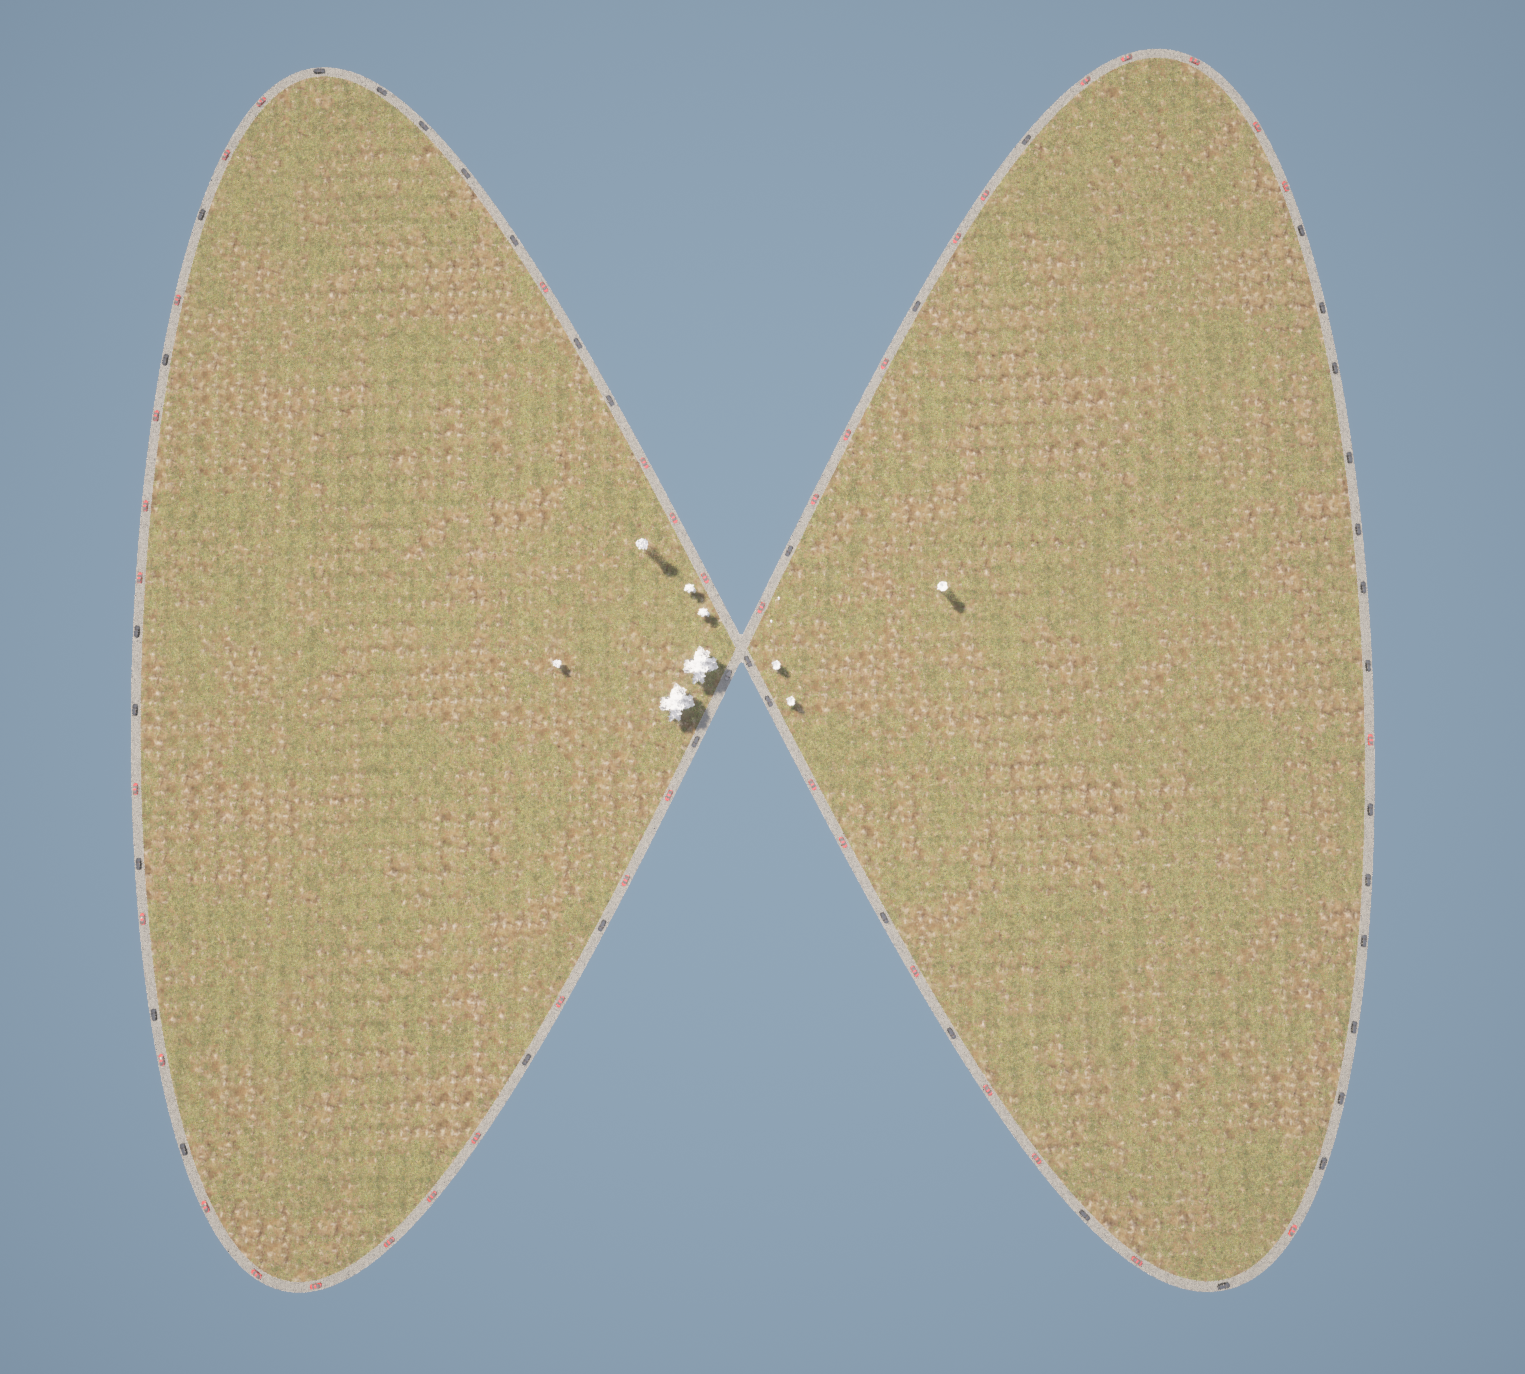
\includegraphics[width=\linewidth]{Screenshot from 2026-06-17 16-37-56.png}
        \caption{Overview of complete figure-eight}
        \label{fig:figure8_main}
    \end{subfigure}
    \hfill % Pushes the second subfigure to the right edge
    % Second Subfigure (Right)
    \begin{subfigure}[b]{0.48\linewidth}
        \centering
        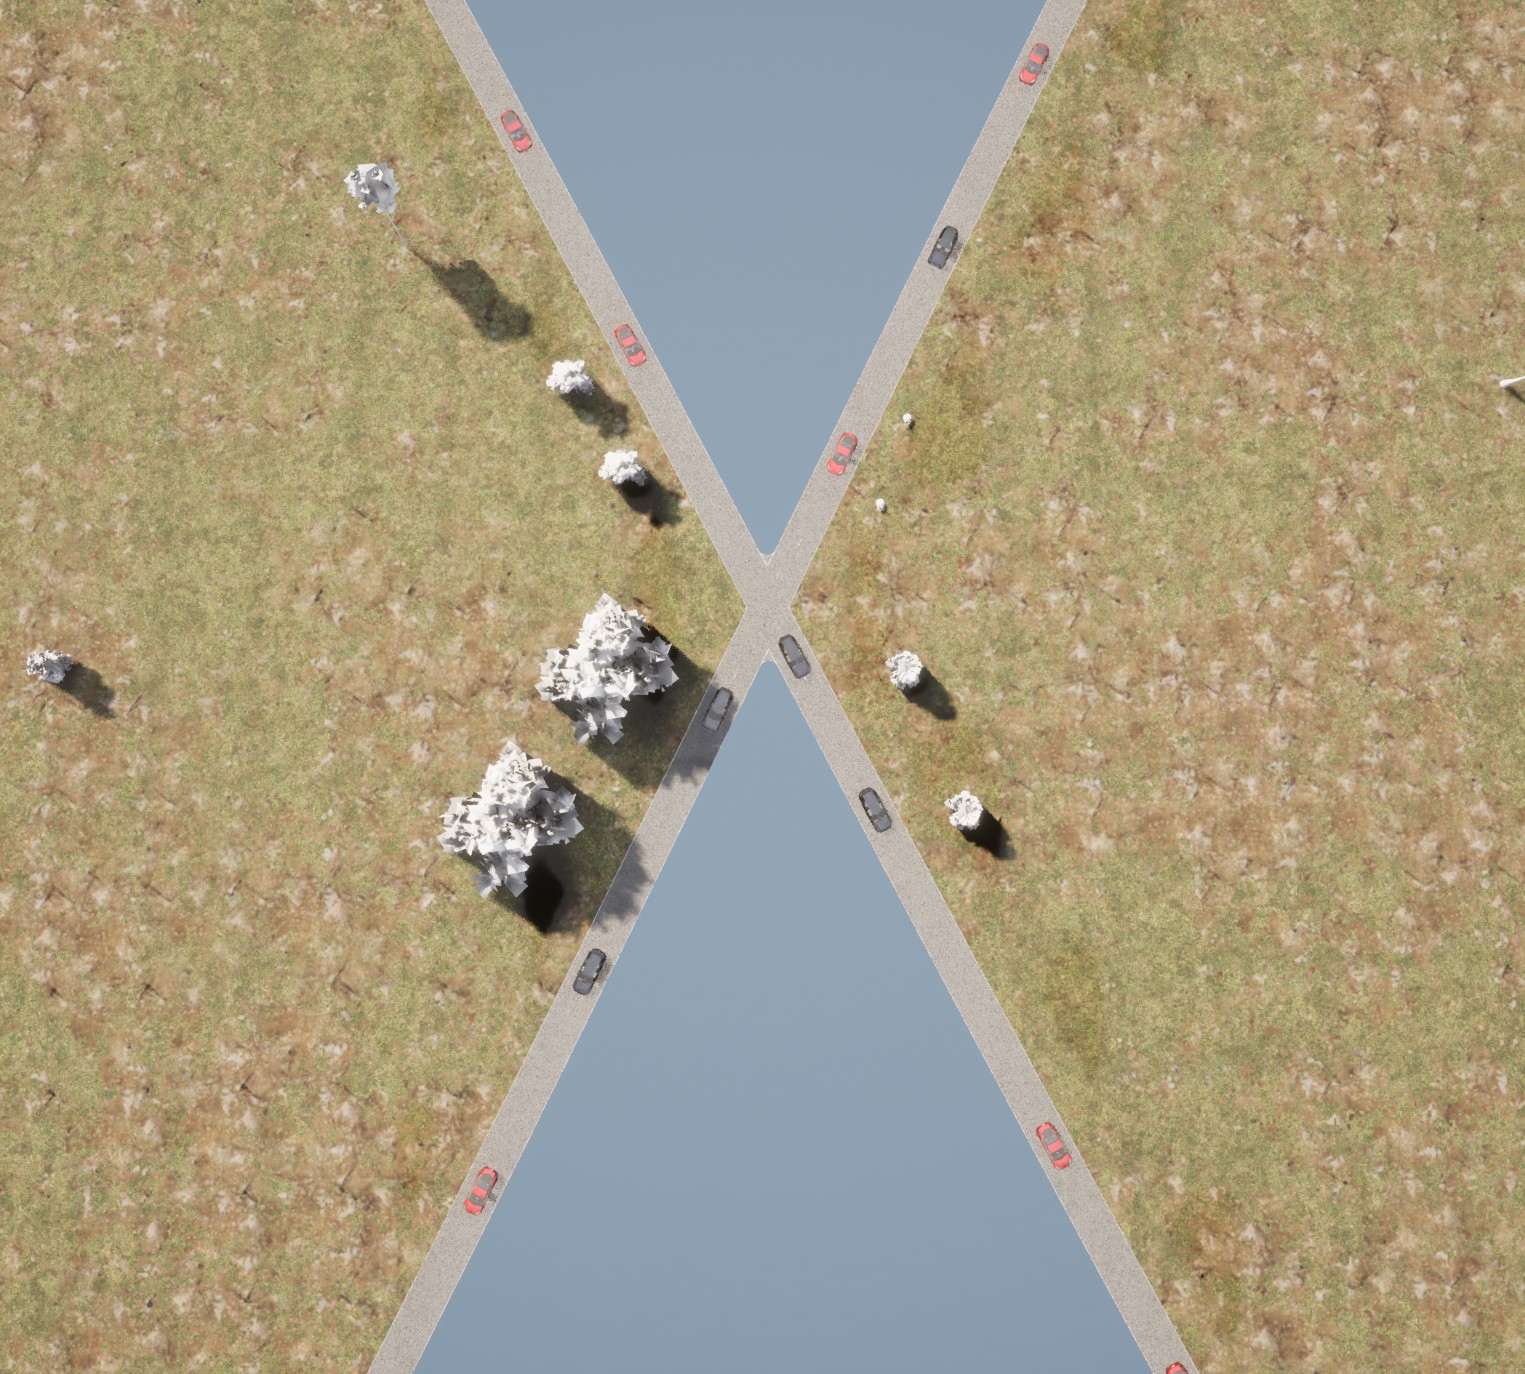
\includegraphics[width=\linewidth]{Screenshot from 2026-06-17 16-38-17.png}
        \caption{Figure-eight zoomed in at intersection}
        \label{fig:figure8_zoom}
    \end{subfigure}
    
    % Main Caption for the entire figure block
    \caption{Figure-eight Map: showing the complete map and a detailed close-up of the intersection with vehicles showing in red and black.}
    \label{fig:figure8_combined}
\end{figure}

On the figure-eight track, the position of an AV, is described by the parametric coordinate \(t\). However, the parametric coordinate is not suitable for the control strategies used in both simulations, since a difference between values of \(t\)  responds to the driven Euclidean distance. Nevertheless, the actual distance driven on the track is Geodesic. To resolve this issue, a distance mapper is used. At initialization, the distance mapper calculates the Arc Length \(L\)(m) using equation~\ref{arc length}
\begin{equation}
\label{arc length}
L =
\int_0^{2\pi}
\sqrt{
\left(\frac{dx}{dt}\right)^2 +
\left(\frac{dy}{dt}\right)^2
}
\,dt,
\end{equation} which is evaluated between 100000 equally spaced values of \(t\). The resolution of 100000 gives an accurate approximation of the true Geodesic distance by calculating the Euclidean distance of the small segments. The small segments are summed, and stored in a lookup table where each value of \(t\) corresponds to a geodesic distance \(s\)(m). Throughout the remainder of this chapter, linear interpolation is used to map from distance \(s\) to \(t\), section~\ref{Vehicle Fleet},  and from \(t\) to \(s\), section~\ref{Headway Control}.

\subsubsection{Vehicle Fleet and Initialization}
\label{Vehicle Fleet}
Two types of vehicles are used during the simulations, to reproduce a more realistic vehicle fleet. The vehicles used are the Tesla Model 3 RWD and the Audi e-tron 55, since these are listed in the standard CARLA vehicle library. Both vehicles differ in values with respect to weight \(m\)(kg), drag coefficient \(C_D\)(-), frontal area \(A_f(m^2)\), rolling resistance coefficient \(C_\text{rr}\)(-), gearbox ratio \(i_g\)(-), gearbox efficiency \(\eta_\text{gb}\)(-), wheel radius \(r_w\)(m), and motor efficiency \(\eta_\text{motor}\)(-). For the rolling resistance coefficient an average rolling resistance coefficient is used \parencite{swieczko2017tyre}. The gearbox efficiency value is assumed based on the typical efficiency of a planetary gearbox, which both vehicles use \parencite{lacock2023electric}. For motor efficiency, vehicle specific motor efficiency maps are used, which are extracted from current literature \parencite{rosenberger2024quantifying,thomas2021comparative} and shown in figure~\ref{fig:efficiency_contour}. The motor efficiency values are estimated using lookup tables, which are displayed in figure~\ref{fig:efficiency_lookups}. The remainder of the aforementioned values are displayed in table~\ref{vehicle specs}.

\begin{figure}[H] % 'htbp' is safer and more flexible than 'H'
    \centering
    % Subfigure A: Tesla Lookup
    \begin{subfigure}[b]{0.47\textwidth} % Slightly reduced width to safely fit margins
        \centering
        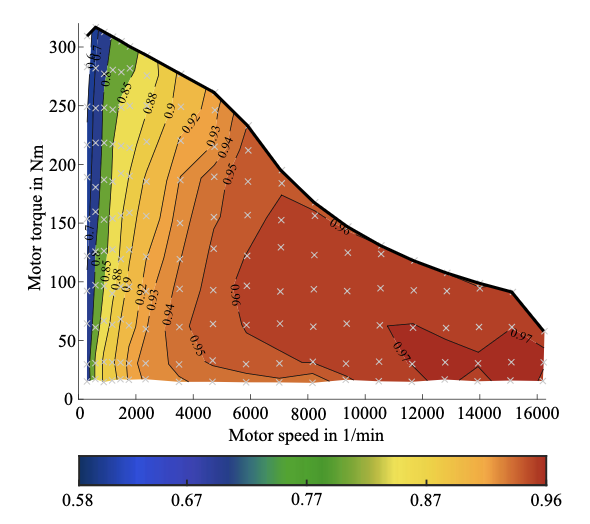
\includegraphics[width=\textwidth, height=4.5cm, keepaspectratio]{ContourTesla.png}
        \caption{Efficiency contour map of Tesla Model 3 RWD motor \parencite{rosenberger2024quantifying}.}
        \label{fig:tesla_lookup}
    \end{subfigure}% <-- This percent sign is CRITICAL. It prevents a hidden space.
    \hfill 
    % Subfigure B: Audi Lookup
    \begin{subfigure}[b]{0.47\textwidth}
        \centering
        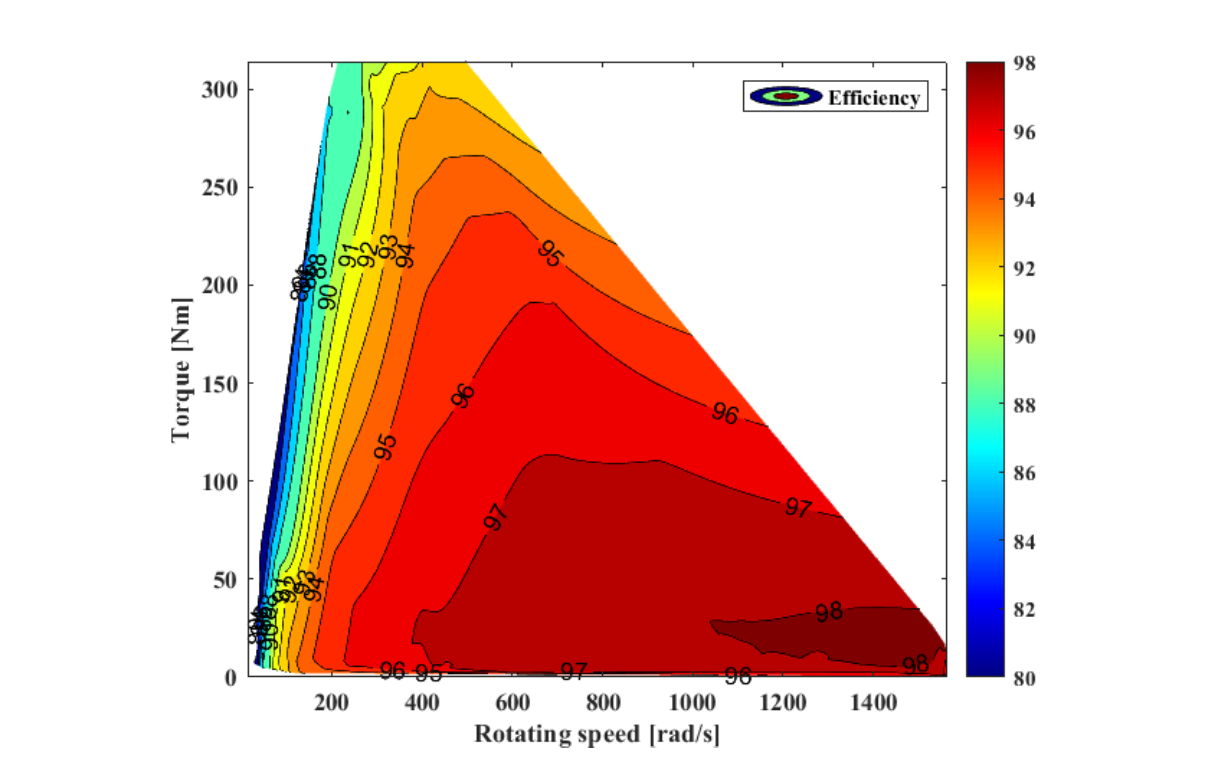
\includegraphics[width=\textwidth, height=4.5cm, keepaspectratio]{ContourAudi.png}
        \caption{Efficiency contour map of Audi e-tron 55 motor \parencite{thomas2021comparative}.}
        \label{fig:audi_lookup}
    \end{subfigure}
    
    \caption{Comparison of contour efficiency maps, Tesla Model 3 RWD vs. Audi e-tron 55.}
    \label{fig:efficiency_contour}
\end{figure}
\begin{figure}[H] % 'htbp' is safer and more flexible than 'H'
    \centering
    % Subfigure A: Tesla Lookup
    \begin{subfigure}[b]{0.47\textwidth} % Slightly reduced width to safely fit margins
        \centering
        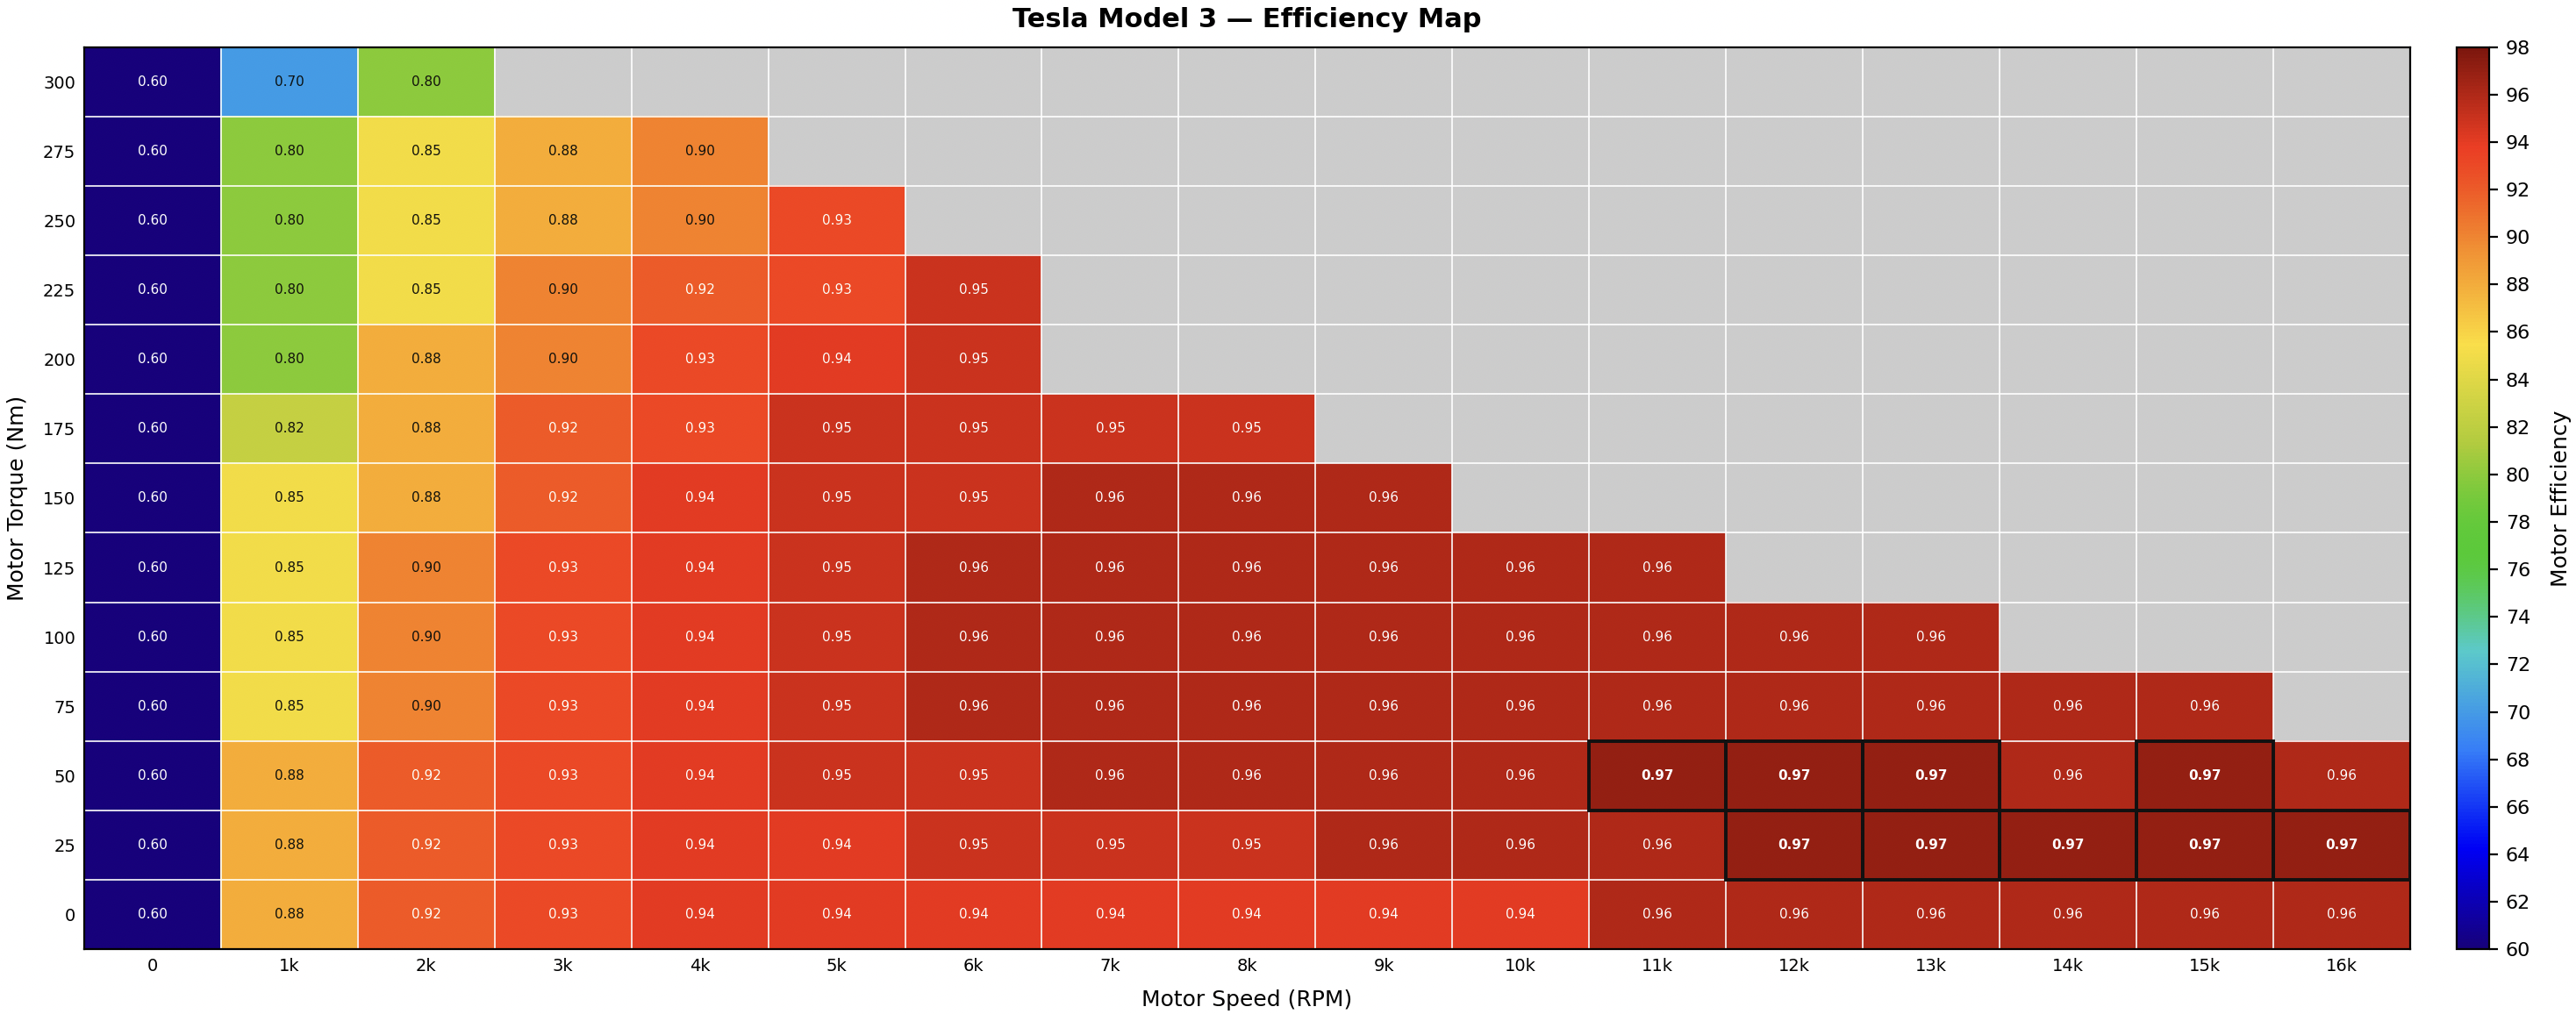
\includegraphics[width=\textwidth, height=4.5cm, keepaspectratio]{Table tesla.png}
        \caption{Lookup table of Tesla Model 3 RWD efficiency map}
        \label{fig:tesla_lookup}
    \end{subfigure}% <-- This percent sign is CRITICAL. It prevents a hidden space.
    \hfill 
    % Subfigure B: Audi Lookup
    \begin{subfigure}[b]{0.47\textwidth}
        \centering
        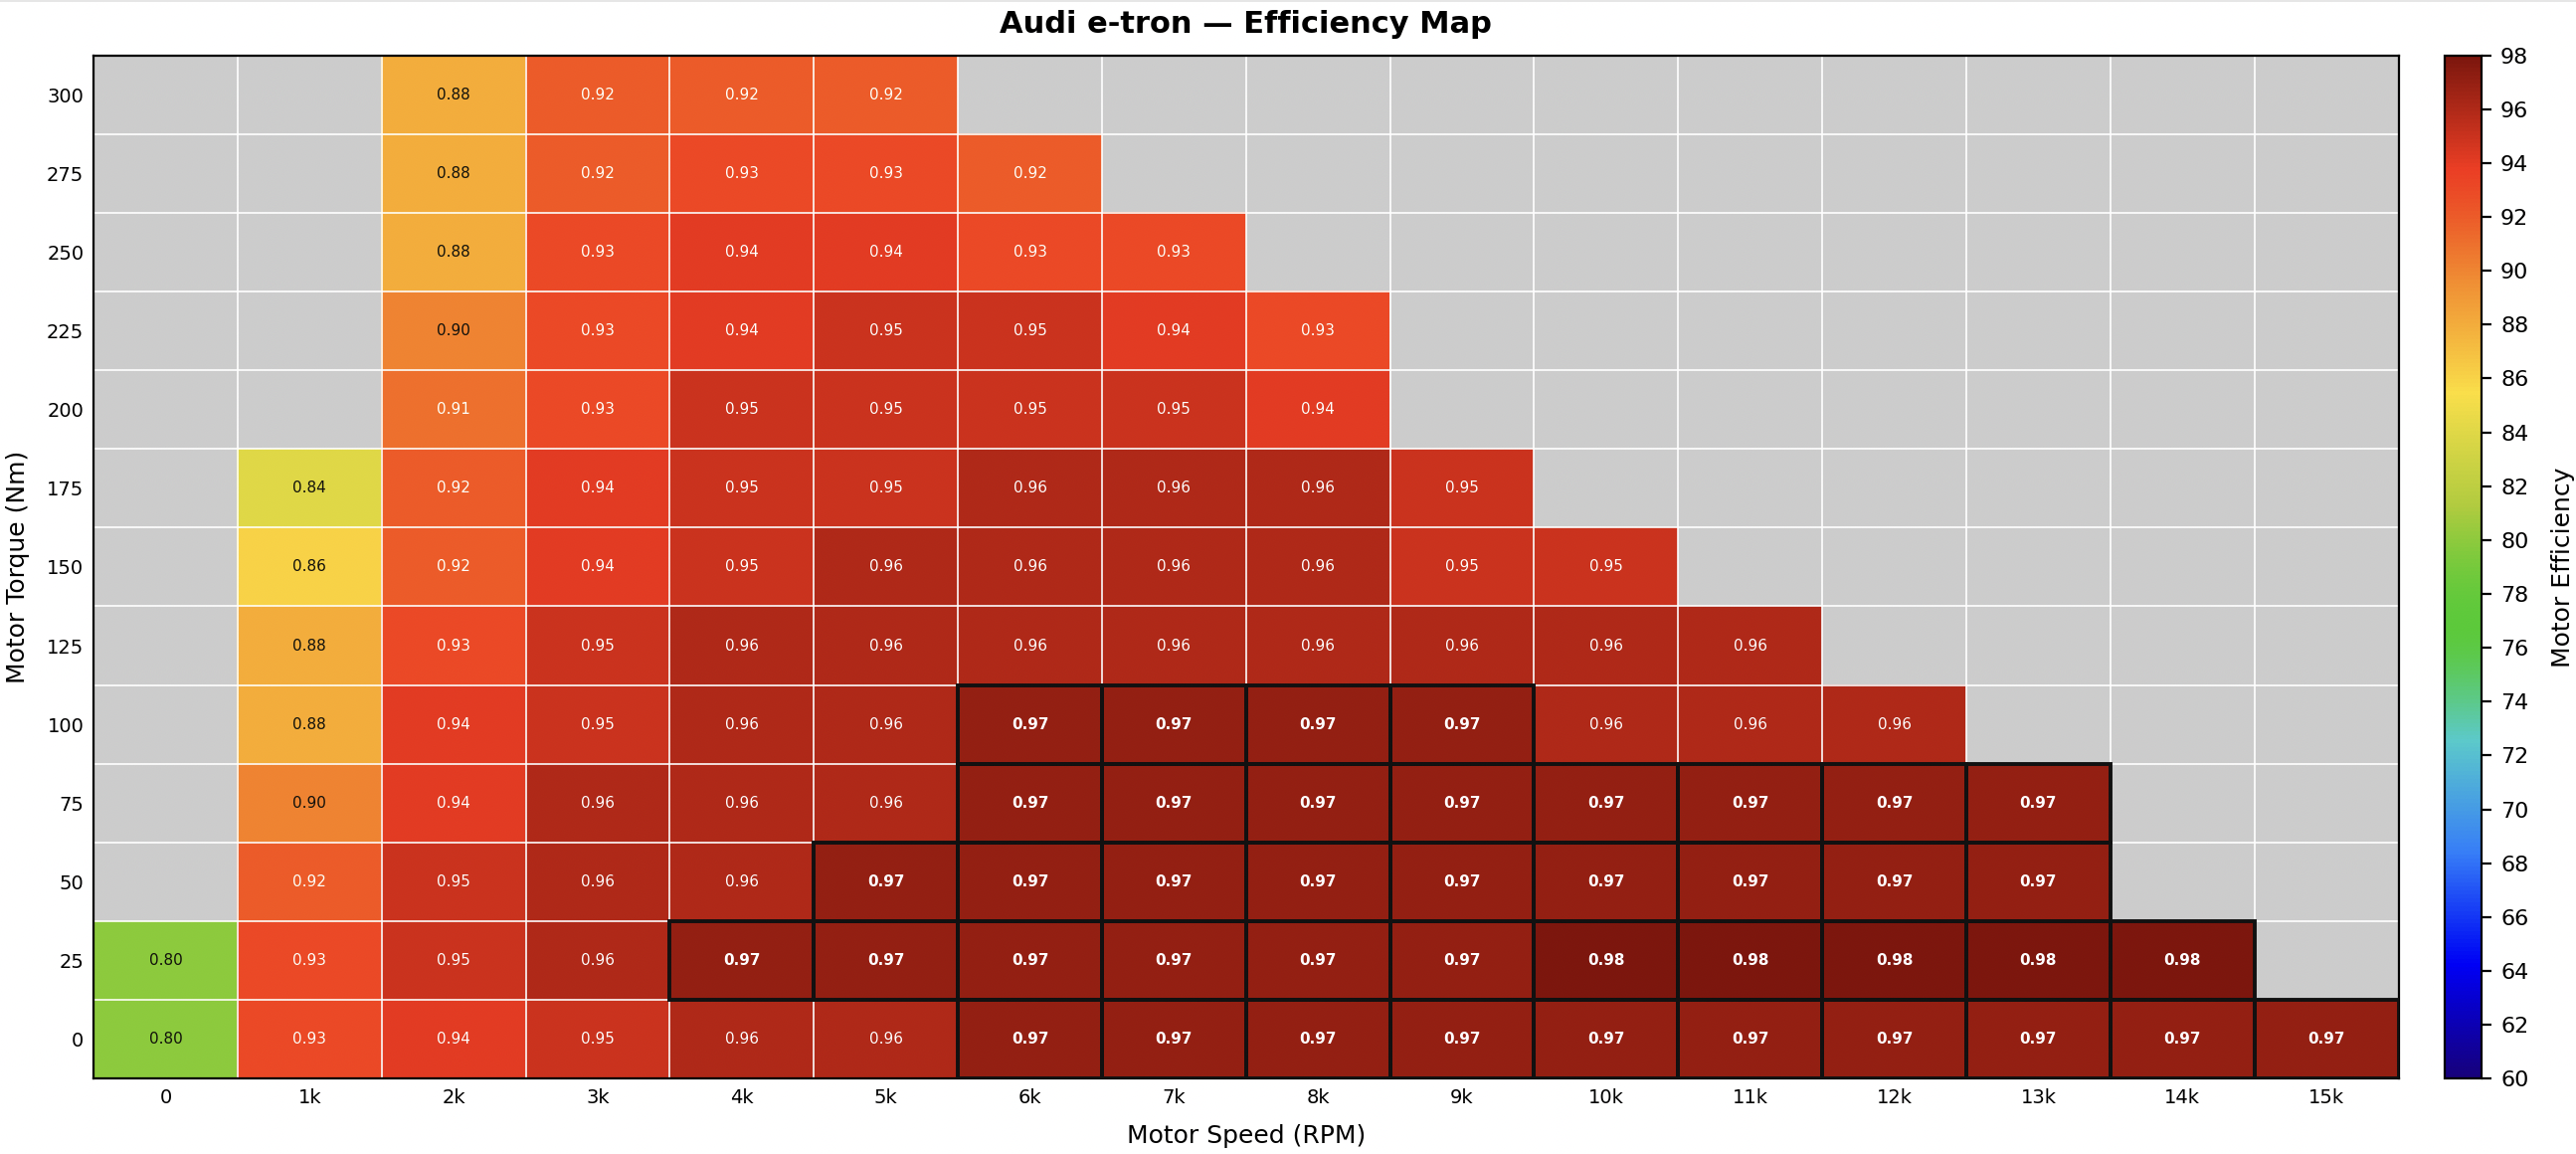
\includegraphics[width=\textwidth, height=4.5cm, keepaspectratio]{Table Audi.png}
        \caption{Lookup table of Audi e-tron 55 efficiency map}
        \label{fig:audi_lookup}
    \end{subfigure}
    
    \caption{Comparison of lookup tables generated from efficiency contour maps, Tesla Model 3 RWD vs. Audi e-tron 55.}
    \label{fig:efficiency_lookups}
\end{figure}

\begin{table}[H]
\centering
\caption{Per vehicle type specific parameters used during simulation: $^a$ sourced from manufacturer or press releases, $^b$ based on literature \parencite{swieczko2017tyre,rosenberger2024quantifying}, $^c$ assumed based on literature \parencite{lacock2023electric}.}
\begin{tabular}{lcc}

\toprule
\textbf{Parameter} & \textbf{Tesla Model 3 RWD} & \textbf{Audi e-tron 55} \\
\midrule
Weight, $m$ (kg) & 1931.0$^b$ & 2490.0$^a$ \\
Drag Coefficient, $C_D$ ($-$) & 0.23$^a$ & 0.28$^a$ \\
Frontal Area, $A_f$ ($\text{m}^2$) & 2.2$^a$ & 2.65$^a$ \\
Rolling Resistance Coeff., $C_{rr}$ ($-$) & 0.010$^b$ & 0.010$^b$ \\
Gearbox Ratio, $i_g$ ($-$) & 9.04:1$^b$ & 9.205:1$^a$ \\
Gearbox Efficiency, $\eta_{\text{gb}}$ ($-$) & 0.97$^c$ & 0.97$^c$ \\
Wheel Radius, $r_w$ (m) & 0.3468$^b$ & 0.3815$^a$ \\
\bottomrule
\end{tabular}
\label{vehicle specs}
\end{table}
With the vehicle types established, the vehicle initialization is started. Vehicle initialization consists of randomly spawning \(\frac{N}{2}+1\) Tesla Model 3s, and \(\frac{N}{2}\) Audi e-trons, with \(N\) the vehicle count, which is always an odd number. The placing of the vehicles starts each simulation run by placing the complete vehicle fleet \(N\) along the figure-eight track. The placement is performed using predefined target gaps \(d_\text{target}\) (m),  which is based on \(N\) and \(L\), and follows equation~\ref{Target} 
\begin{equation}
\label{Target}
    d_\text{target} = \frac{L}{N}.
\end{equation} The value of \(d_\text{target}\) is the input for the spawn positions of each vehicle along the track \(s_\text{target}\) (m), which follows equation~\ref{spawning}
\begin{equation}
\label{spawning}
    s_\text{target} = (j \times d_\text{target} + \epsilon\times d_\text{target}),
\end{equation}
with the vehicle number \(j\in\{1,N\}\), and the random spawn noise \(\epsilon\)(-). The computed spawn locations are linearly interpolated from \(s\) to \(t\), using the lookup table from section~\ref{Figure-eight track}, to align with the spawn approach used by CARLA. The value of \(t\) is compared to a list of safe spawn locations, which include all positions along the track except for the intersection. The intersection is excluded since two vehicles could spawn at the intersection at the same time, resulting in a direct crash during initialization. The vehicle, is therefore spawned at the safe spawn location which is closest to the value of \(t\) outside the intersection.

\subsubsection{Vehicle Controllers}
\label{Headway Control}
For driving along the track vehicles use a Headway Controller, which aims to maintain the target gap spacing between vehicles. The Headway controller adjusts based on the gap error \(e_\text{gap}(t)\)(m), between the target gap \(d_\text{t}\)(m), and the actual gap \(d_\text{actual}\)(m). \(d_\text{actual}\) corresponds to the Geodesic gap between the vehicle and its predecessor, which is derived using the lookup table generated by the Distance Mapper described in section~\ref{Figure-eight track}. This error is smoothed using an exponential moving average (EMA) filter, to account for a standard error between the math curve and the CARLA vehicle positions. 
\\\\
To adjust to errors in headway spacing, vehicles use a Proportional-Derivative (PD) controller, which takes \(e_\text{gap}(t)\) as input and computes a speed correction, \(u_\text{headway}\)(km/h), which follows equation~\ref{headwayeq}
\begin{equation}
\label{headwayeq}
    u_\text{headway}(t) = K_pe_\text{gap}(t)+ K_d\, \frac{d e_\text{gap}(t)}{dt},
\end{equation}
with the proportional gain \(K_p\ (km/h\cdot m)\) and the derivative gain \(K_d \ (km\cdot s/ m\cdot h)\). The speed correction is limited to ± 10 km/h, to ensure safe and comfortable control actions for vehicles in both simulations. Especially in the FAS simulation this limit is necessary, since the headway gap between a vehicle waiting on a red light, and its predecessor which just passed the red light, can grow very large. The large gap can result in a large headway error, which leads to a high speed correction demanded by the PD-controller, The high speed correction leads to maximum throttle when the light switches to green. Since this behavior is not aligned with realistic vehicle behavior at traffic lights, the limit of ±10 km/h is applied. 
\\\\
To respond to the various speed demands from the headway controller, barrier controller or vehicle response to the FAS controller, each vehicle uses a longitudinal controller. This controller, implemented as a Proportional-Integral-Derivative (PID) controller, translates the error between current speed and target speed,  \(e_\text{speed}(t)\), in various throttle and brake commands \(u_\text{throttle,brake}\), which follows equation~\ref{long}
\begin{equation}
\label{long}
    u_\text{throttle,brake} =  K_pe_\text{speed}(t)+ Ki \int_0^te_\text{speed}(\tau)d\tau + K_d\, \dot{e}_\text{speed}(t), 
\end{equation}
The \(u_\text{throttle,brake}\) commands are limited to ±1, where a command of +1.0 represents maximum throttle, and -1.0 represent maximum braking.  
\\\\
 Lastly, lateral control of the vehicles is handled by computing a look-ahead point on the track, which is done by advancing the current trajectory parameter \(t\) with a look-ahead step, which scales with the track radius, R. The steering is performed based on the signed angle between the vehicles current heading and the direction toward the look-ahead point. The output is bounded to ±1, which aligns with CARLAs steering input range.
\subsubsection{Energy Consumption Model}
\label{energy model explain}
The energy consumption model tracks the actual power drawn or restored from the battery during each simulation step, accounting for drivetrain losses in both directions. The battery power differs from the mechanical power delivered at the wheels during propulsion and regeneration. During propulsion efficiency losses in both motor and gearbox require more delivered battery power than the mechanical power at the wheels, whereas during regenerative braking not all recovered energy is completely restored into battery power, due to similar efficiency losses in the opposite direction. The calculation below therefore details how power consumed or restored at the wheels converts to actual battery power in three steps.  
\\\\
First, the total longitudinal force \(F_\text{total}\)(N)~\ref{Ftotal} acting on the wheels during driving is calculated, which consists of acceleration force \(F_\text{inertia}\)(N), aerodynamic drag force \(F_\text{aero}\)(N), and rolling resistance force \(F_\text{rolling}\)(N) \begin{equation}
\label{Ftotal}
    F_\text{total} = \underbrace{ma}_{F_\text{inertia}} + \underbrace{\tfrac{1}{2}\rho C_d A v^2}_{F_\text{aero}} + \underbrace{C_\text{rr}mg}_{F_\text{rolling}},
\end{equation} with acceleration \(a (m/s^2)\), air density \(\rho (kg/m^3)\), vehicle speed \(v\)(m/s), and gravitational acceleration \(g (m/s^2)\). The vehicle speed is directly extracted from the value reported by CARLA. However, CARLA does not report vehicle acceleration, therefore acceleration is computed from the finite difference of vehicle speed between each timestep. Since the calculation is found to be sensitive to simulation noise, the computed acceleration is smoothed using an EMA filter, using \(\alpha_\text{acceleration}\) listed in table~\ref{tab:simulation_parameters}. All other necessary values are extracted from table~\ref{vehicle specs}, and the values are selected based on the defined vehicle type, Tesla or Audi.
\\\\
Second, following equation~\ref{mech}, which multiplies total longitudinal force with velocity, the instantaneous mechanical power demand at the wheels is derived, which describes the power that must be delivered at the wheels at the specific moment 
\begin{equation}
\label{mech}
    P_\text{mech}= F_\text{total}\cdot v.
\end{equation}
In principle, the computed \(P_\text{mech}\) differs from the actual battery power demand \(P_\text{bat}\)(W), due to losses in the transmission and the electric motor during propulsion, and similar losses during regenerative braking \parencite{luin2019microsimulation}. To account for gearbox losses, a constant gearbox efficiency factor is used \(\eta_\text{gb}\) and for motor losses the vehicle specific motor efficiency \(\eta_\text{motor}\) is used. This motor efficiency is not a fixed value, as efficiency depends on motor shaft speed \(N_\text{motor}\)(RPM) and motor torque \(\tau_\text{motor}\)(Nm), which are derived from vehicle speed and \(F_\text{total}\). The motor shaft speed follows equation~\ref{shaft speed}
\begin{equation}
\label{shaft speed}
    N_\text{motor} = \frac{i_g\cdot v \cdot 60}{2 \cdot\pi\cdot r_w},
\end{equation}
and motor torque is dependent on propulsion or regenerative braking and follows equation~\ref{torque}
\\
\begin{equation}
\label{torque}
\tau_{\text{motor}} = \begin{cases} 
\displaystyle\frac{F_{\text{total} \, r_w}}{i_g \ \,\eta_\text{gb}} & \text{if } F_{\text{total}} \geq 0 \quad \text{(propulsion)} \\[2ex] 
\displaystyle\frac{F_{\text{total} \, r_w \, \eta_\text{gb}}}{i_g} & \text{if } F_{\text{total}} < 0 \quad \text{(regenerative braking)},
\end{cases}
\end{equation}
whereas during propulsion more motor torque is needed to overcome losses, and during regenerative braking, a smaller amount of torque is produced by the braking \parencite{luin2019microsimulation}.
\\\\
Third, the determined values, \(N_\text{motor}\) and \(\tau_\text{motor}\), are used to extract vehicle specific motor efficiency \(\eta_\text{motor}\), from a lookup table, from which a figure is shown in figure~\ref{fig:efficiency_lookups}. The efficiency value is estimated, by bilinear interpolation between the adjacent cells in the lookup table.  
The actual battery power demand is calculated using equation~\ref{Pbat}, which utilizes the derived \(\eta_\text{motor}\), \(\eta_\text{gb}\), and \(P_\text{mech}\) \parencite{chen2021review}, where the sign of \(P_\text{mech}\) illustrates propulsion or regenerative braking \begin{equation}
\label{Pbat}
P_{\text{bat}} = \begin{cases}
\displaystyle\frac{P_{\text{mech}}}{\eta_\text{gb}\,\eta_\text{motor}} & \text{if } P_{\text{mech}} \geq 0 \quad \text{(propulsion)} \\[2ex]
P_{\text{mech}} \cdot \eta_\text{gb}\,\eta_\text{motor} & \text{if } P_{\text{mech}} < 0 \quad \text{(regenerative braking)}
\end{cases}.
\end{equation}
During propulsion, \(P_\text{mech}\) is divided by \(\eta_\text{gb}\) and \(\eta_\text{motor}\), to reflect the additional power drawn from the battery to overcome the losses. On the other hand, during braking, the power is multiplied with \(\eta_\text{gb}\) and \(\eta_\text{motor}\), which reflects the fraction of power actually regenerated to the battery due to regenerative braking \parencite{luin2019microsimulation}.
\\\\
This energy consumption model uses a few simplifying assumptions. First, since the figure-eight is flat, no gradient force is considered. Second, the motor efficiency maps are estimates from other researchers, due to limited availability of vehicle specific maps. Third, the Audi e-tron efficiency map excludes inverter efficiency, whereas the Tesla Model 3 map includes the inverter efficiency. Since no inverter efficiency coefficient could be found for the Audi e-tron, the inverter inefficiency is neglected, and therefore the efficiency of the Audi e-tron is being overestimated. Fourth, efficiency maps had empty regions, which are assumed to have low efficiency of 0.60. Fifth, the motor is assumed to be equally efficient during propulsion and regenerative braking. Finally, auxiliary loads, like heating, ventilation, and air conditioning are neglected, since it is a constant across both simulations. However, since all the assumptions influence both simulations identically, they do not affect the relative comparison.

\subsection{Experimental Design and Parameters}
\label{Experimental Design}
The barrier and FAS controller  are evaluated under identical conditions using the simulation framework~\ref{Sim environment}. This section describes how stochastic initial conditions were used across both controllers to evaluate robustness of the results.
\subsubsection{Traffic Density and Vehicle Initialization}
\label{Experimental setup}
To analyze the performance of both intersection control strategies under varying traffic density, four vehicle counts are evaluated: \(N \in\{51,61, 71, 81\}.\) To account for variability in initial conditions, each vehicle count is simulated over 30 independent simulation runs with spawn noise \(\epsilon\) of up to ±20 \%. The spawning follows formula~\ref{spawning} and an example of spawning with noise is displayed in figure~\ref{fig:figure8_zoom}. To ensure that any observed difference in KPIs can solely be attributed to the intersection management strategy, each simulation run uses a reproducible random seed which ensures that run \(k\) of the barrier controller uses identical conditions as run \( k\) of the FAS controller. 
\subsubsection{Simulation Phases and Parameters}
Simulations are performed using synchronous mode at a fixed timestep of \(\Delta t\)(s). This combination allows for precision between simulations and limits computational costs. With \(\Delta t\) in place, the simulation starts with a warm-up phase, during this phase vehicles are held stationary with the handbrake active, this is done to ensure that CARLA can spawn the vehicles correctly.  Next, a ramp-up phase starts, during this phase vehicles ramp-up to the target speed. During this phase the headway correction \(u_\text{headway}\), discussed in section~\ref{Headway Control}, is inactive, but both intersection management strategies are active to prevent collisions at the intersection during ramp-up. After the ramp-up phase, the evaluation-phase begins in which the headway controller also takes action. The durations of each phase and the simulation conditions are summarized in table~\ref{tab:sim_params}.
\\\\


\begin{table}[H]
\caption{Parameters used during all simulations }
\centering
\begin{tabular}{ll}
\toprule
\textbf{Parameter} & \textbf{Value} \\
\midrule
Simulation Time & 1800 s \\
Track Length (\(L\)) & 2347.4 m \\
Timestep (\(\Delta t\)) & 0.05 s \\
Warm-up Phase & 5 s \\
Ramp-up Phase & 12.5 s \\
Target Speed (\(v^*\)) & 30 km/h \\
Vehicle Counts ($N$) & 51, 61, 71, 81 \\
Spawn Noise (\(\epsilon\)) & $\pm$0.20\\
Runs per $N$ & 30 \\

\bottomrule
\end{tabular}

\label{tab:sim_params}
\end{table}




\subsection{Performance Measurement and Validation}
\label{Key Performance Indicators}
During the simulations, four KPIs are recorded. These KPIs form the basis for the quantitative analysis. The remainder of this section explains the key performance indicators and the validation approach.

\subsubsection{Throughput, Delay, Energy, and Safety Violations}
Throughput is measured as the number of vehicles that cross the intersection per unit of time \parencite{soltani2025communication}. In the simulation environment, vehicles can cross the conflict point from two sides, either halfway at \(t=\pi\) or at the wraparound point \(t = 0 \) (equivalently \(t=2\pi\)). A crossing is counted if a vehicle passes the conflict point. The total throughput rate \(I\)(veh/s), is the total number of crossings \(N_c\)(veh), divided by the elapsed time \(T\), which follows equation~\ref{throughput}
\begin{equation}
\label{throughput}
I = \frac{N_\text{c}}{T}.   
\end{equation}  
\\\\
Delay time is commonly measured in traffic studies to evaluate efficiency of intersection management systems \parencite{soltani2025communication}. It demonstrates the extra time it takes to traverse the intersection compared to a free flow situation. To compute delay time, the lap times of vehicles are calculated. To ensure that no delay occurs from the warm-up and ramp-up phase, the counting starts after completion of the two phases. After completion, the position of each vehicle is captured and stored. If the corresponding vehicle crosses its stored position again, it has completed a lap and the lap time is recorded. 
For calculating the per vehicle delay time \(t_\text{delay}\)(s), a free flow lap time is calculated. This lap time is found by simulating a complete lap, with only one vehicle, moving at the target speed. From the free flow lap time  \(t_\text{delay}\) can be calculated, which follows equation~\ref{Delay}
\begin{equation}
\label{Delay}
    t_\text{delay} = t_\text{actual}-t_\text{ideal},
\end{equation}
with the actual lap time \(t_\text{actual}\)(s), and the free flow lap time \(t_\text{ideal}\)(s). To find the per simulation delay, all values of \(t_\text{delay}\) are accumulated into total delay.
\\\\
Energy consumption is measured as the total battery power of all vehicles during a simulation run. For calculation, the per vehicle energy model described in section~\ref{energy model explain} is used. The per vehicle battery power is accumulated over time \parencite{chen2021review}, which follows~\ref{energy} \begin{equation}
\label{energy}
    E_\text{total} = \frac{1}{3.6\times10^6}\int_0^T P_\text{bat}dt, 
\end{equation} where \(\frac{1}{3.6\times10^6}\) is used to convert from J to kWh.
\\\\
The amount of safety violations is evaluated as the number of near-crash collisions at the intersection. A near-crash collision occurs if two simultaneously approaching vehicles from opposing sides cross within a predefined safety distance of each other. If the actual gap at the intersection falls below the predefined threshold value, a near-crash collision is counted.  The number of safety violations \(N_v\)(violations), is accumulated during simulation and divided by the elapsed time T(s) to get the safety violation rate S (violations/s), which follows equation~\ref{Safetyviolationseq}
\begin{equation}
\label{Safetyviolationseq}
       S = \frac{ N_v}{T}.
\end{equation}




\subsubsection{Validation Approach}
\label{System Validation}
To ensure the simulation framework produces reliable and realistic results, two validation steps are performed after the experiments.
\\\\
First, the headway controller is validated by verifying convergence to the target spacing during the evaluation phase for the barrier controller. Convergence is considered successful when all vehicles maintain a gap within 2.5 m from the target spacing. This validation is performed by manually comparing the target headway spacing to the actual headway spacing. In addition, a plot of both of the aforementioned parameters is created and manually inspected after each run.    
\\\\
Second, the four KPIs are validated. Throughput is validated by manual inspection and comparison to the theoretical maximum. The theoretical maximum is calculated based on the number of vehicles, the length of the track, and the target speed. The simulated throughput value is verified to remain within this theoretical maximum across all runs. A similar approach is used to validate delay time. The approach consists of a comparison of the actual lap time to the theoretical minimum, which is calculated from the length of the track and the target speed. Validation of the energy consumption model is done by comparing output of the simulations with publicly available energy consumption figures. The validation is performed to confirm that the power demand model produces realistic values. Lastly, the safety violations are validated by manual inspecting the violation measurement during simulations. 
\\\\









\newpage


\section{Results}
\label{Results}
This section describes results for both barrier and FAS controller. Starting with the results of the validation approach, followed by the vehicle behavior (i.e. speed, target gap, acceleration and energy consumption), followed by the barrier controller performance, and lastly the KPI comparison.

\subsection{Simulation Output Validation}
Simulations showed that the headway gaps converged within the 2.5 m threshold across all simulations, which figure~\ref{fig:gapmean} supports by showing the target headway gap and the mean across all simulations per \(N\). The figure highlights that the mean headway gap sits tightly around the target gap for each \(N\).\\\\
Figure~\ref{fig:theoretical max} shows that throughput remained within the theoretical maximum across all simulations. Similarly, recorded lap times showed that the lap times remained above the theoretical minimum lap when the average speed was similar to the target speed. For some vehicles the lap time was found to be lower than the minimal lap time, due to a higher average speed. 
\\\\
The energy model is validated against the Tesla Model 3 RWD WLTP consumption of 0.136 kWh/km \parencite{rosenberger2024quantifying}, as this is the only vehicle for which a citable source is available. Table~\ref{tab:vehicle_energy_filtered} shows that the mean Tesla Model 3 RWD energy consumption range from 0.072 to 0.156 kWh/km. The 0.072 kWh/km corresponds to the barrier controller, which is 47\% below the WLTP figure, whereas using the FAS controller the energy usage is 14.7\% above the WLTP figure. These opposing directions align with the hypothesis that frequent stop-and-go behavior leads to higher energy consumption, whereas cruising at constant speed with small fluctuations in acceleration results in lower energy consumption. In addition, table~\ref{tab:vehicle_energy_filtered} shows that the Audi e-tron consumes more energy per km, which aligns with the higher \(F_\text{total}\), due to the differences in vehicle specific parameters, table~\ref{vehicle specs}.  All in all, the energy model produces realistic values despite the models simplifying assumptions.
\\\\
The counted safety violations were directly compared to videos of the simulations. The videos showed only safety violations at near simultaneous arrival, which is is line with the setup of the performance indicator.  

\begin{figure}[H]
    \centering
        % Set height instead of width to make them level
        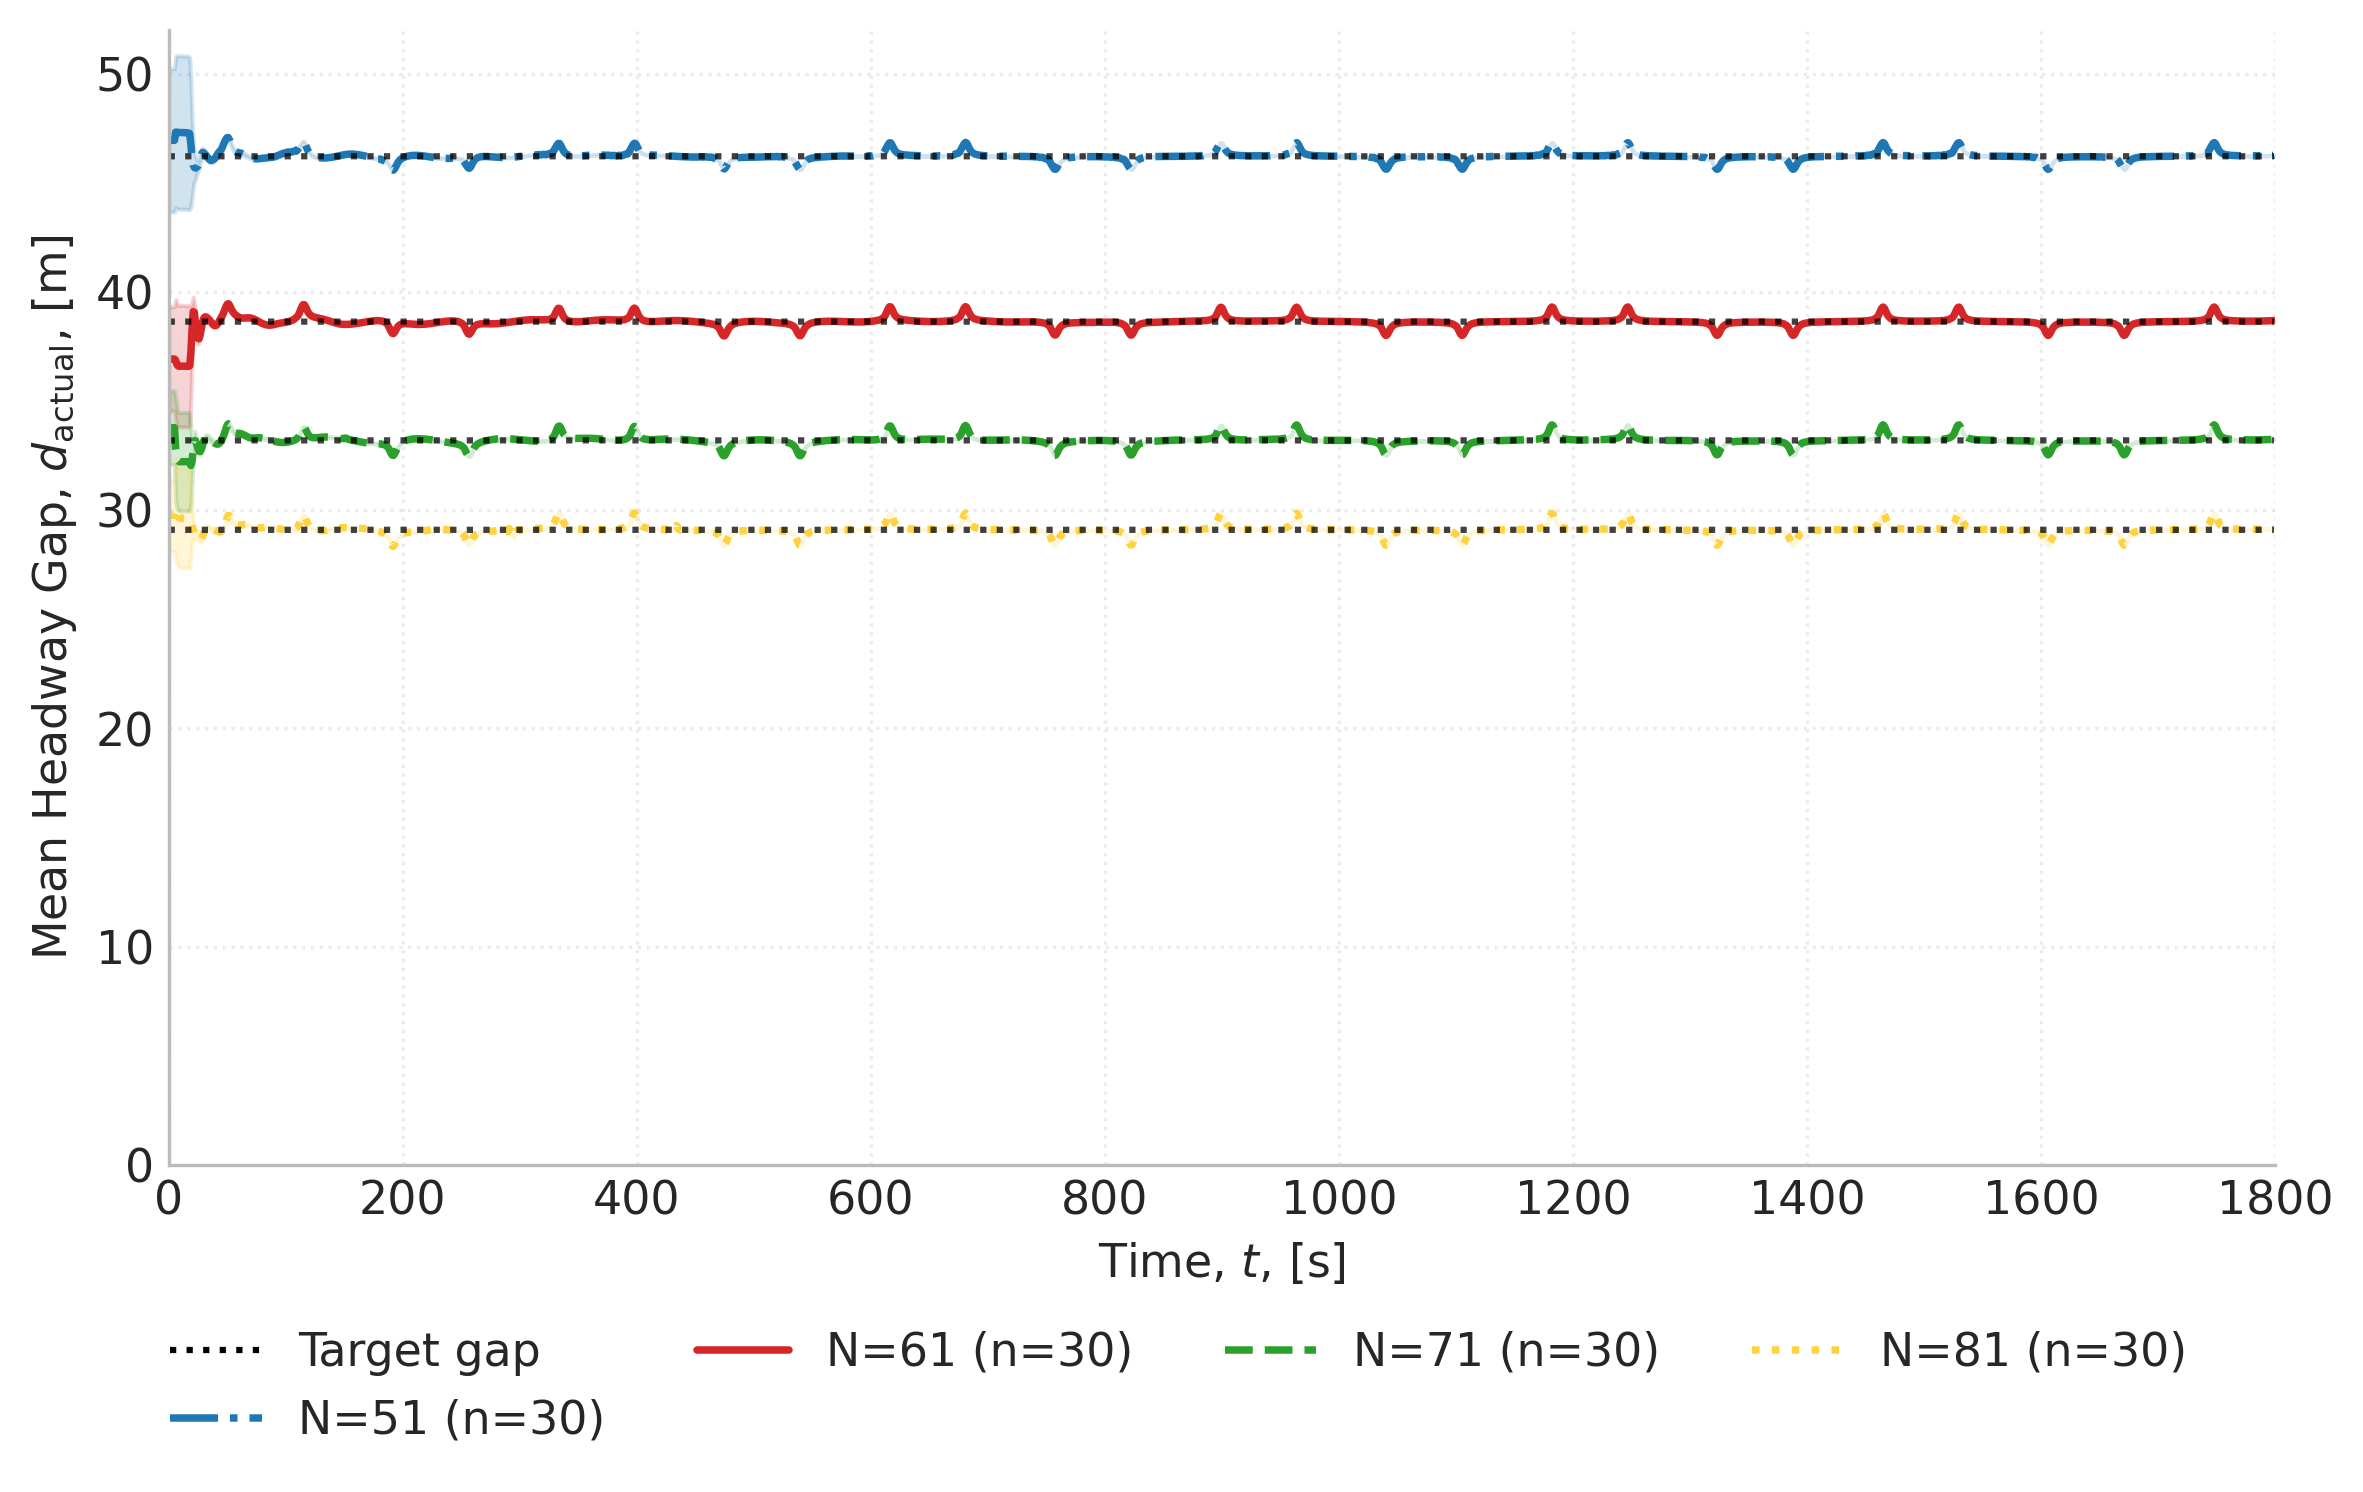
\includegraphics[ width=\linewidth, keepaspectratio]{MeanGap.png}
        \caption{Mean headway gap ± 95\% CI and target gap per vehicle density \(N = \{51,61,71,81\}\) over simulation time}
        \label{fig:gapmean}
        \end{figure}
    
    \begin{figure} [H]
        \centering
        % Set matching height here
        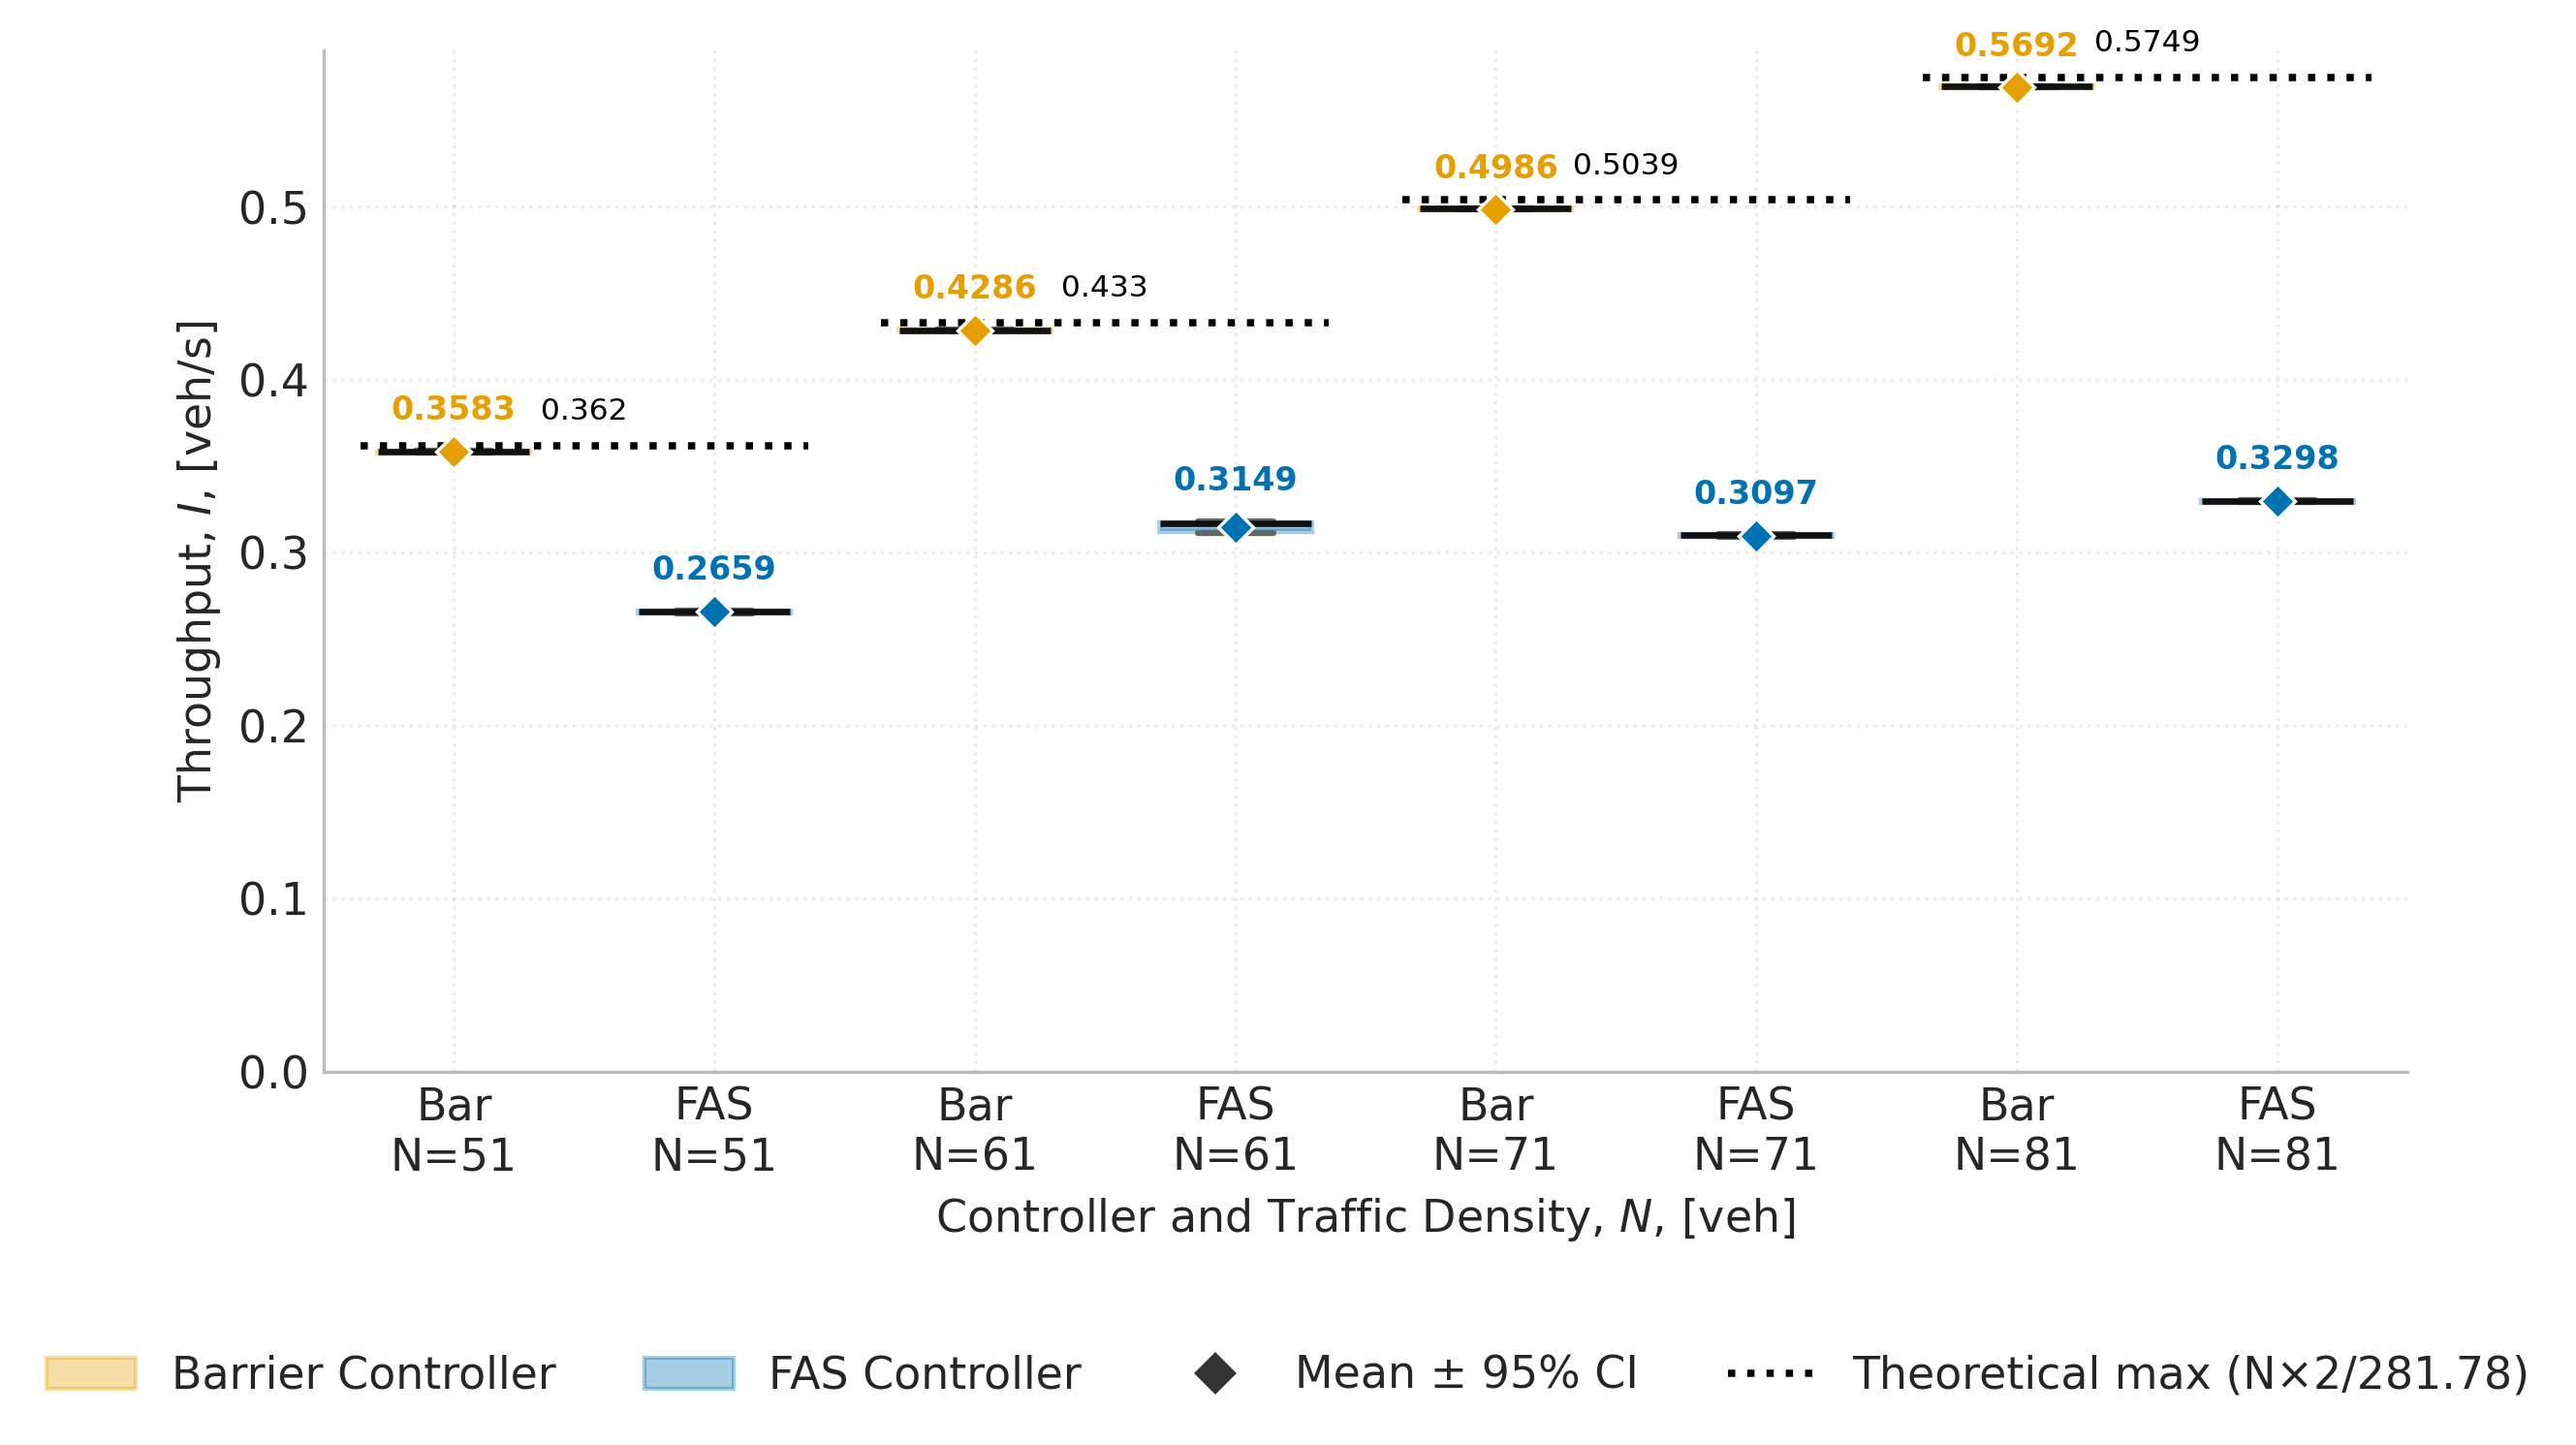
\includegraphics[ width=\linewidth, keepaspectratio]{throughput-per-demand.png}
        \caption{Boxplot with additional mean and 95\% CI per controller for each \(N\), and theoretical maximum for all \(N\)}
        \label{fig:theoretical max}
    \end{figure}

\begin{table}[H]
\centering
\caption{Vehicle Specific Energy Consumption in kWh/km, displaying mean $\pm$ 95\% CI, for all traffic densities across all controllers}
\label{tab:vehicle_energy_filtered}
\begin{tabular}{lllr}
\hline
\textbf{Controller} & \textbf{Traffic Density} & \textbf{Vehicle Type} & \textbf{Energy (kWh/km) $\pm$ 95\%CI} \\ \hline
FAS Controller     & 51 & Audi e-tron 55    & $0.139559 \pm 0.000609$ \\
FAS Controller     & 61 & Audi e-tron 55    & $0.144853 \pm 0.000474$ \\
FAS Controller     & 71 & Audi e-tron 55    & $0.181942 \pm 0.000235$ \\
FAS Controller     & 81 & Audi e-tron 55    & $0.195923 \pm 0.000393$ \\
FAS Controller     & 51 & Tesla Model 3 RWD & $0.112200 \pm 0.000489$ \\
FAS Controller     & 61 & Tesla Model 3 RWD & $0.115922 \pm 0.000438$ \\
FAS Controller     & 71 & Tesla Model 3 RWD & $0.141730 \pm 0.000158$ \\
FAS Controller     & 81 & Tesla Model 3 RWD & $0.155531 \pm 0.000238$ \\ \hline
Barrier Controller & 51 & Audi e-tron 55    & $0.089171 \pm 0.000266$ \\
Barrier Controller & 61 & Audi e-tron 55    & $0.089223 \pm 0.000309$ \\
Barrier Controller & 71 & Audi e-tron 55    & $0.089285 \pm 0.000326$ \\
Barrier Controller & 81 & Audi e-tron 55    & $0.090644 \pm 0.000288$ \\
Barrier Controller & 51 & Tesla Model 3 RWD & $0.071781 \pm 0.000196$ \\
Barrier Controller & 61 & Tesla Model 3 RWD & $0.072030 \pm 0.000387$ \\
Barrier Controller & 71 & Tesla Model 3 RWD & $0.071914 \pm 0.000294$ \\
Barrier Controller & 81 & Tesla Model 3 RWD & $0.072851 \pm 0.000220$ \\ \hline
\end{tabular}
\end{table}

\subsection{Single-Vehicle Behavior Profiles}
 This section analysis the behavior of a single vehicle of both controllers under identical conditions. 

\subsubsection{Barrier Controller Vehicle Behavior}
The vehicle behavior of the barrier controller is illustrated in figure~\ref{fig:barrier}, showing respectively acceleration, speed, following gap, and power for one vehicle from run 1, with \(N=61\). \\\\
The speed profile, figure~\ref{fig:speed61}, shows that after the initial ramp up phase, speed rapidly settles around the target speed of $8.33 \ m/s^2$. During the ramp up phase, the vehicle accelerates from the spawn position and briefly overshoots the target speed. After this overshoot, the speed PID-controller quickly corrects the actual speed to the target speed. During the remainder of the simulation actual speed remains closely around the target speed, with small recurring fluctuations. 
\\\\
The following gap, figure~\ref{fig:gap61}, confirms both steady-state behavior and the small recurring gap error. The first part of the figure shows the spawn noise, where-after the gap rapidly converges to the target gap of 36.6 (m), and remains there for the remainder, with small recurring fluctuations.  
\\\\
The acceleration profile, figure~\ref{fig:accel61}, shows a clear ramp up phase, during which acceleration fluctuates between, $+6$ and $-7$ \(m/s^2\). After the ramp up phase, it can be seen that acceleration settles around 0 \(m/s^2\), with small oscillations. The absence of large peaks in acceleration during the evaluation phase follow from the near steady state driving at both target speed and target gap.  
\\\\
Lastly, figure~\ref{fig:power61}, describes the drive power profile. During the ramp-up phase the vehicle accelerates from rest to the target speed, resulting in propulsion peaks. After this phase the acceleration stabilizes and speed remains around target; therefore, power settles to small propulsion during the remainder of the simulation time. The power profile is positive during the whole simulation, except for one moment during the ramp-up phase, which shows energy regeneration, due to the speed overshoot visible in figure~\ref{fig:speed61}, which leads to the deceleration peak visible in figure~\ref{fig:accel61}.
\\\\
Overall, the barrier controller simulation shows smooth vehicle behavior, with vehicles maintaining target speed and target gap, resulting in small fluctuations in both acceleration and drive power.   



\begin{figure}[H]
    \centering
    \begin{subfigure}[b]{0.48\textwidth}
        \centering
        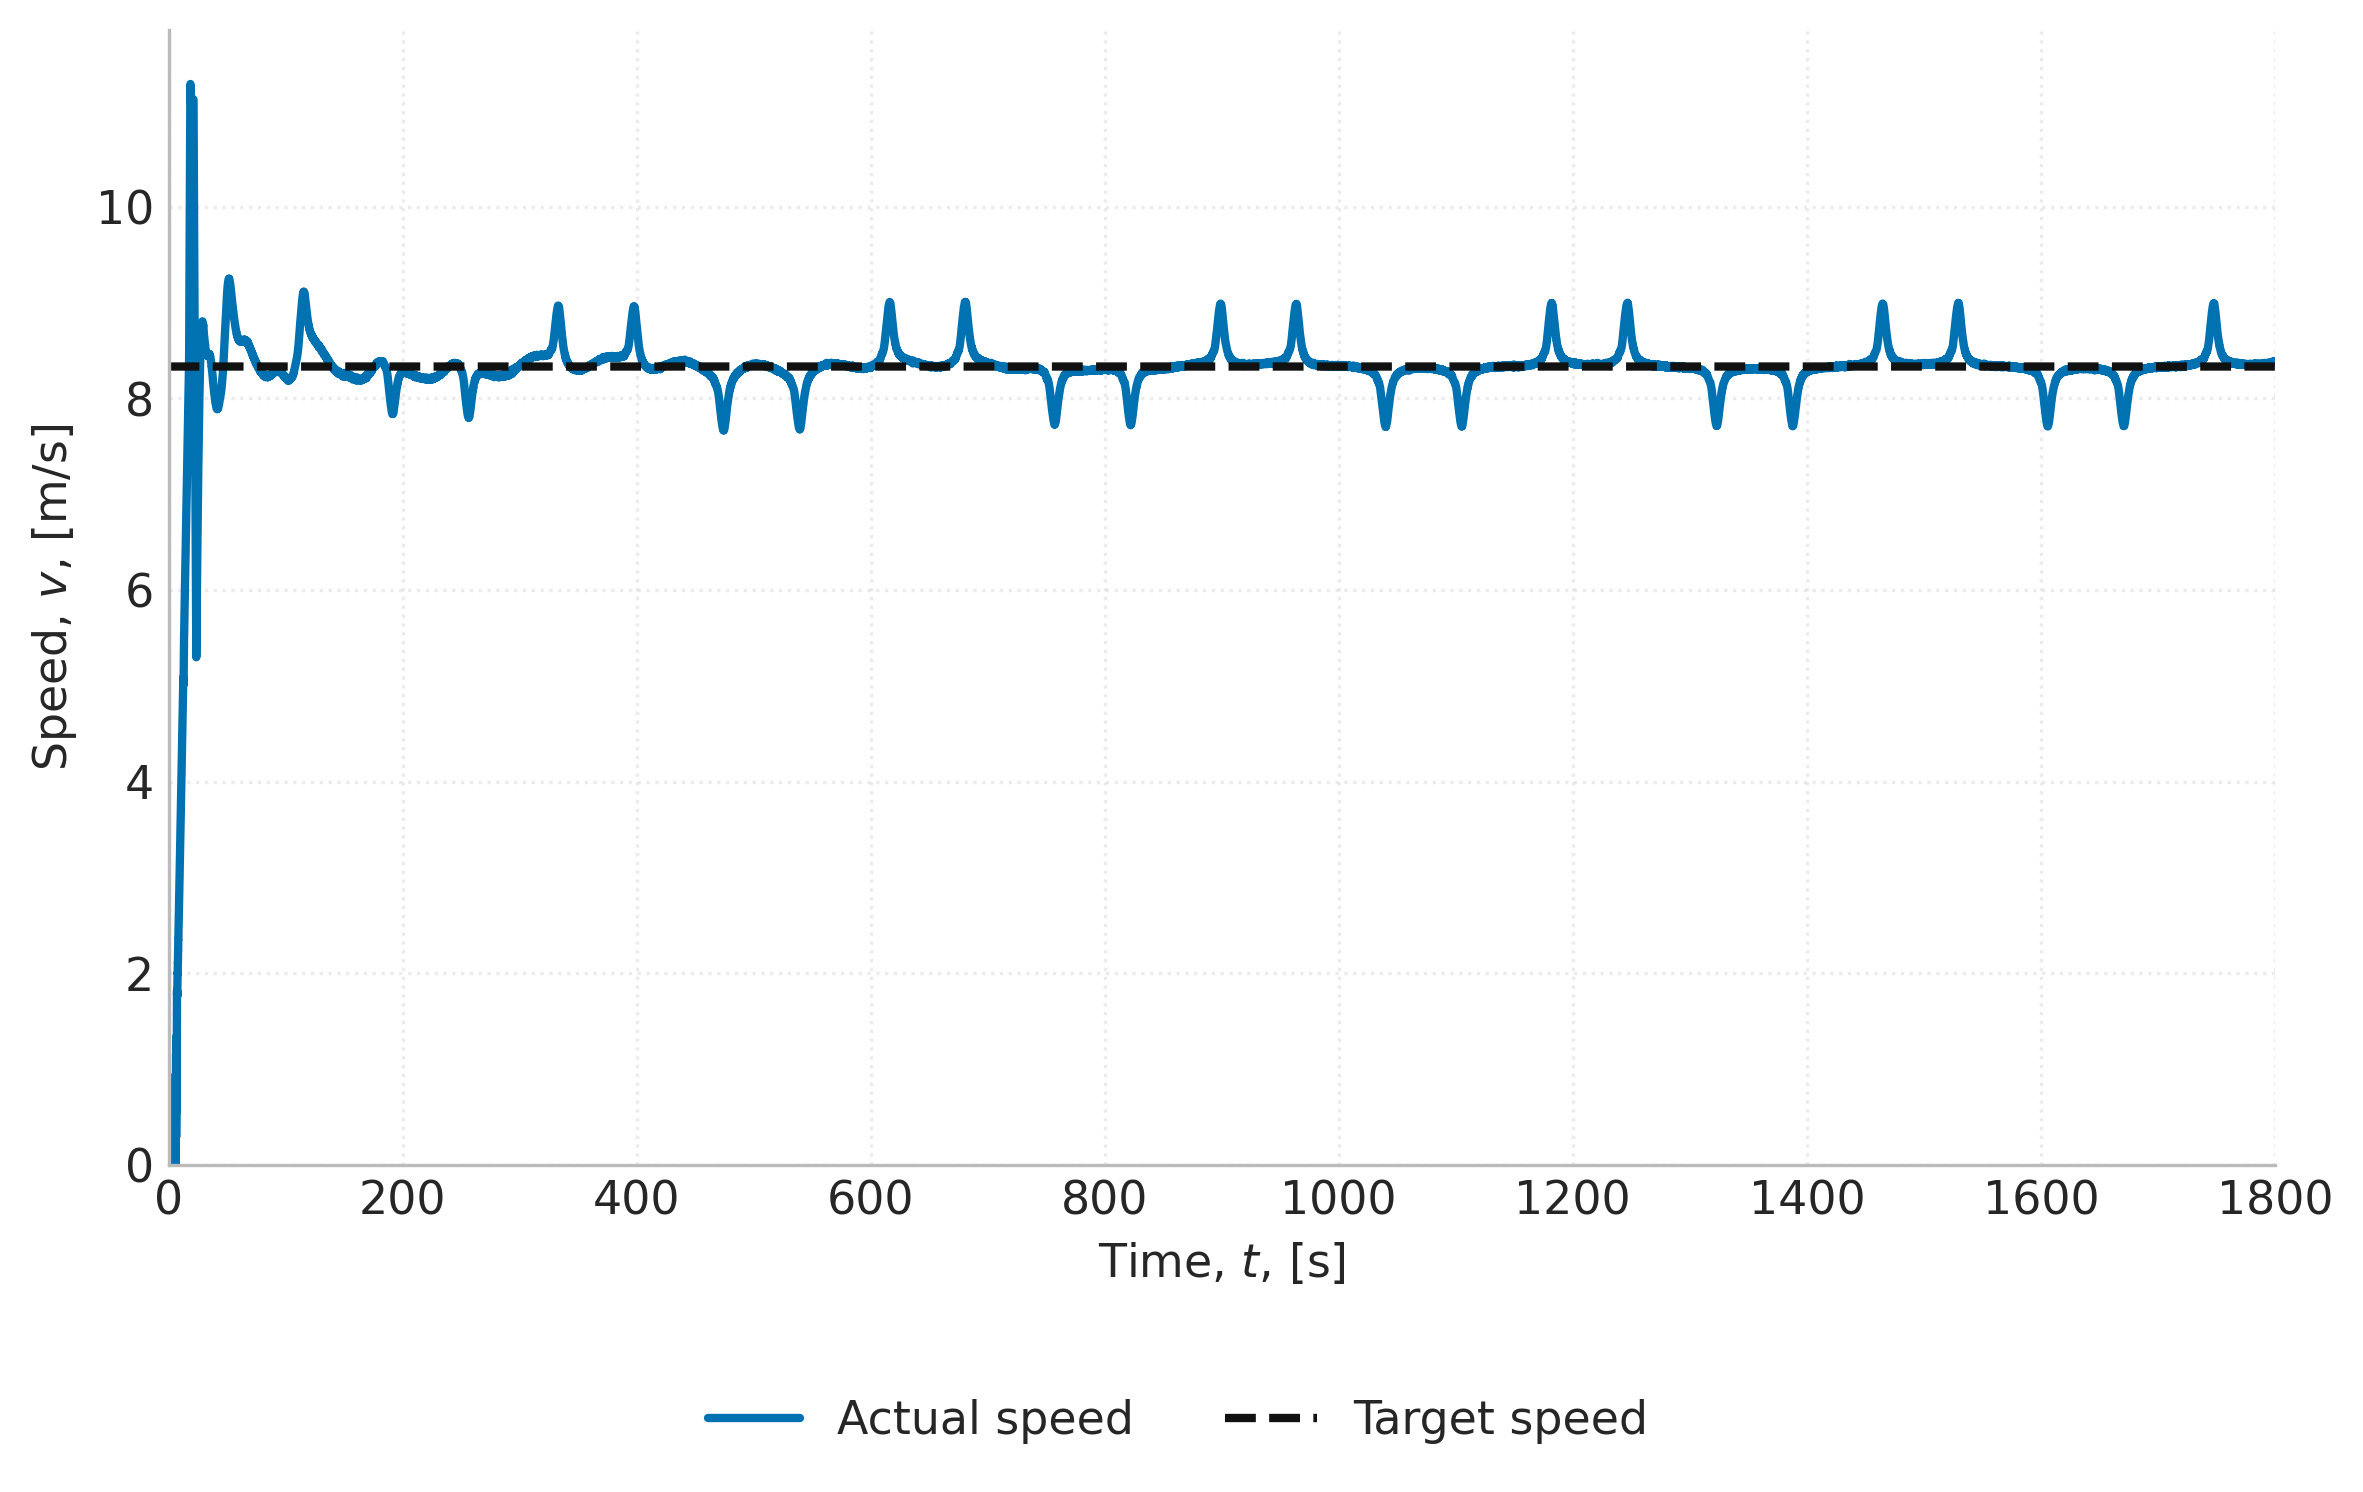
\includegraphics[width=\textwidth]{speed61.png}
        \caption{Speed Profile}
        \label{fig:speed61}
    \end{subfigure}
    \hfill
    \begin{subfigure}[b]{0.48\textwidth}
        \centering
        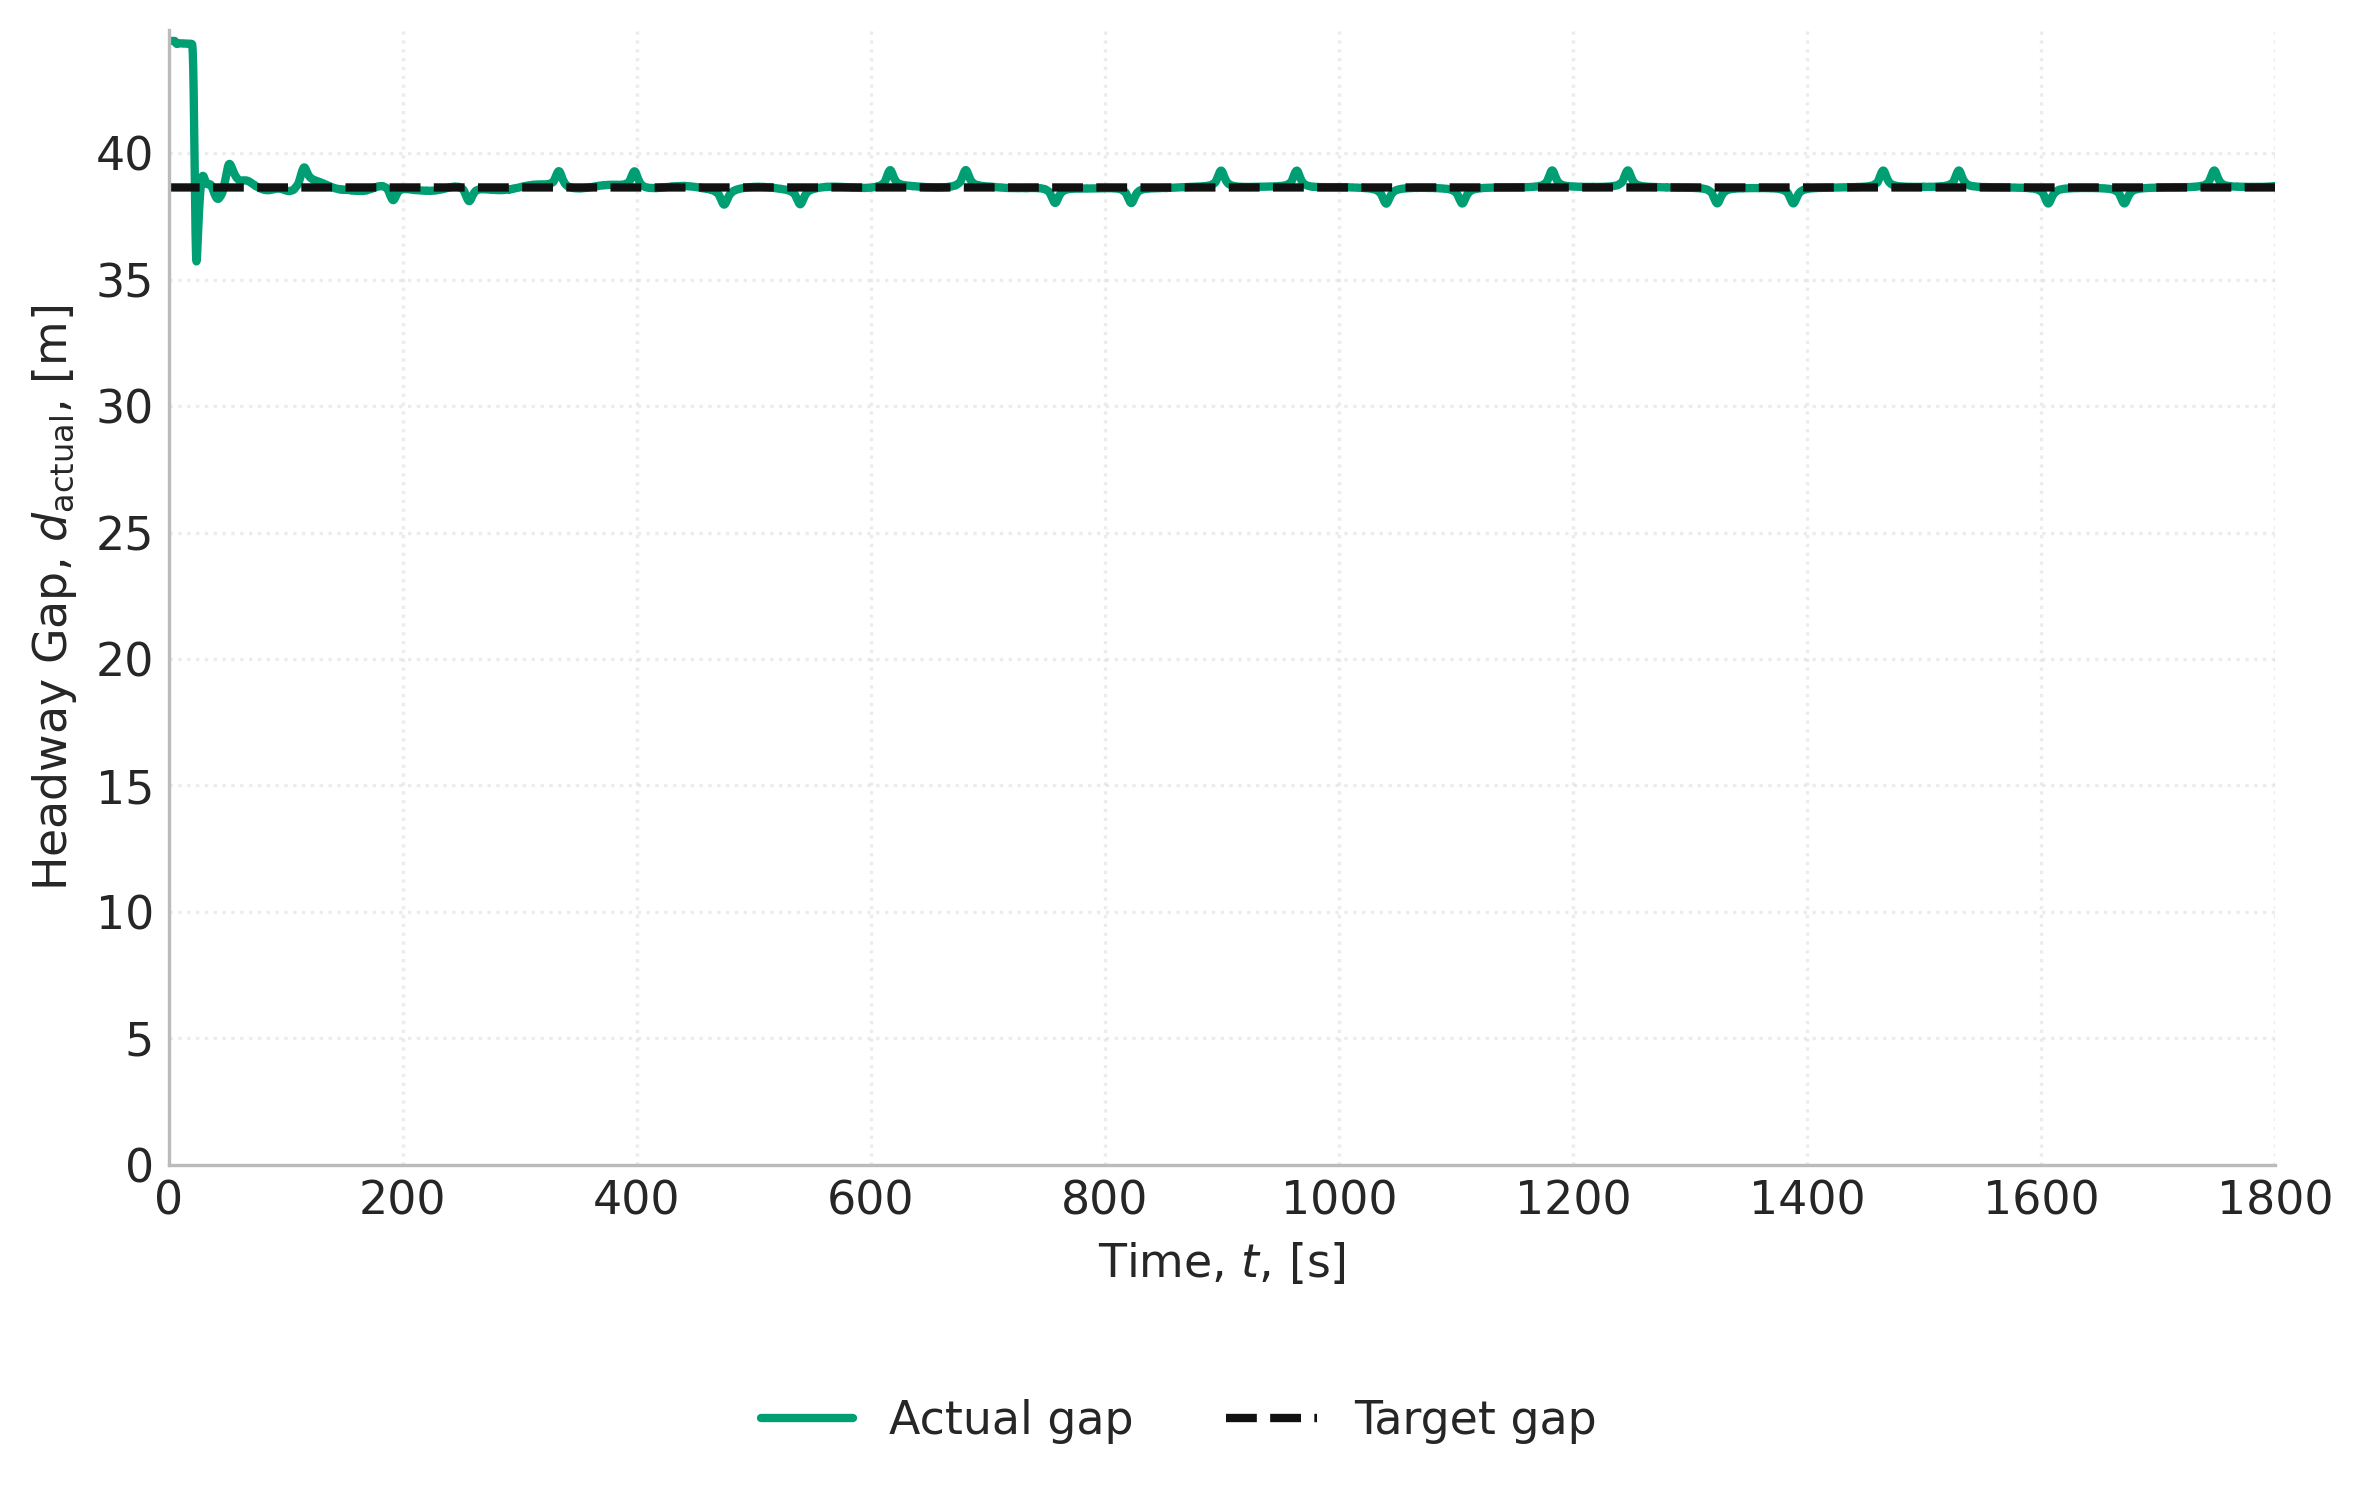
\includegraphics[width=\textwidth]{gap61.png}
        \caption{Gap Distance}
        \label{fig:gap61}
    \end{subfigure}
    
    \vspace{10pt} % Adds vertical spacing between the rows
    \begin{subfigure}[b]{0.48\textwidth}
        \centering
        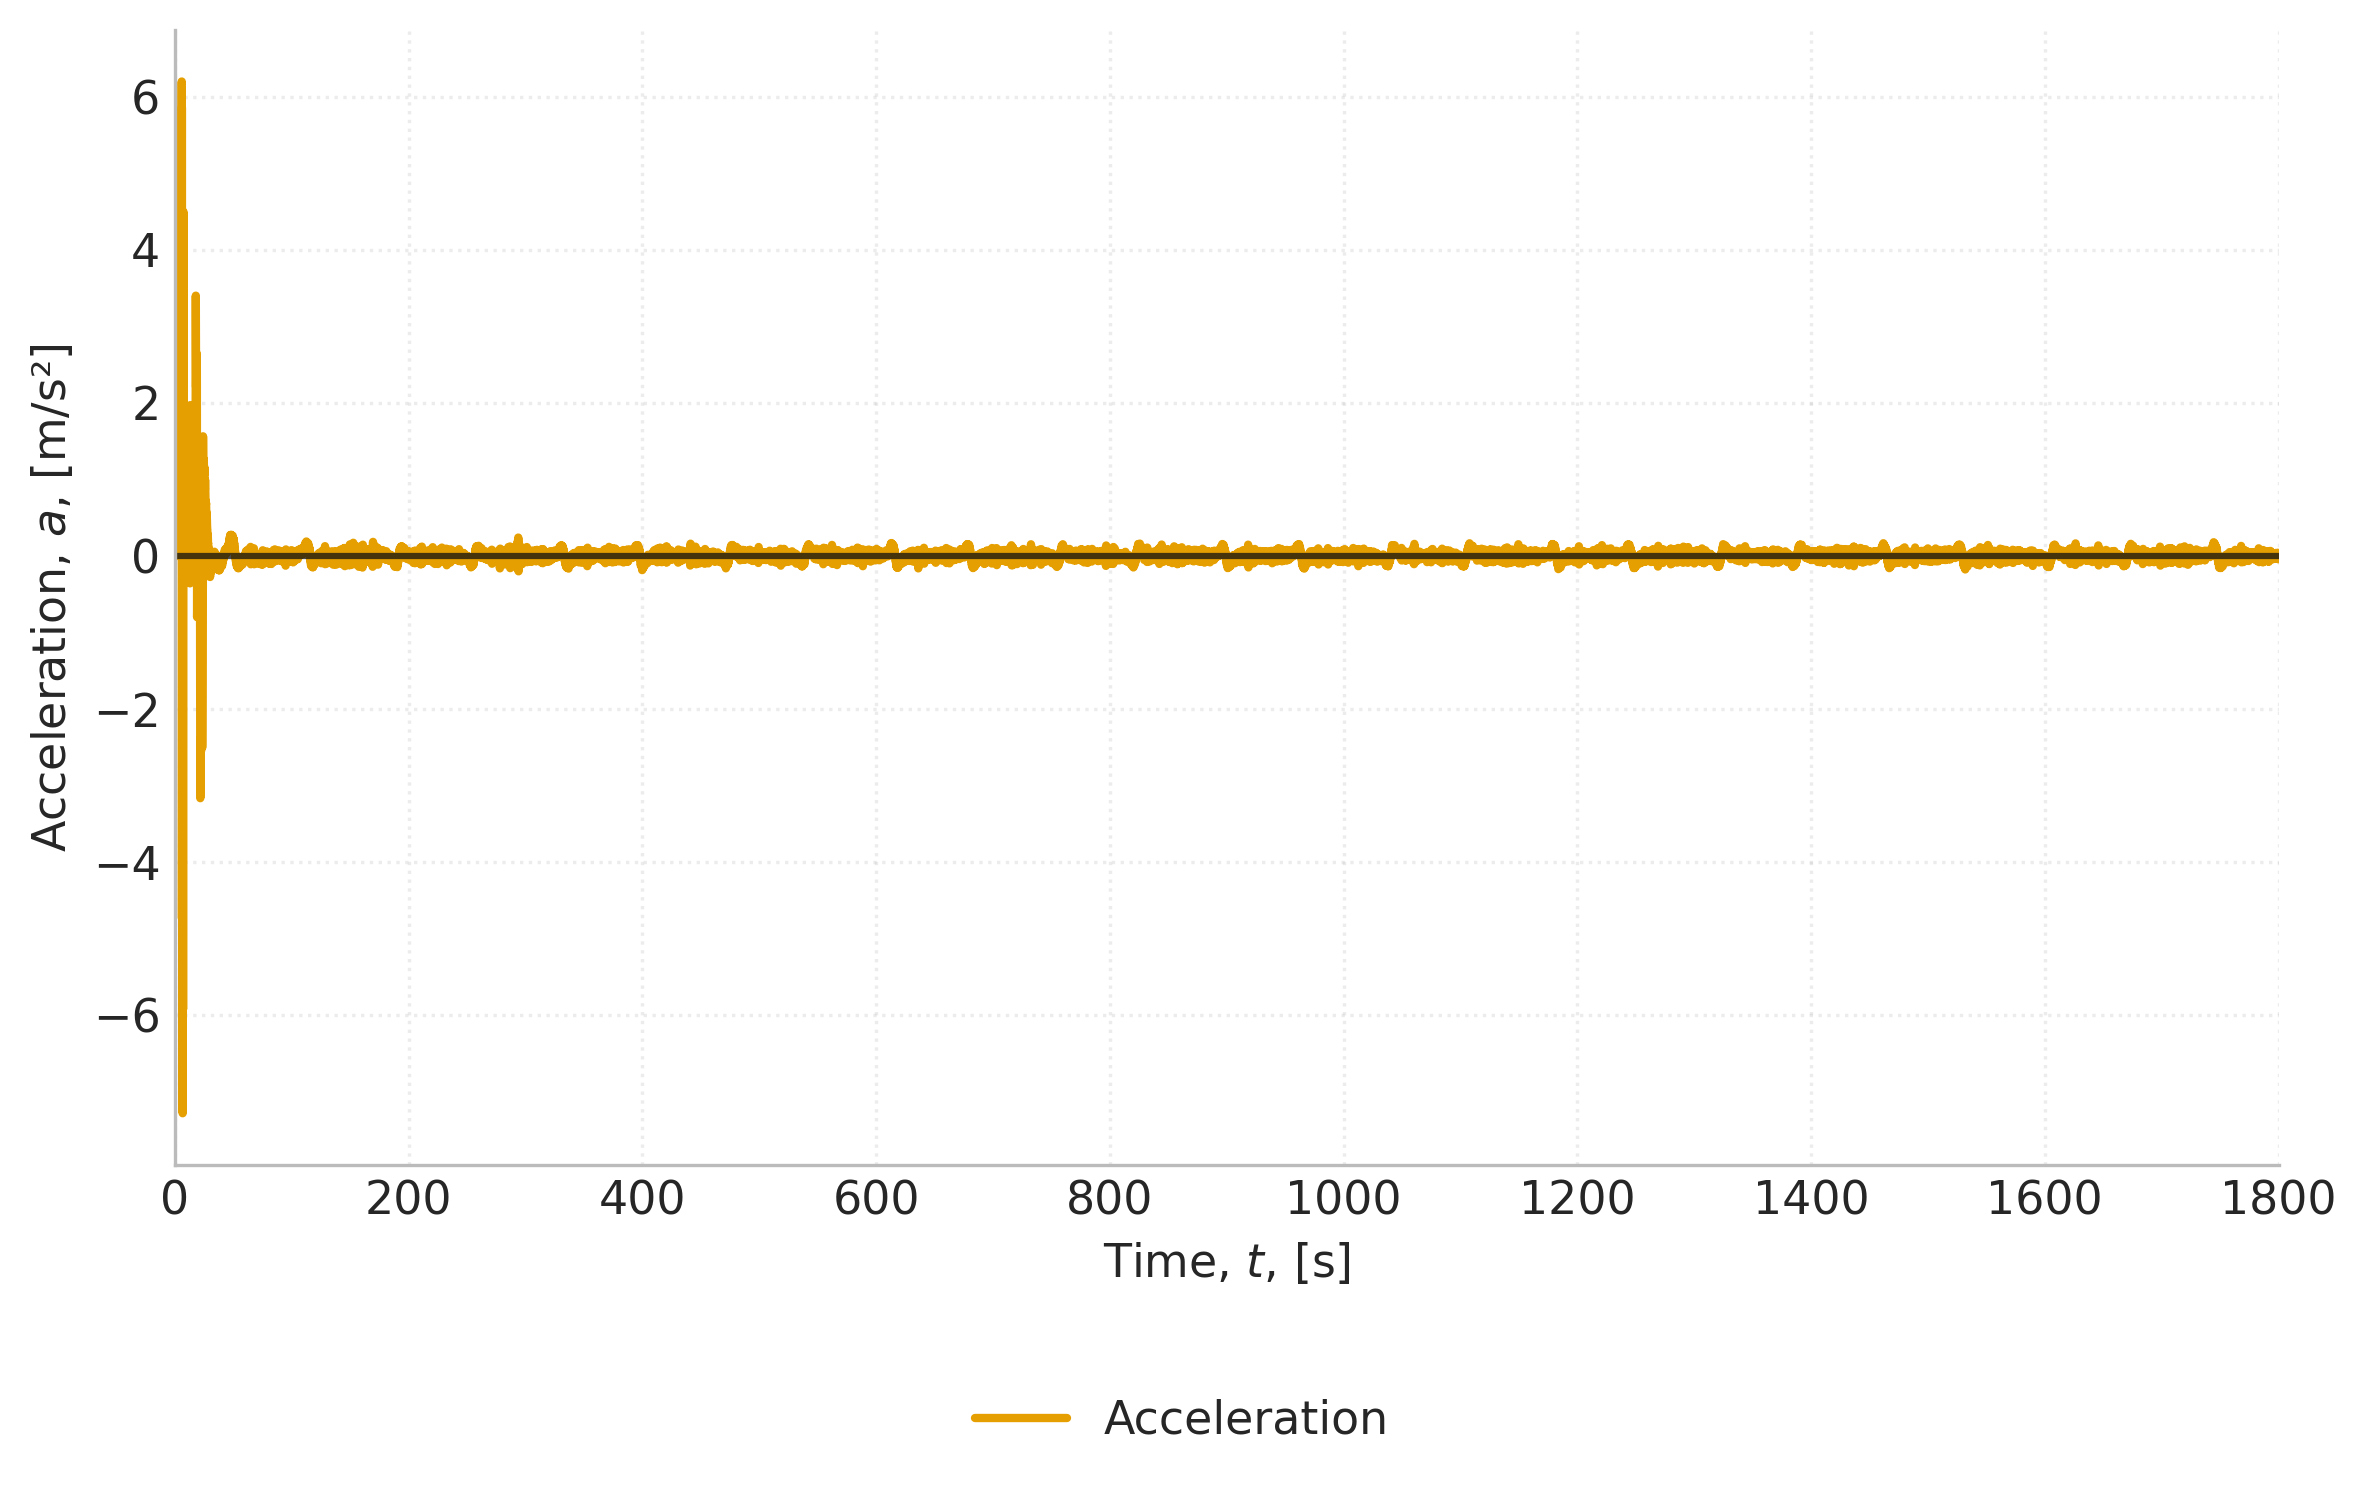
\includegraphics[width=\textwidth]{acceleration61.png}
        \caption{Acceleration Profile}
        \label{fig:accel61}
    \end{subfigure}
    \hfill
    \begin{subfigure}[b]{0.48\textwidth}
        \centering
        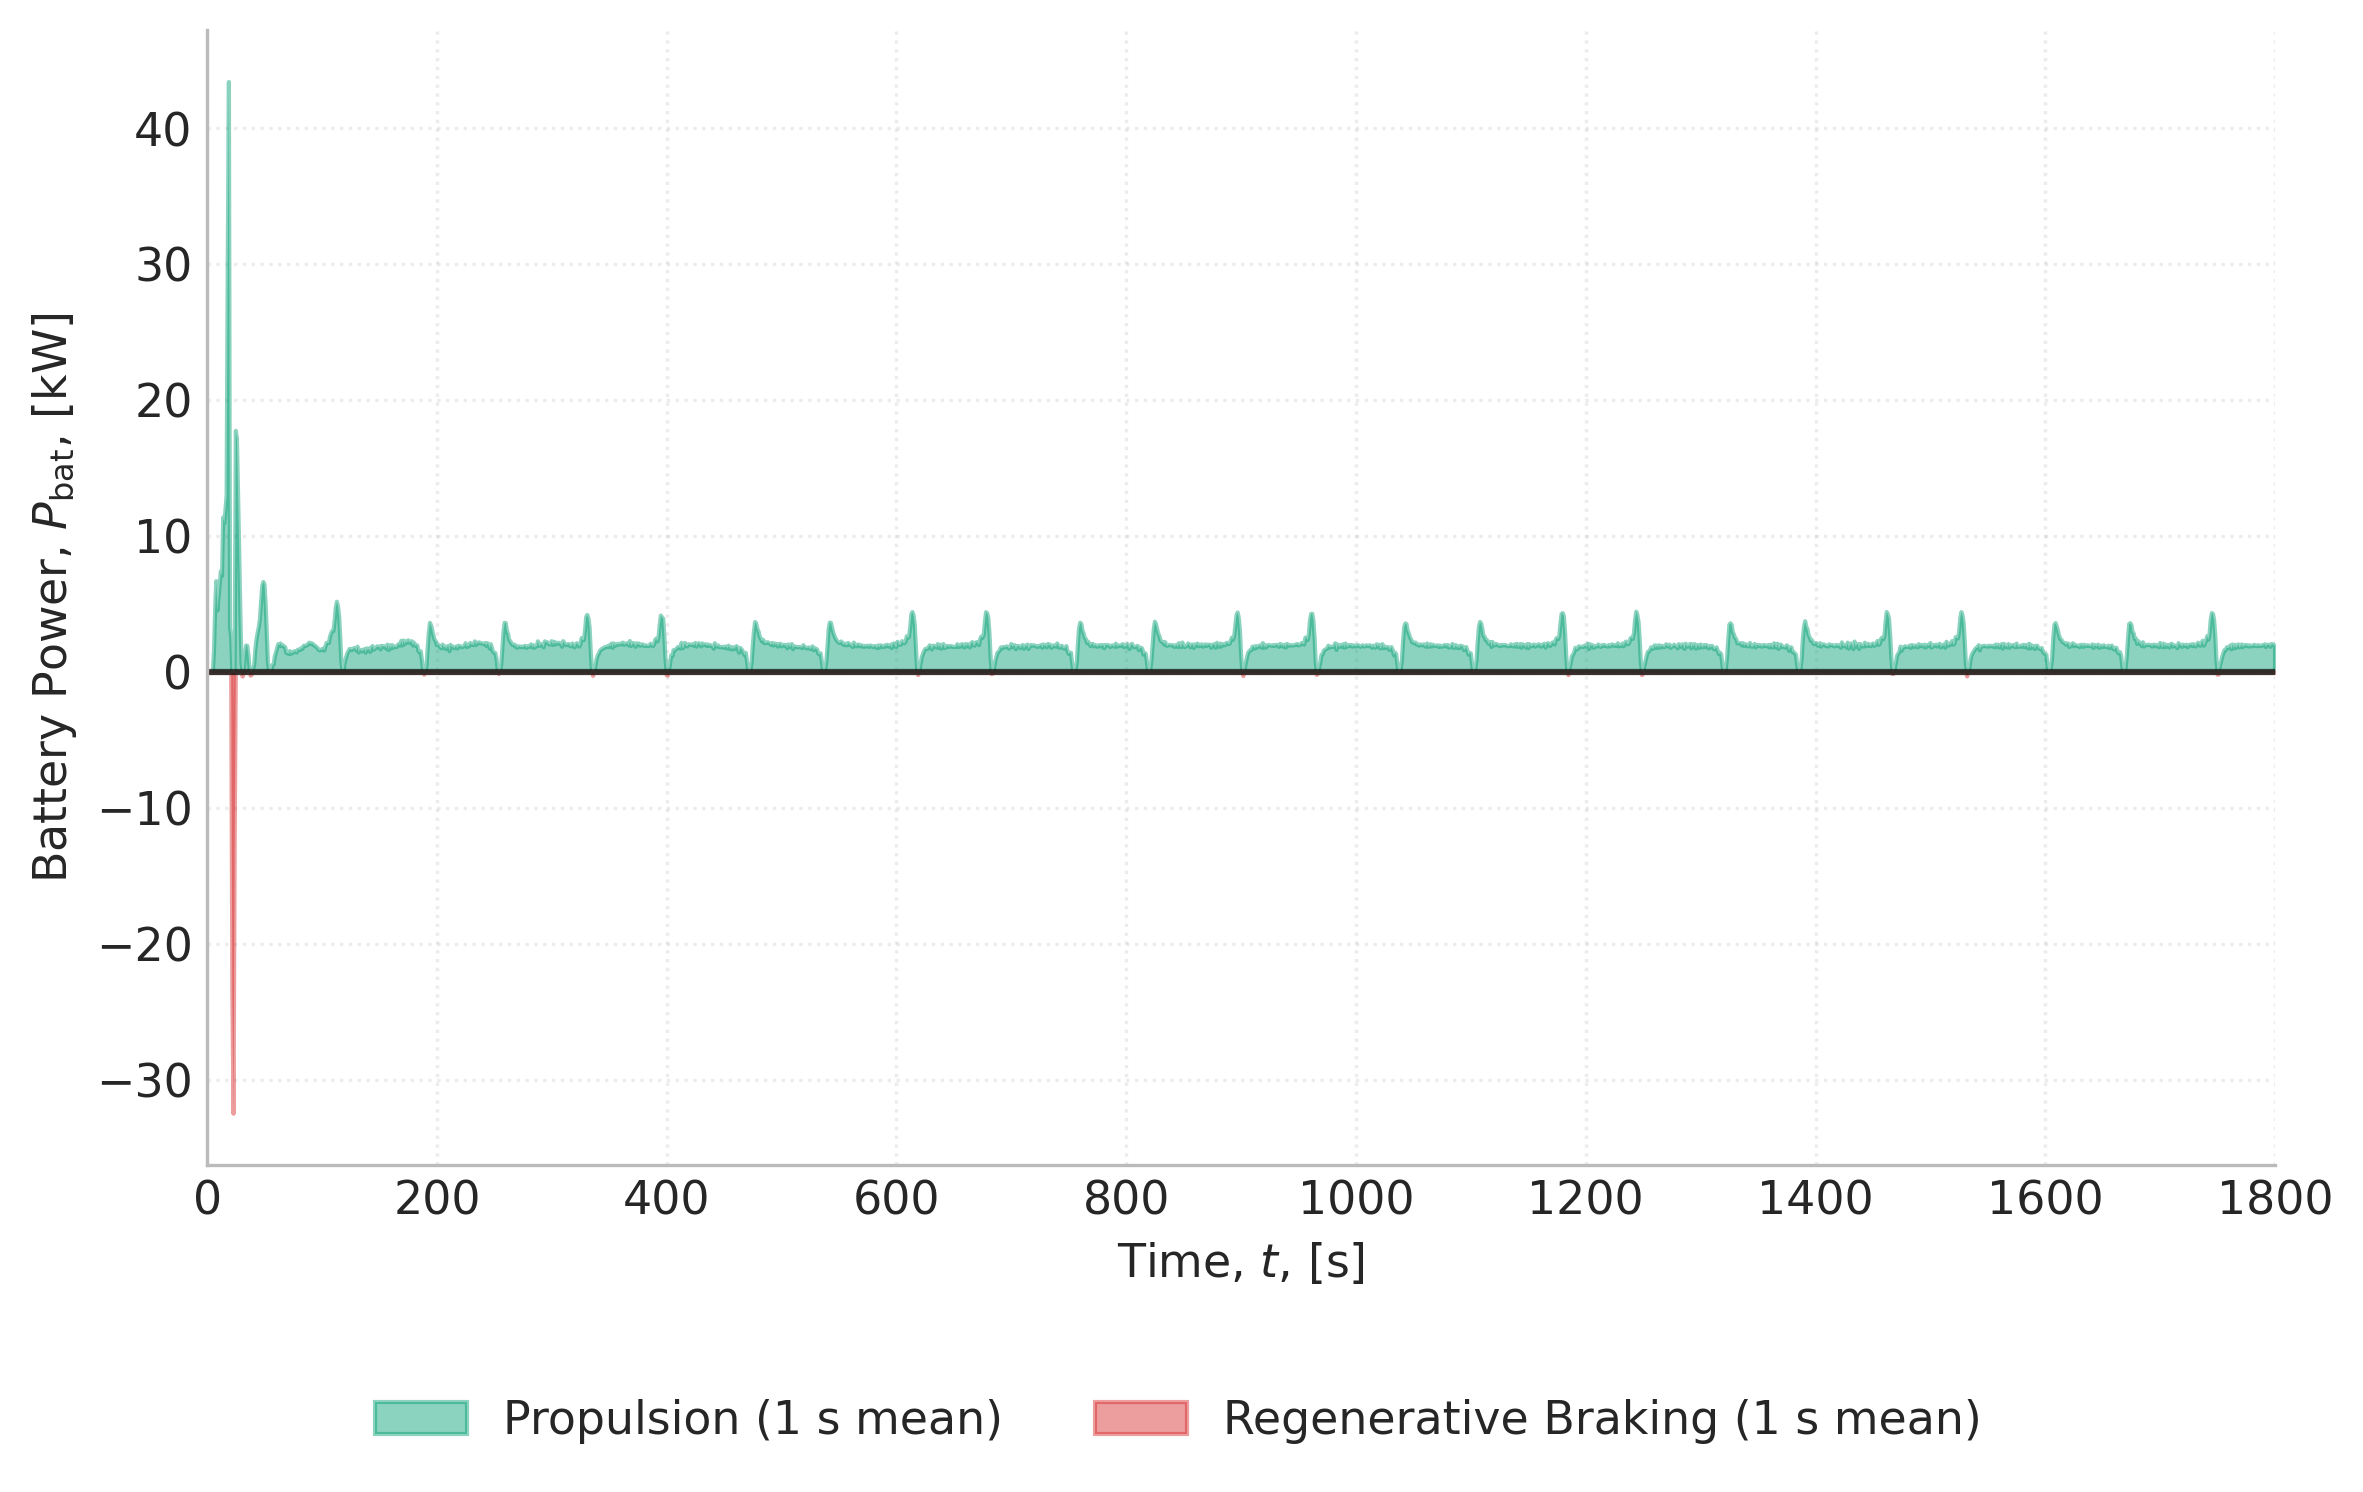
\includegraphics[width=\textwidth]{power61.png}
        \caption{Power Consumption}
        \label{fig:power61}
    \end{subfigure}
    
    \caption{Comprehensive analysis of vehicle metrics for barrier controller; showing acceleration, speed, gap distance, and power consumption for vehicle 1, run 1, and \(N=61\).}
    \label{fig:barrier}
\end{figure}

\subsubsection{FAS Controller Vehicle Behavior}
The vehicle behavior of the FAS controller is illustrated in figure~\ref{fig:fas}, showing accelerations, speed, following gap, and drive power for the same vehicle with identical conditions as described in the previous section.
\\\\
The speed profile, figure~\ref{fig:speed61fas}, shows clear stop-and-go behavior, which can be seen by the actual speed reaching 0, and then increasing again to approximately 11 m/s. The figure also displays that the vehicle often cruises below the target speed at approximately 6 m/s. All in all, it can be seen that the vehicle never cruises at target speed, but rather alters between a complete stop, cruising above the target speed due to large headway gaps after stopping at the traffic light, or cruising below target speed during driving within a queue that has not yet stopped. 
\\\\
The following gap, figure~\ref{fig:gap61fas}, shows that the gap never settles around the target gap, which is in line with the speed profile. The actual gap is either around 6 to 8 m during queuing, or it is above target when the vehicle in front accelerates quickly after a red light due to a large gap error to its predecessor, or it is below target during driving in a queue that has not yet reached a stop. All in all, the FAS controller does not maintain the target spacing, which is expected since vehicles are stopped at the traffic light.
\\\\
The acceleration, section~\ref{fig:acceleration61fas}, also shows stop-and-go behavior, characterized by large accelerations and decelerations. With respect to the latter, it can be seen that the vehicle decelerates at -7.5 \(m/s^2\), which is far more aggressive than a comfortable deceleration of 2.5 \(m/s^2\) \parencite{carlowitz2026balancing}. 
\\\\
Drive power, figure~\ref{fig:power61fas}, illustrates propulsion peaks during acceleration peaks, and regenerative braking peaks during deceleration peaks.  
\\\\
In general, the FAS controller exhibits erratic behavior. Instead of cruising smoothly at all targets, the vehicle shows clear stop-and-go behavior, resulting in deviation from both target gap and target speed, large accelerations and decelerations, and switching between propulsion and regenerative braking. 




\begin{figure}[H]
    \centering
    \begin{subfigure}[b]{0.48\textwidth}
        \centering
        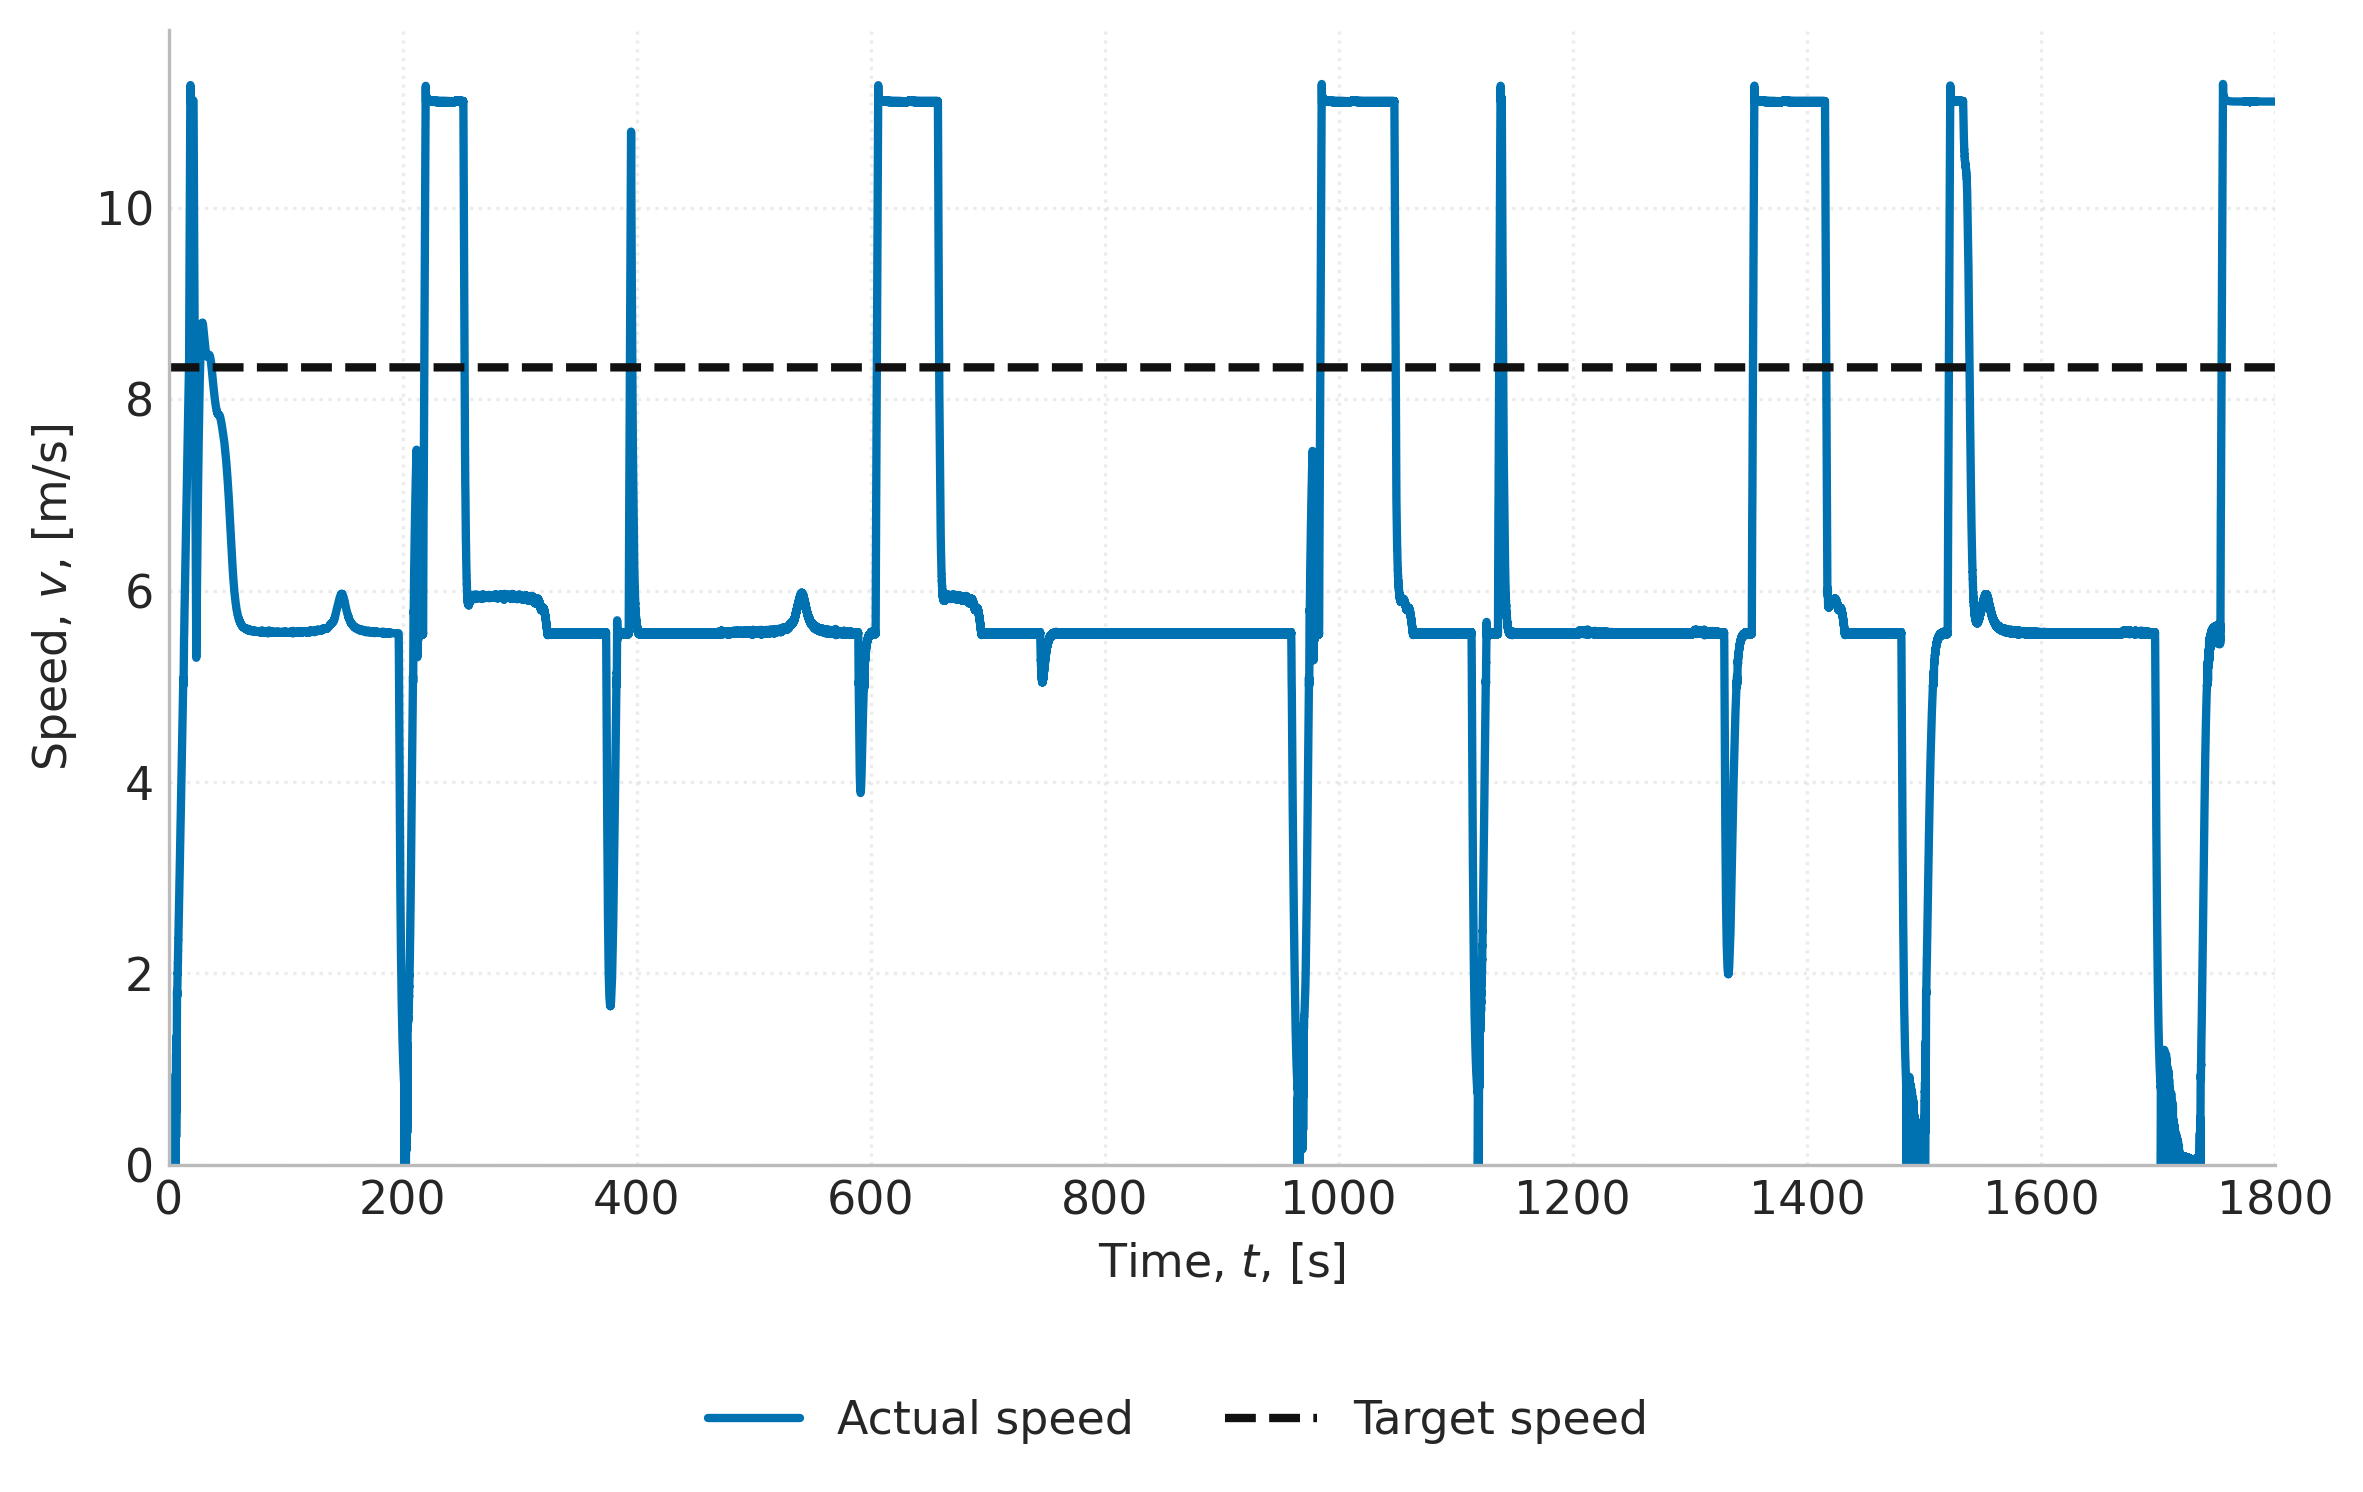
\includegraphics[width=\textwidth]{speed61fas.png}
        \caption{Speed Profile}
        \label{fig:speed61fas}
    \end{subfigure}
    \hfill
    \begin{subfigure}[b]{0.48\textwidth}
        \centering
        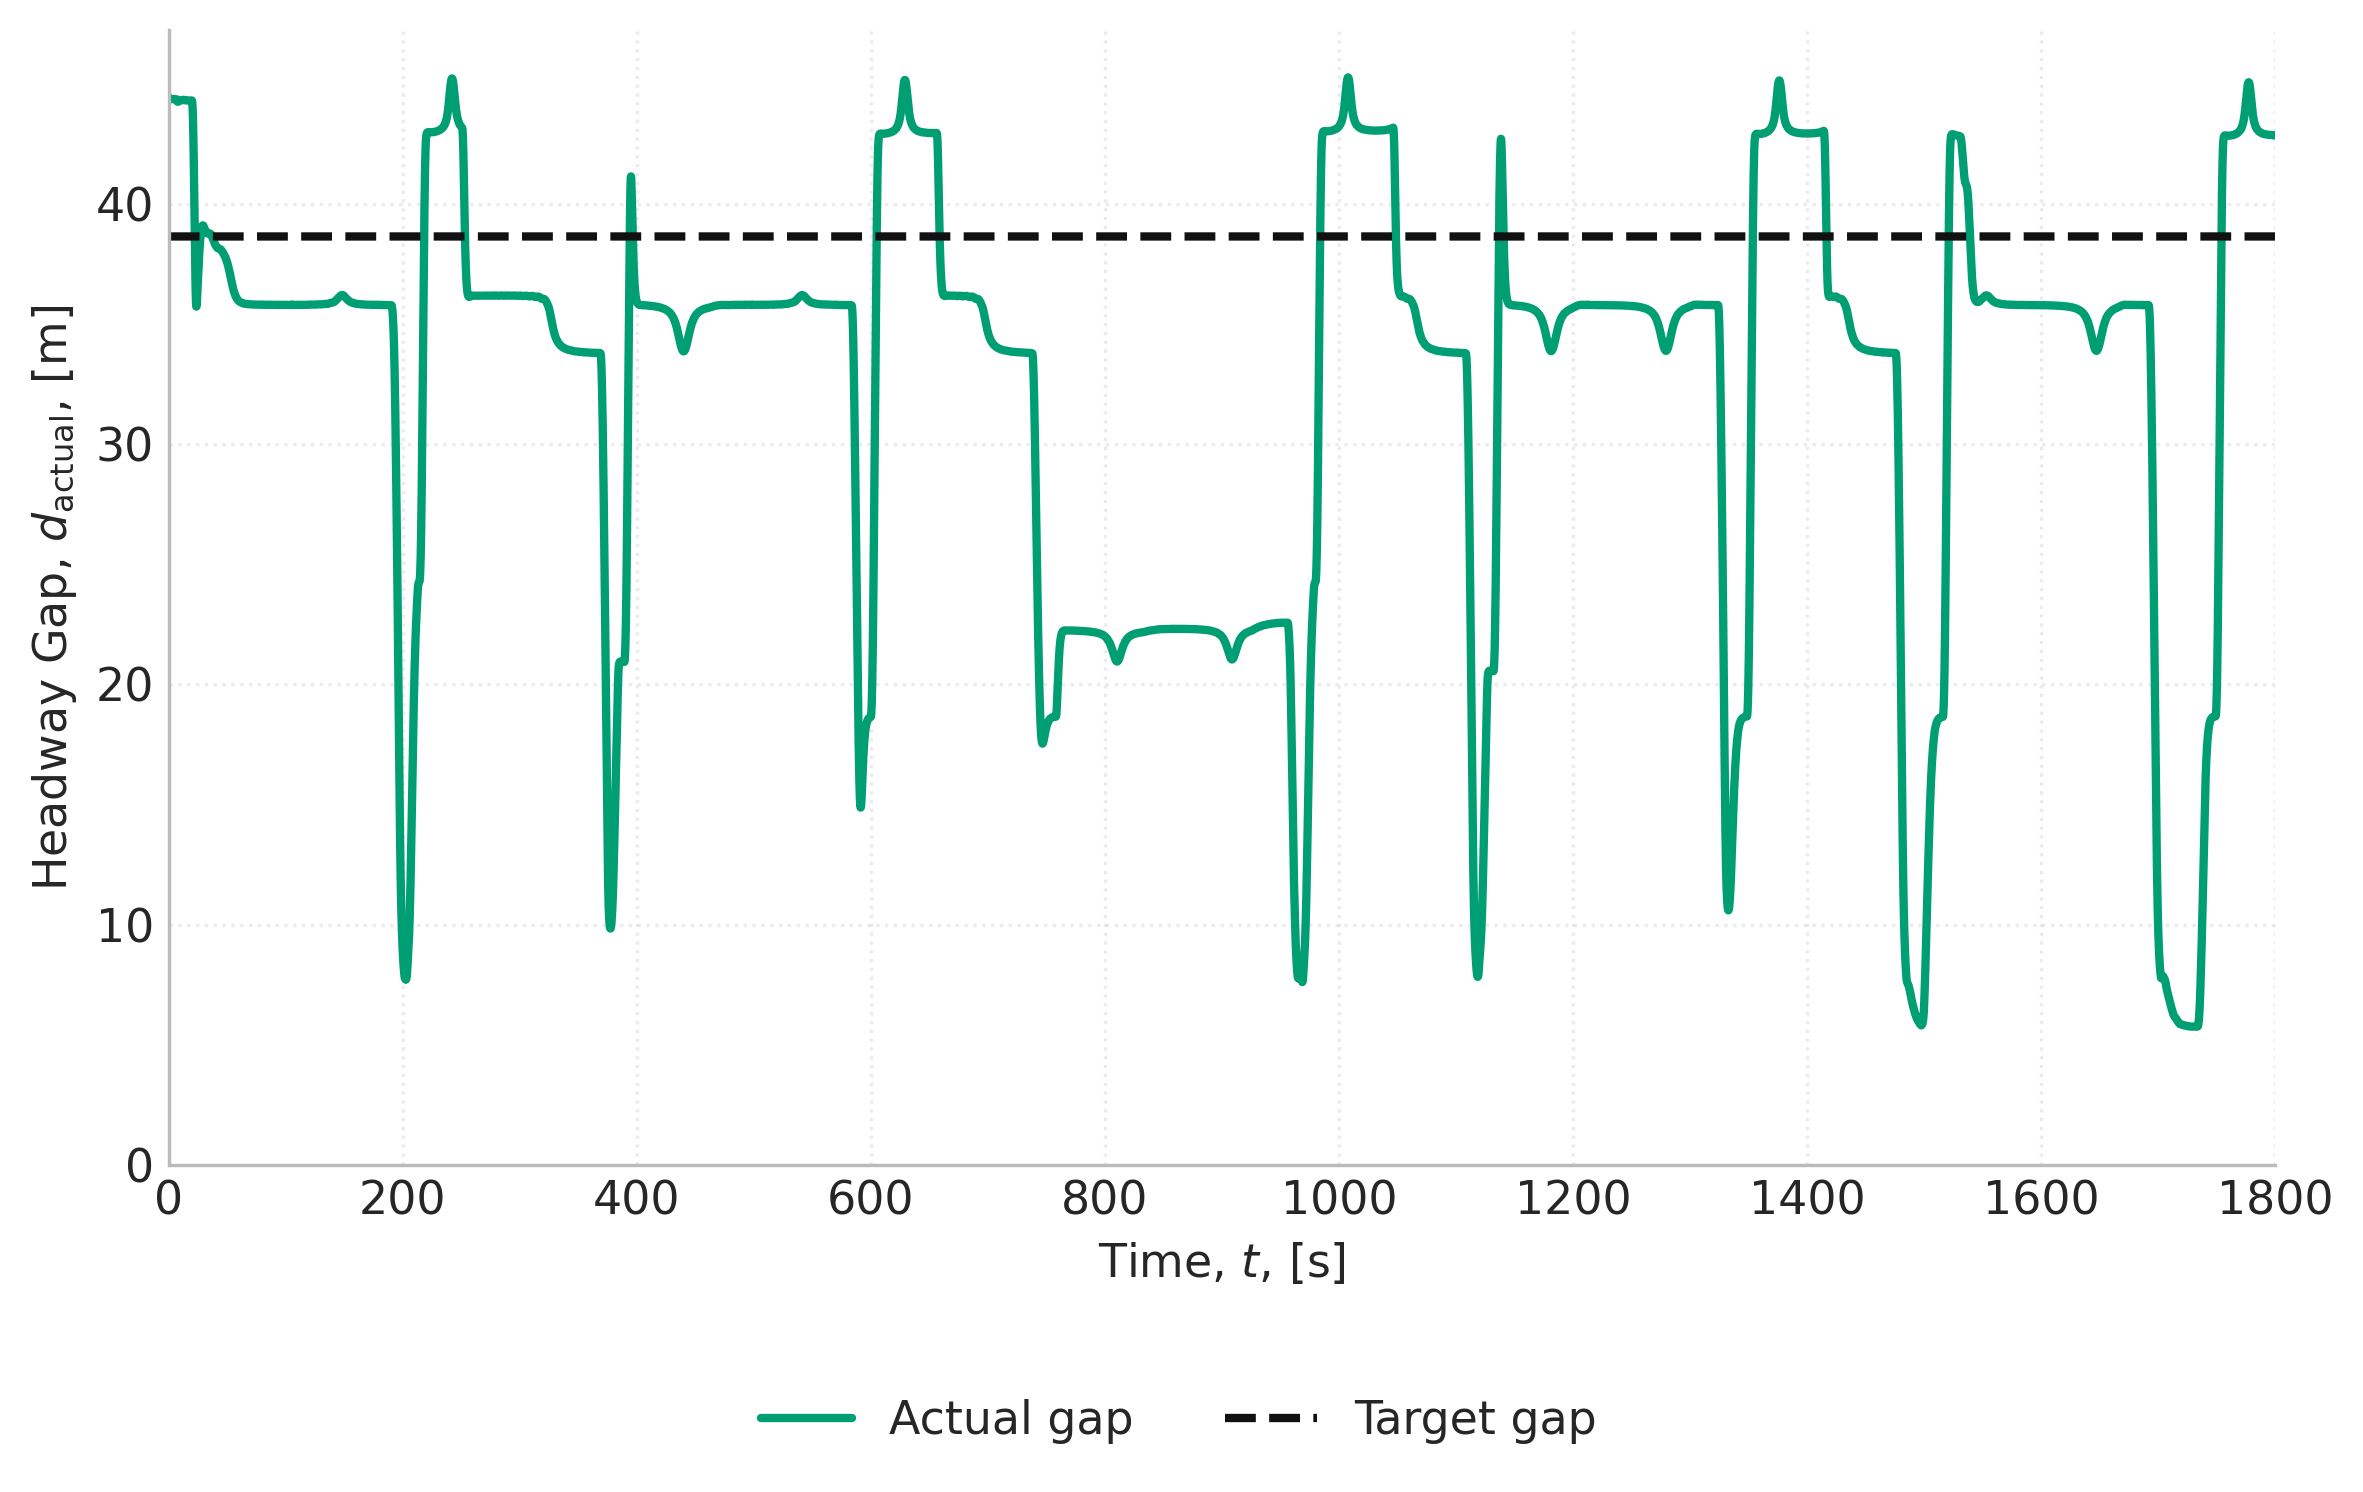
\includegraphics[width=\textwidth]{gap61fas.png}
        \caption{Gap Distance}
        \label{fig:gap61fas}
    \end{subfigure}
    
    \vspace{10pt} % Adds vertical spacing between the rows
     \begin{subfigure}[b]{0.48\textwidth}
        \centering
        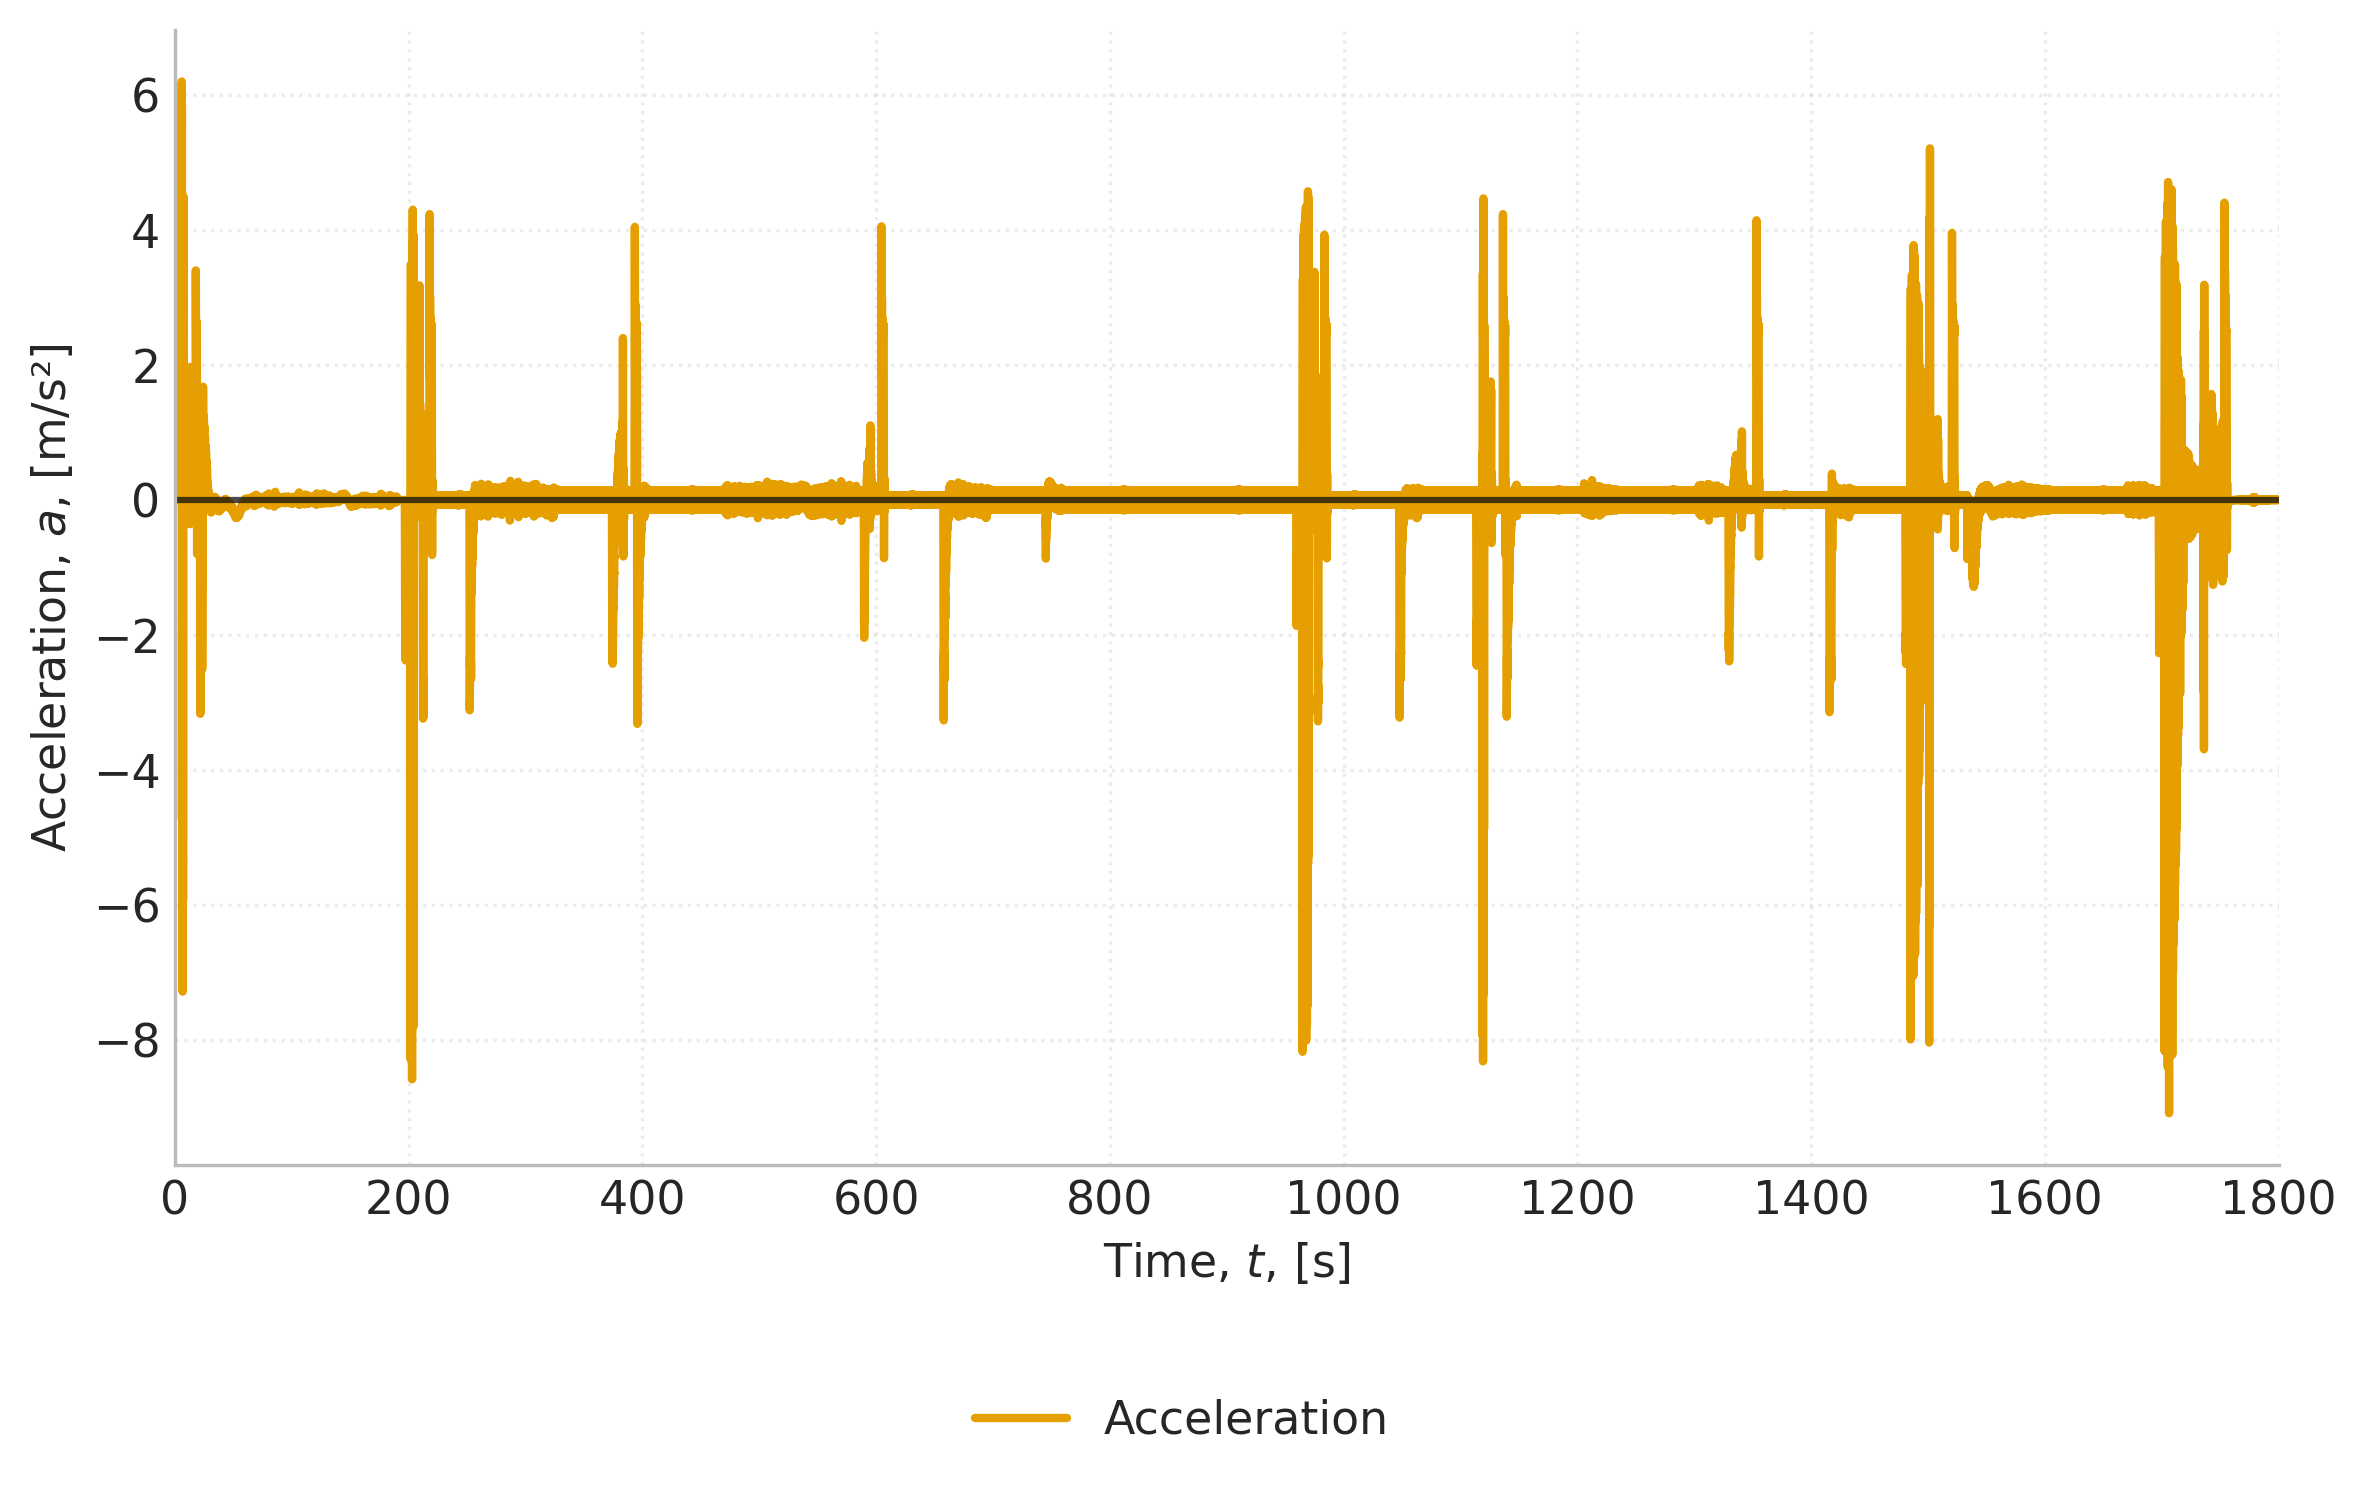
\includegraphics[width=\textwidth]{acceleration61fas.png}
        \caption{Acceleration Profile}
        \label{fig:acceleration61fas}
    \end{subfigure}
    \hfill
    \begin{subfigure}[b]{0.48\textwidth}
        \centering
        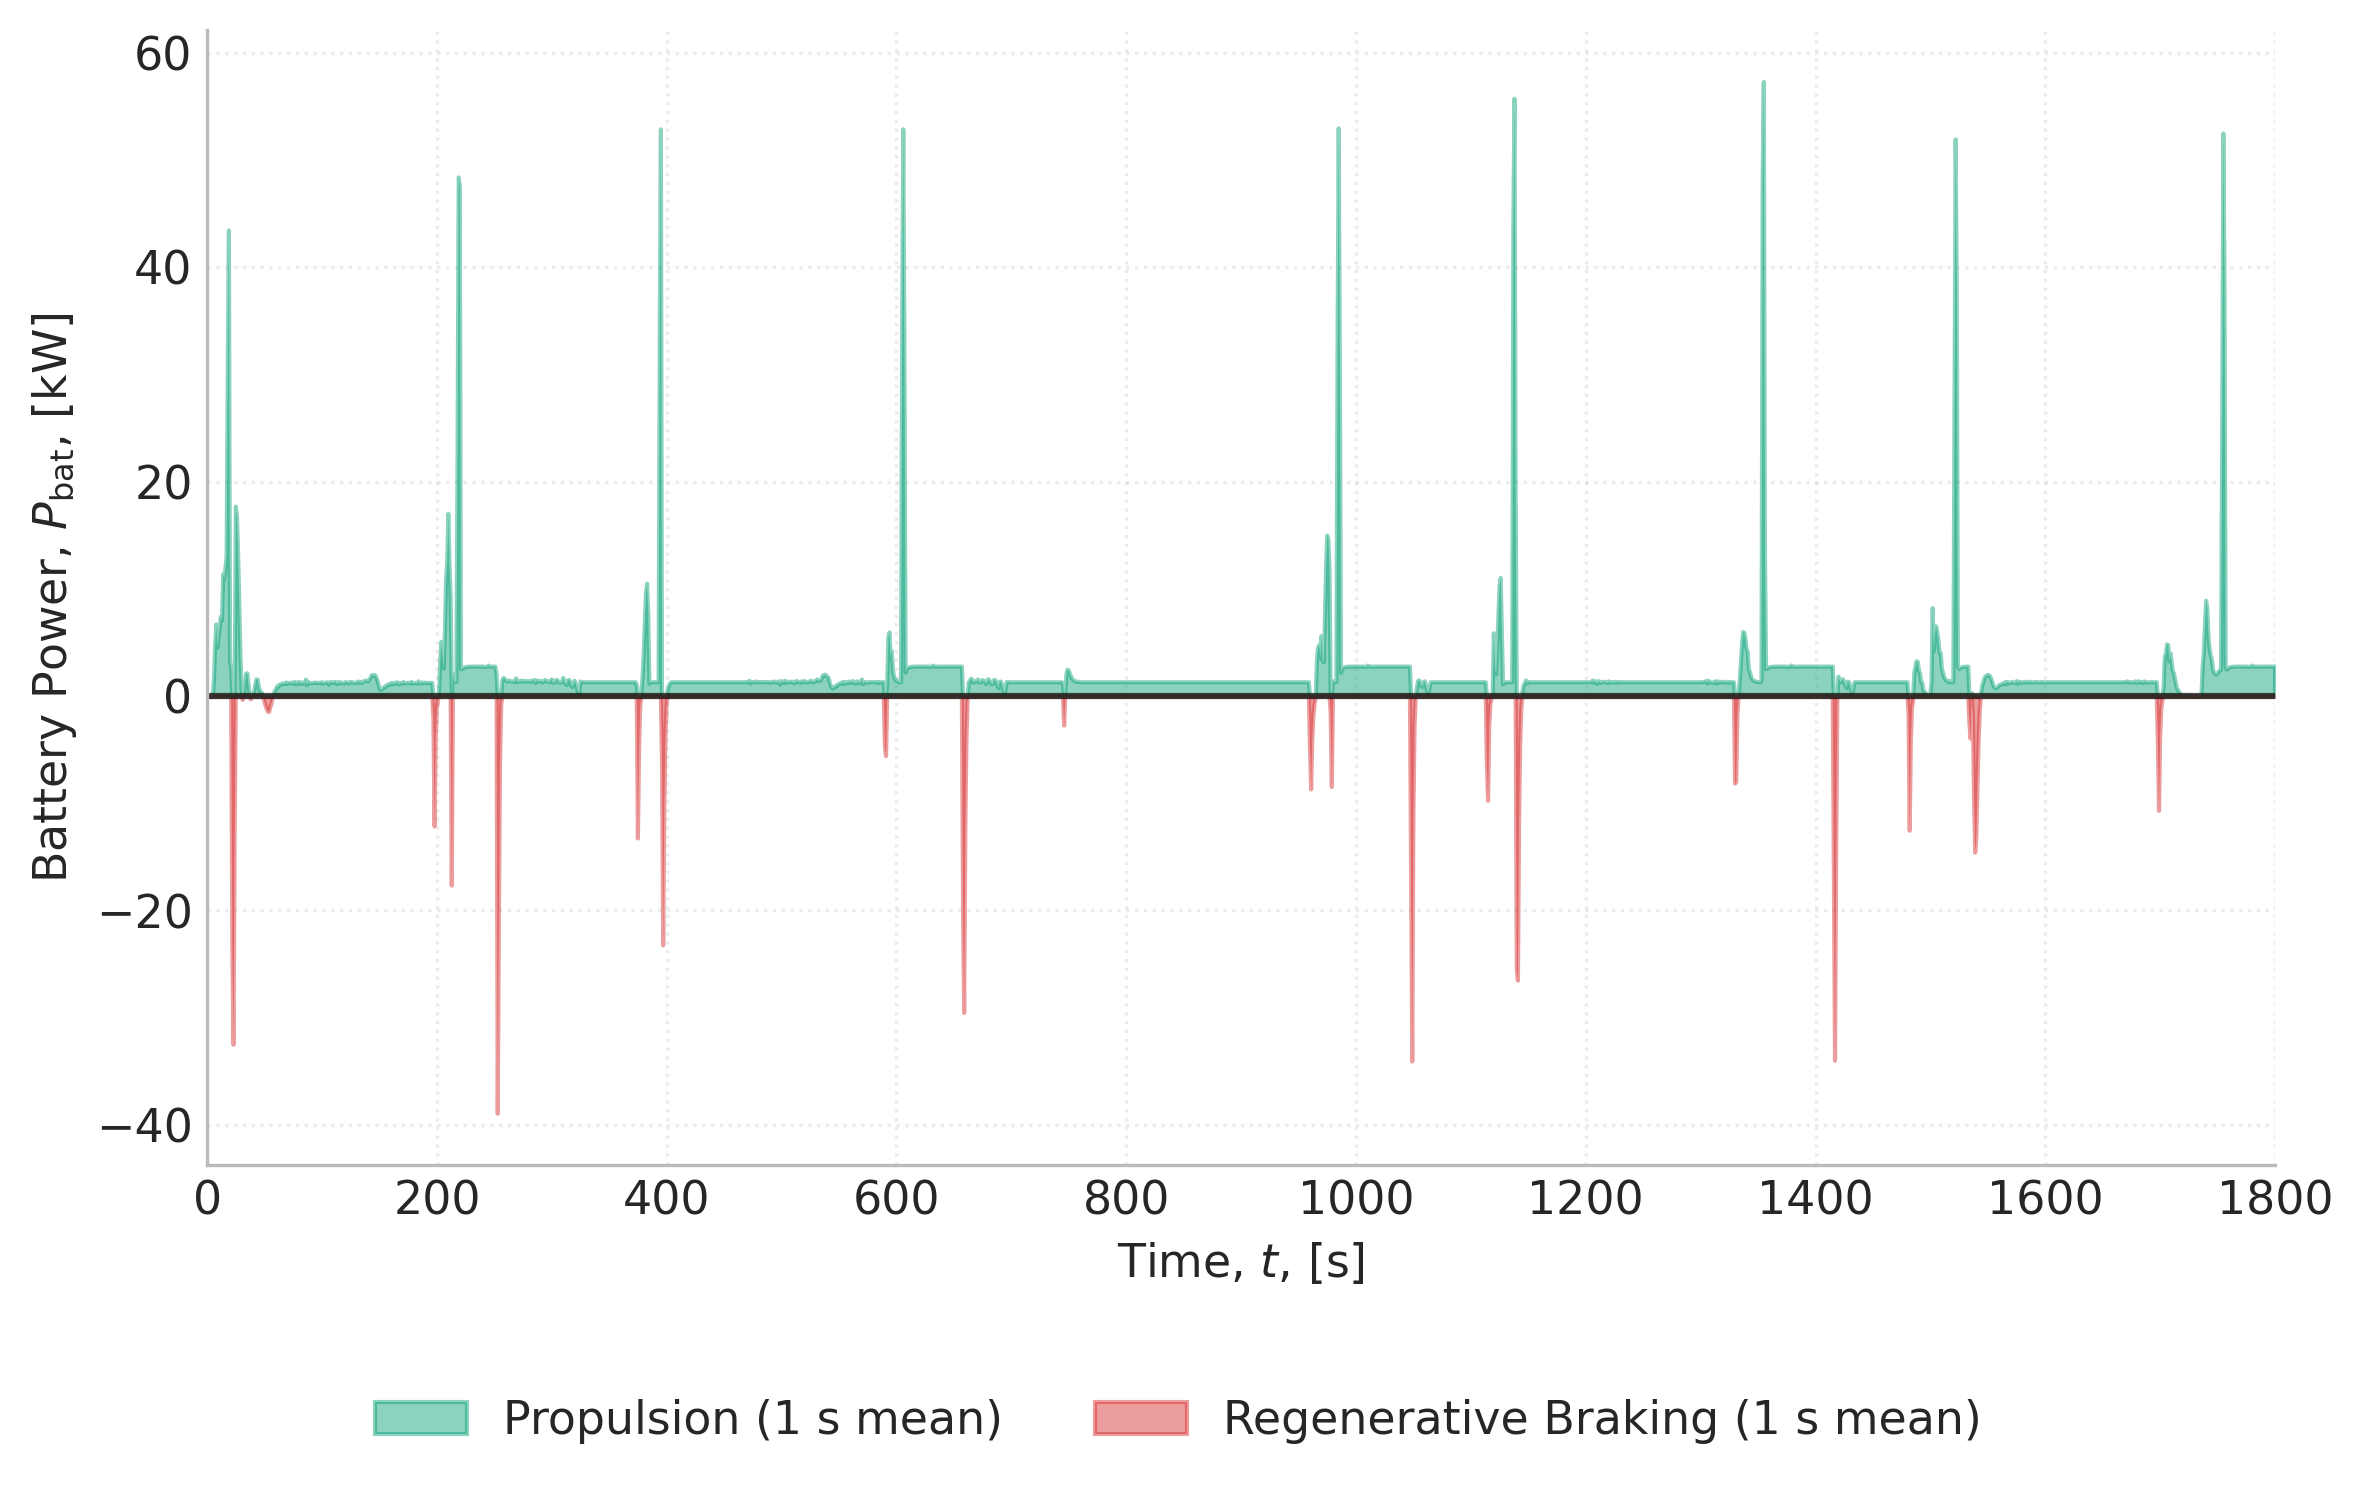
\includegraphics[width=\textwidth]{power61fas.png}
        \caption{Power Consumption}
        \label{fig:power61fas}
    \end{subfigure}
    
    \caption{Comprehensive analysis of vehicle metrics for FAS controller; showing acceleration, speed, gap distance, and power profiles for vehicle 1, run 1, and \(N=61\).}
    \label{fig:fas}
\end{figure}

\subsection{Barrier Controller Performance}
The performance of the barrier controller is verified, in terms of activations across the various vehicle counts. Figure~\ref{fig:firings-per-demand}, shows a box-plot of the number of barrier controller activations per batch. The figure highlights, that the barrier activates more often at a higher vehicle density. At \(N=51\) vehicles, the barrier never activates across all runs. Similar behavior is seen at \(N=61\), where the barrier fired a small amount of times. From \(N=71\), the barrier fires on average 18 times, with some simulation runs without firings, highlighted by the whisker reaching 0, and some extreme scenarios of 40 firings. For \(N=81\), the barrier fired on average 153 times, with extreme scenarios of almost 175 firings, and some scenarios with around 105 firings. Figure~\ref{fig:firings-over-time} reveals that the barrier fires until it reaches a so called steady state, which is the state where the vehicles are moving at their target gap and form a platoon. The platoon forms in a manner which ensures no barrier activations are required to cross the conflict point. In addition, the figure also reveals that for \(N=71\), this platoon forming and spacing happens within 200 s, whereas for \(N=81\) the movement requires more time and is reached within approximately 550 s. This confirms that the barrier correctly handles varying vehicle densities and is able to drive the vehicles to a steady-state platoon.

\begin{figure}[htbp]
    \centering
    \begin{subfigure}[b]{0.48\textwidth}
        \centering
        % Scaled by height (e.g., 4cm), aspect ratio preserved
        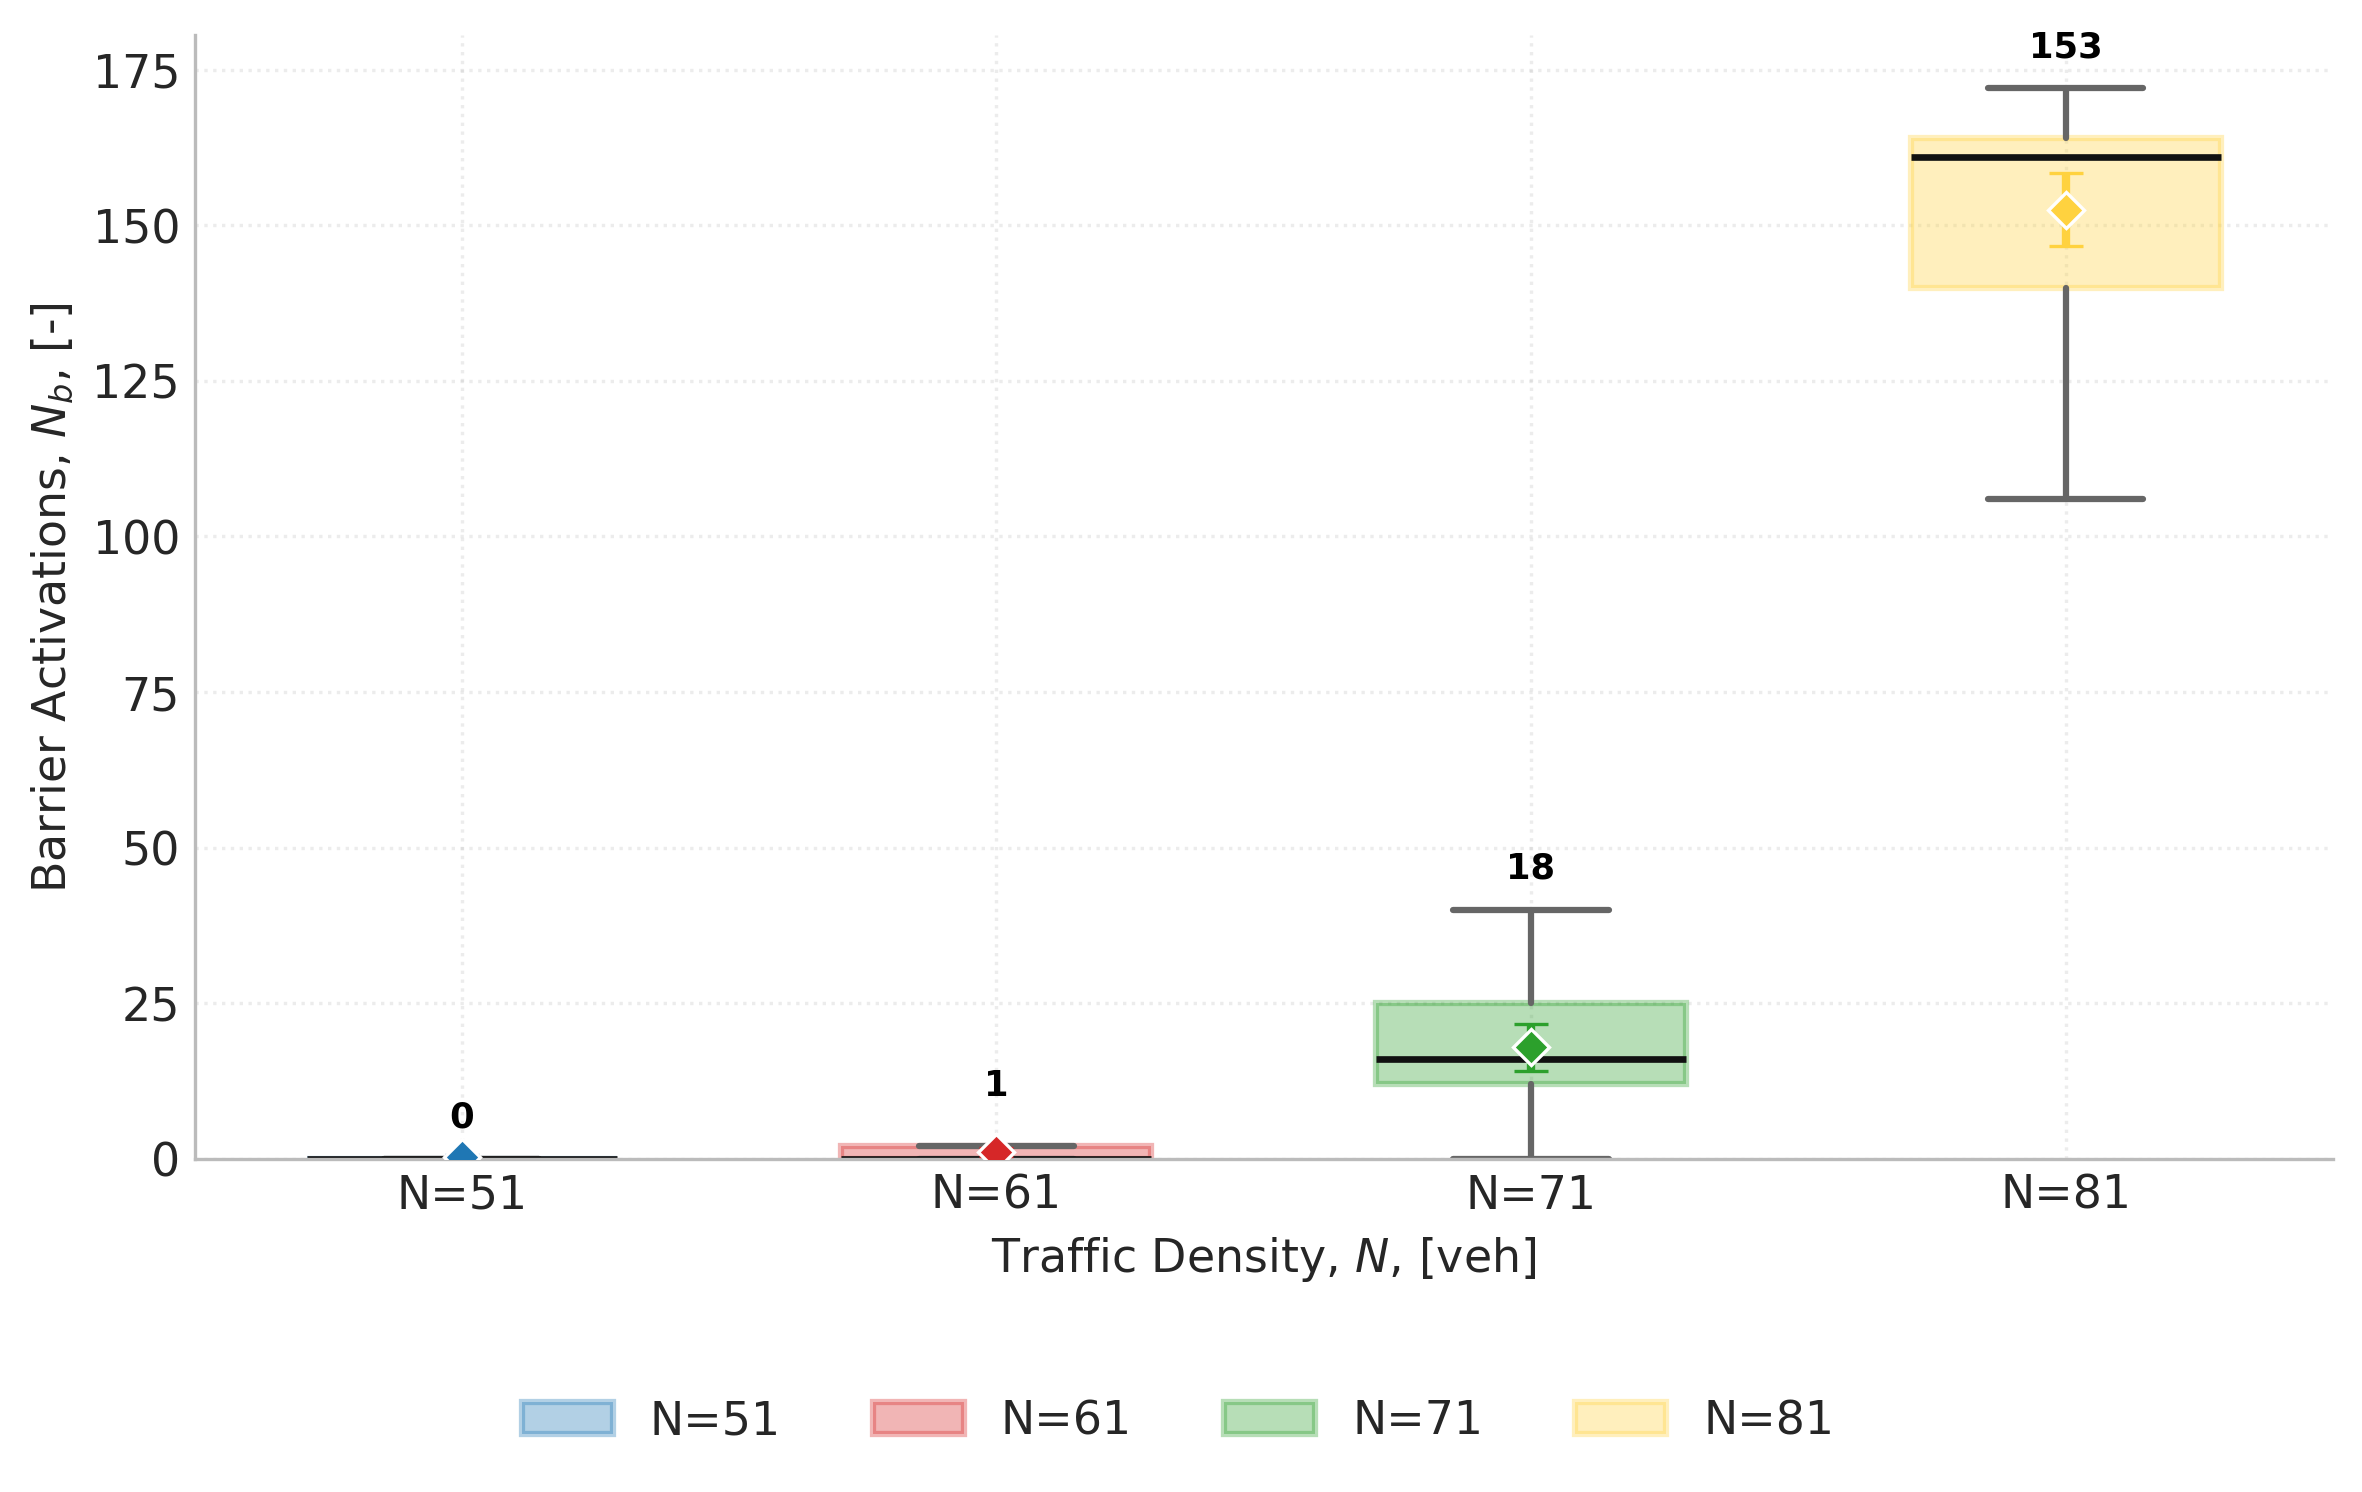
\includegraphics[height=4cm, keepaspectratio]{firings-per-demand.png}
        \caption{Boxplot indicating firings per traffic density \(N\), additional mean and 95\% CI are shown.}
        \label{fig:firings-per-demand}
    \end{subfigure}
    \hfill
    \begin{subfigure}[b]{0.48\textwidth}
        \centering
        % Matching height to ensure perfect alignment
        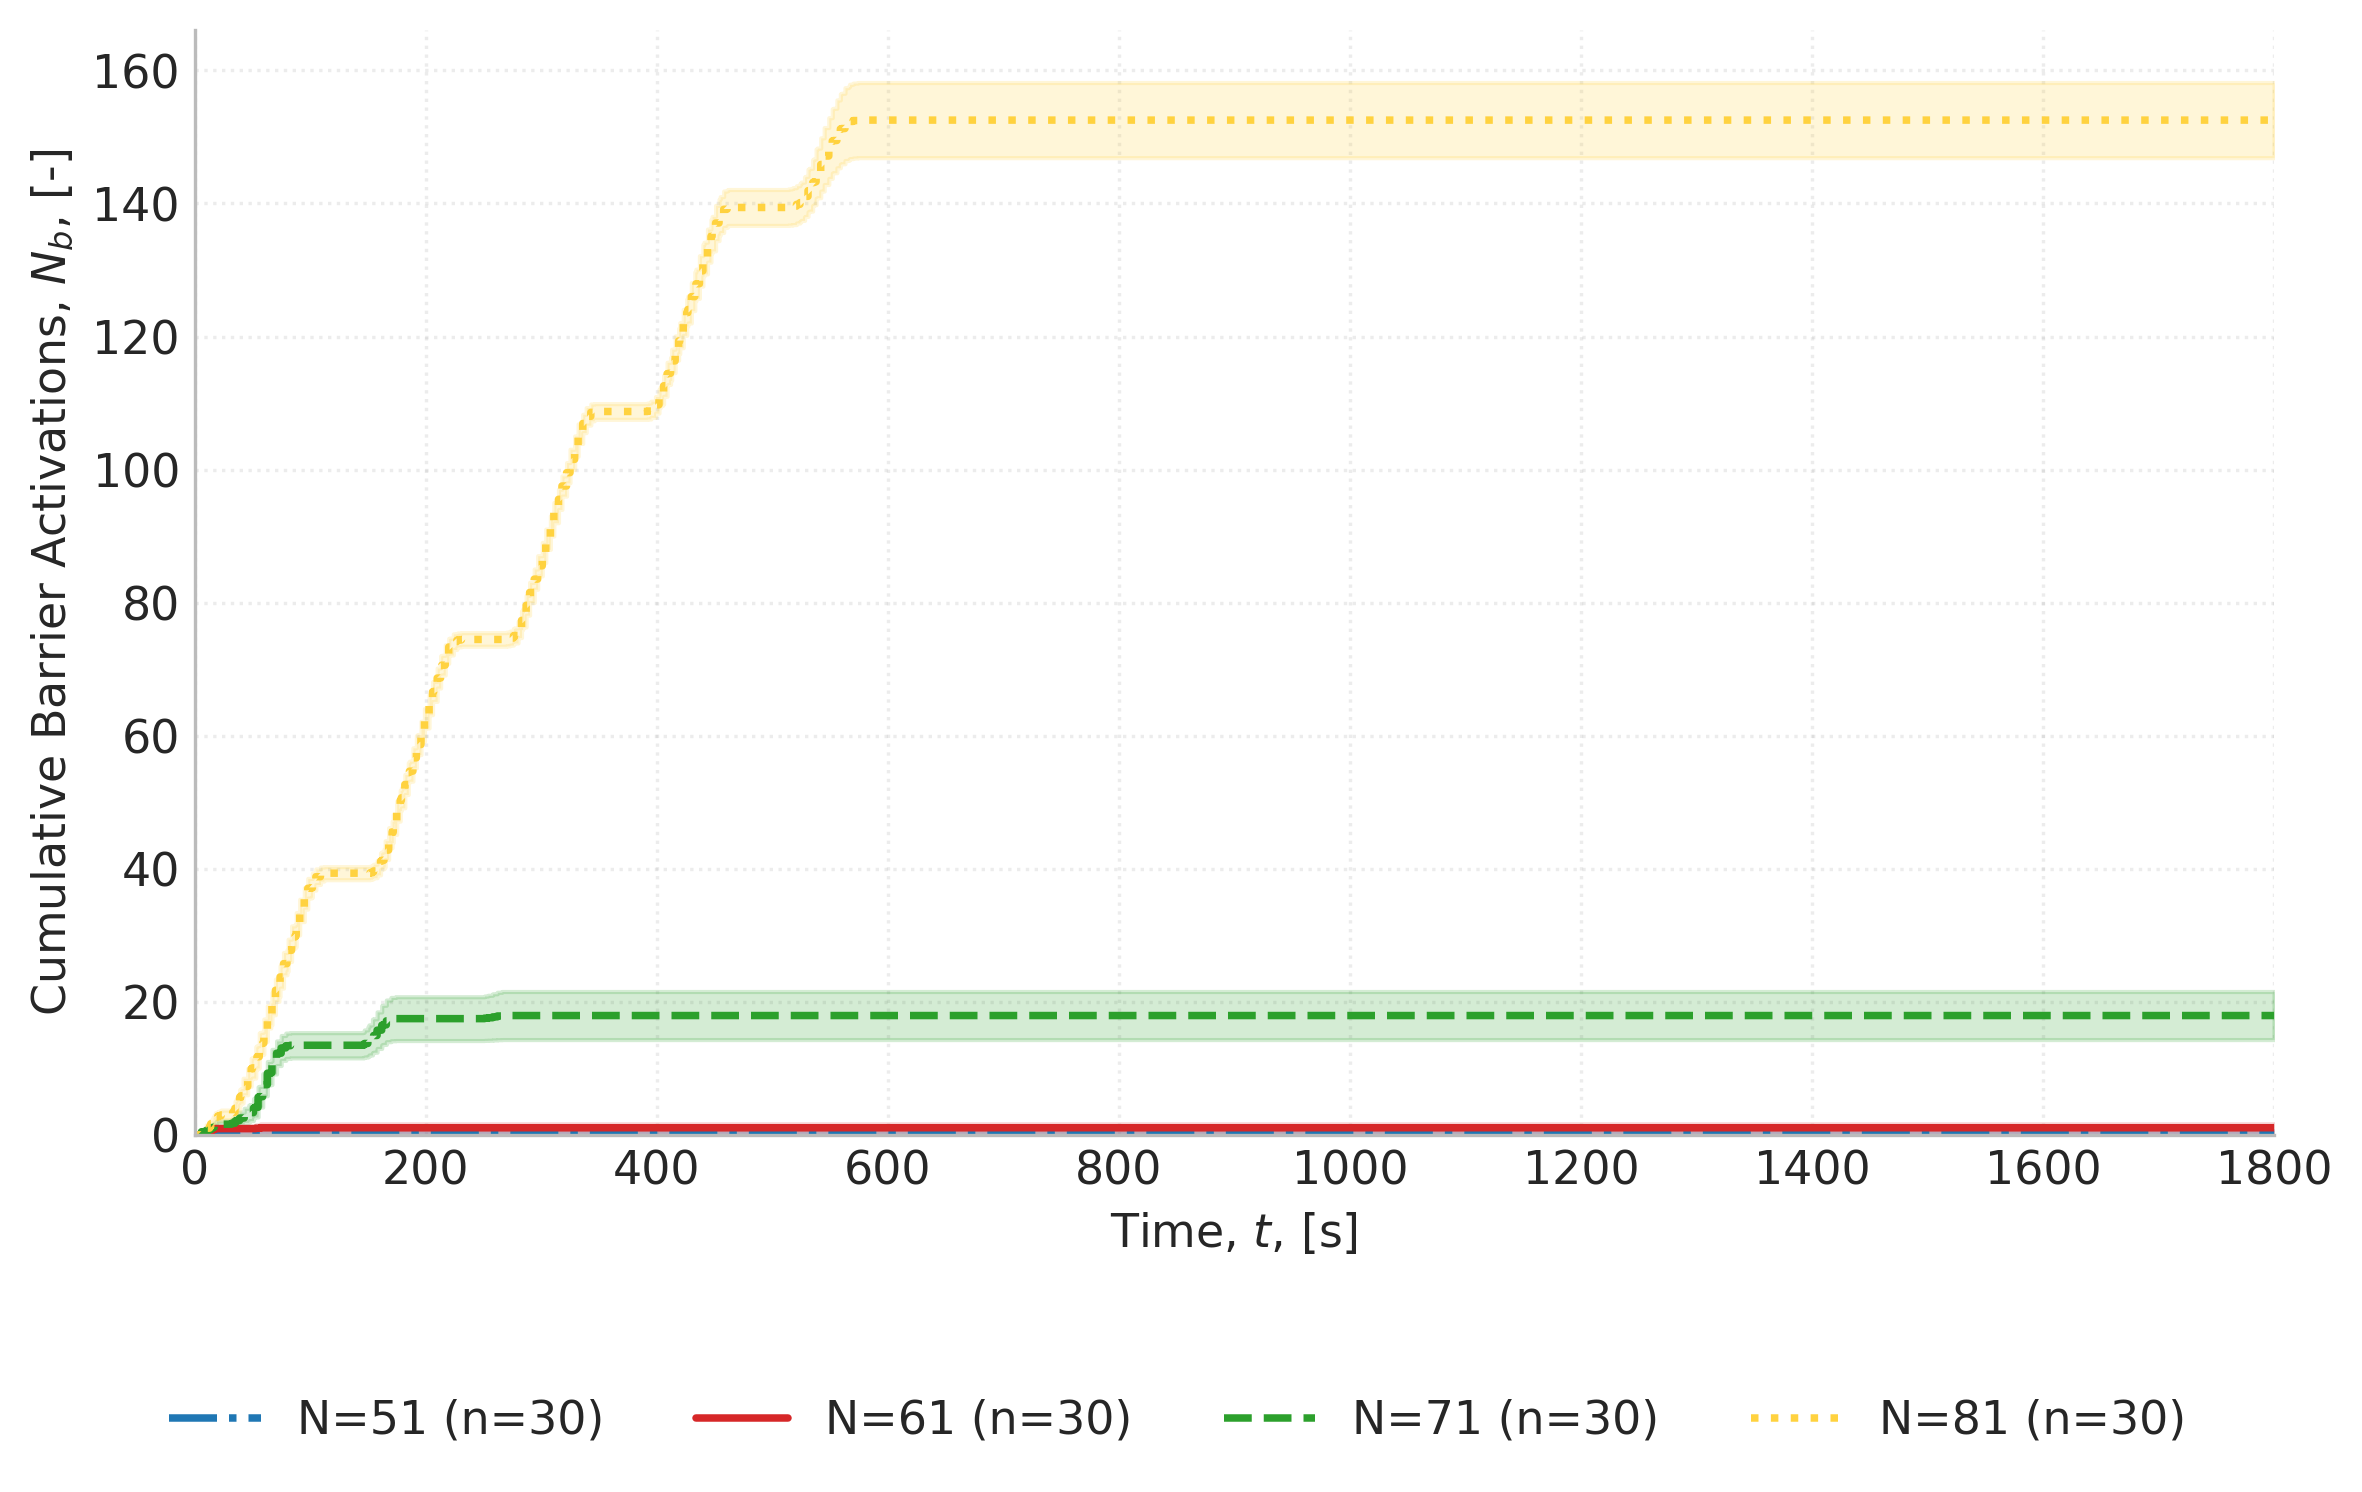
\includegraphics[height=4cm, keepaspectratio]{firings-over-time-all-demands.png}
        \caption{Cumulative firings over time for all traffic densities \(N\), displaying mean and 95\% CI.}
        \label{fig:firings-over-time}
    \end{subfigure}
    
    \caption{Analysis of barrier firings across different vehicle densities \(N = \{51,61,71,81\}\).}
    \label{fig:overall-firings-analysis}
\end{figure}
\subsection{KPI Comparison: Barrier vs. FAS}
This section describes the obtained differences in throughput, delay time, energy consumption, and safety violations from simulations.
 \subsubsection{Throughput}
 Figure~\ref{fig:throughput} displays the mean throughput for each simulation batch, and the error bars highlight the 95\% confidence interval, computed using the t-distribution. First, the figure shows no error bars, indicating that both controllers achieve identical throughput across the various number of runs. Second, the figure shows that the throughput achieved by the barrier controller exhibits a near-linear increase, from 0.36 veh/s at \(N=51\) to 0.57 at \(N=81\). On the other hand, the FAS controller shows a saturation point, around 0.32 veh/s beyond \(N=61\). In general, the barrier controller achieves higher throughput than the FAS controller across all \(N\), with throughput advantages of 34.75\%, 36.09\%, 61.00\% and 72.59\%, at \(N=51, 61, 71,\) and \(81\).   

\subsubsection{Delay Time}
Figure~\ref{fig:delayKPI} displays the mean cumulative delay time across various traffic densities. The figure demonstrates near-zero cumulative delay for the barrier controller across all traffic densities. Conversely, the FAS controller, demonstrates delay across all vehicle counts, ranging from 20000 s at \(N=51\) to 46500 s at \(N=81\). Overall, the barrier controller achieves a maximum decrease in delay time of 98.86\% relative to the FAS controller at \(N=81\).   



\subsubsection{Energy Consumption}
Figure~\ref{fig:energy} illustrates the mean energy consumption, standardized per km traveled. The barrier controller demonstrates near constant energy consumption of 0.077 kWh/km. It should be noted that at \(N=81\), energy consumption was slightly higher, 0.078 kWh/km.
In contrast, the FAS controller shows energy consumption ranging from 0.097 kWh/km at \(N=51\) all the way to 0.14 kWh/km at \(N=81\). Overall,  the barrier achieves energy reductions of 20.12\%, 22.85\%, 39.97\%, and 44.81\% at \(N=51, 61, 71,\) and \(81\).  


\subsubsection{Safety Violations}
Figure~\ref{fig:safetycounting} displays the mean safety violations per traffic density. Both controllers show zero safety violations at \(N=\{51,61\}\). Whereas, the FAS controller continues with near-zero violations at \(N=\{71,81\}\), the barrier controller records  1.9±0.82 violations per run at \(N=71\), and 21.13±1.69 violations per run at \(N=81\). Despite these counted safety violations, figure~\ref{fig:safety-violations-time} shows that the violations only occur during the non steady-state phase. Once steady-state is reached, no further violations occur. 

\begin{figure}[H]
    \centering
    % Row 1
    \begin{subfigure}[b]{0.48\textwidth}
        \centering
        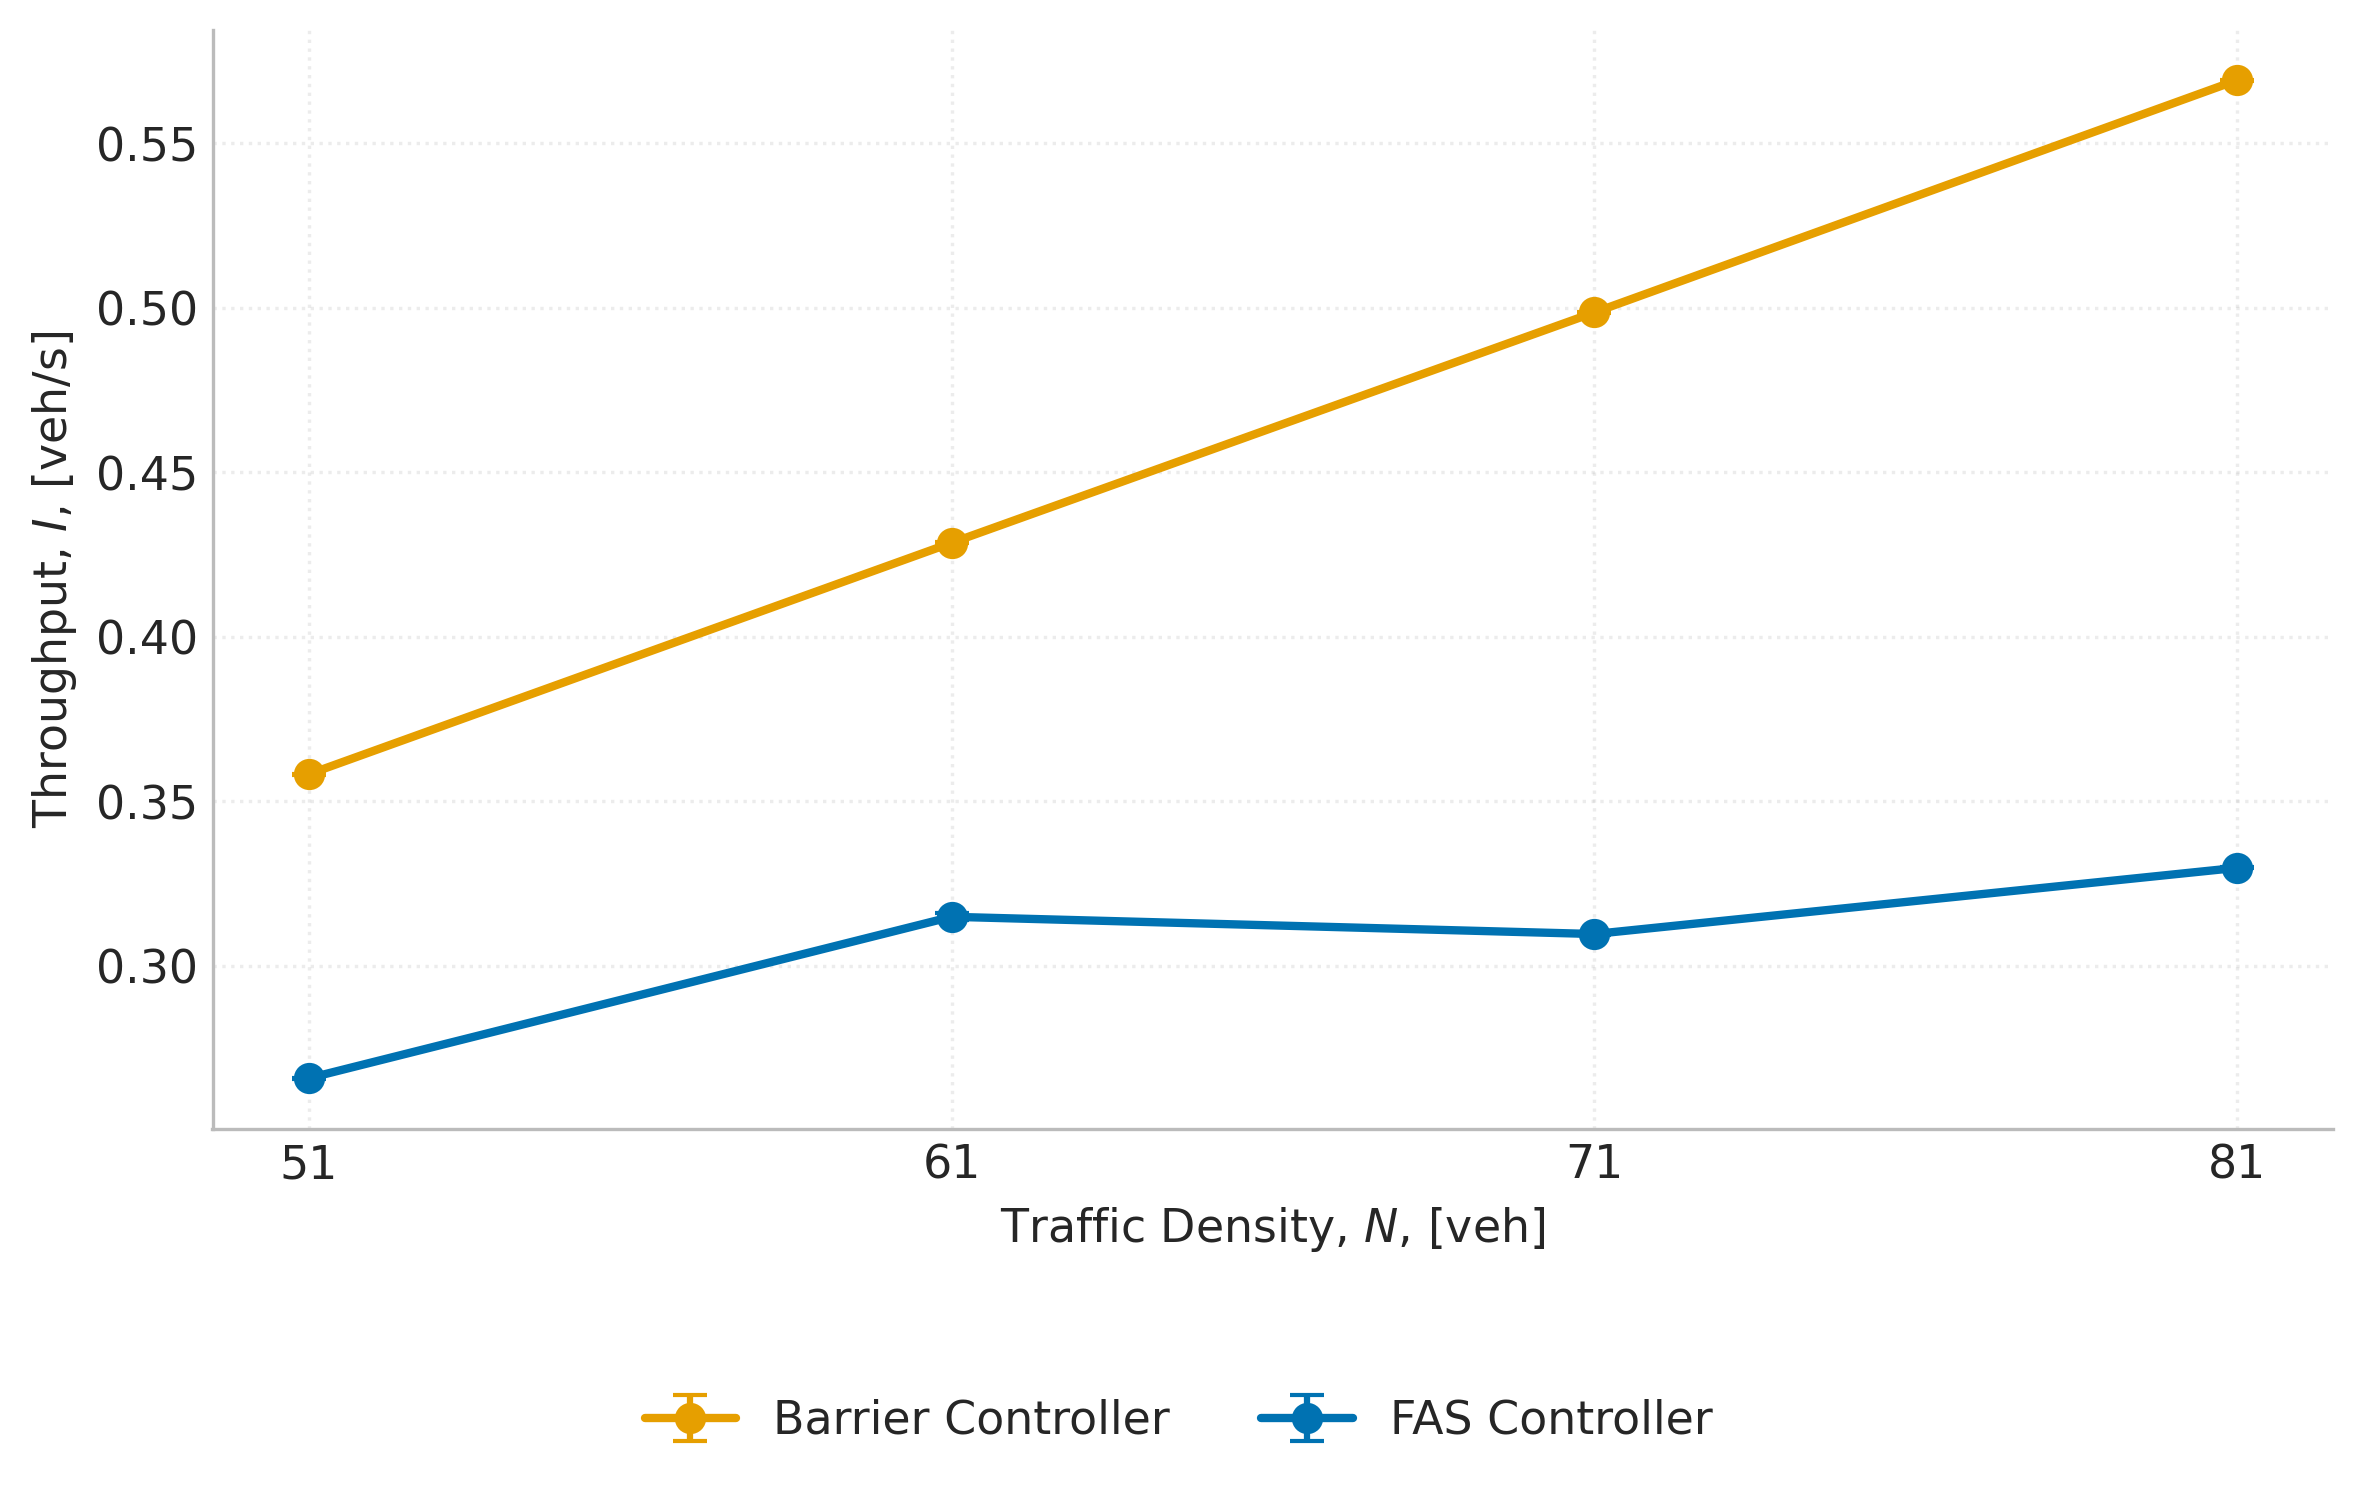
\includegraphics[width=\textwidth]{throughput-veh-s.png}
        \caption{Throughput}
        \label{fig:throughput}
    \end{subfigure}
    \hfill
    \begin{subfigure}[b]{0.48\textwidth}
        \centering
        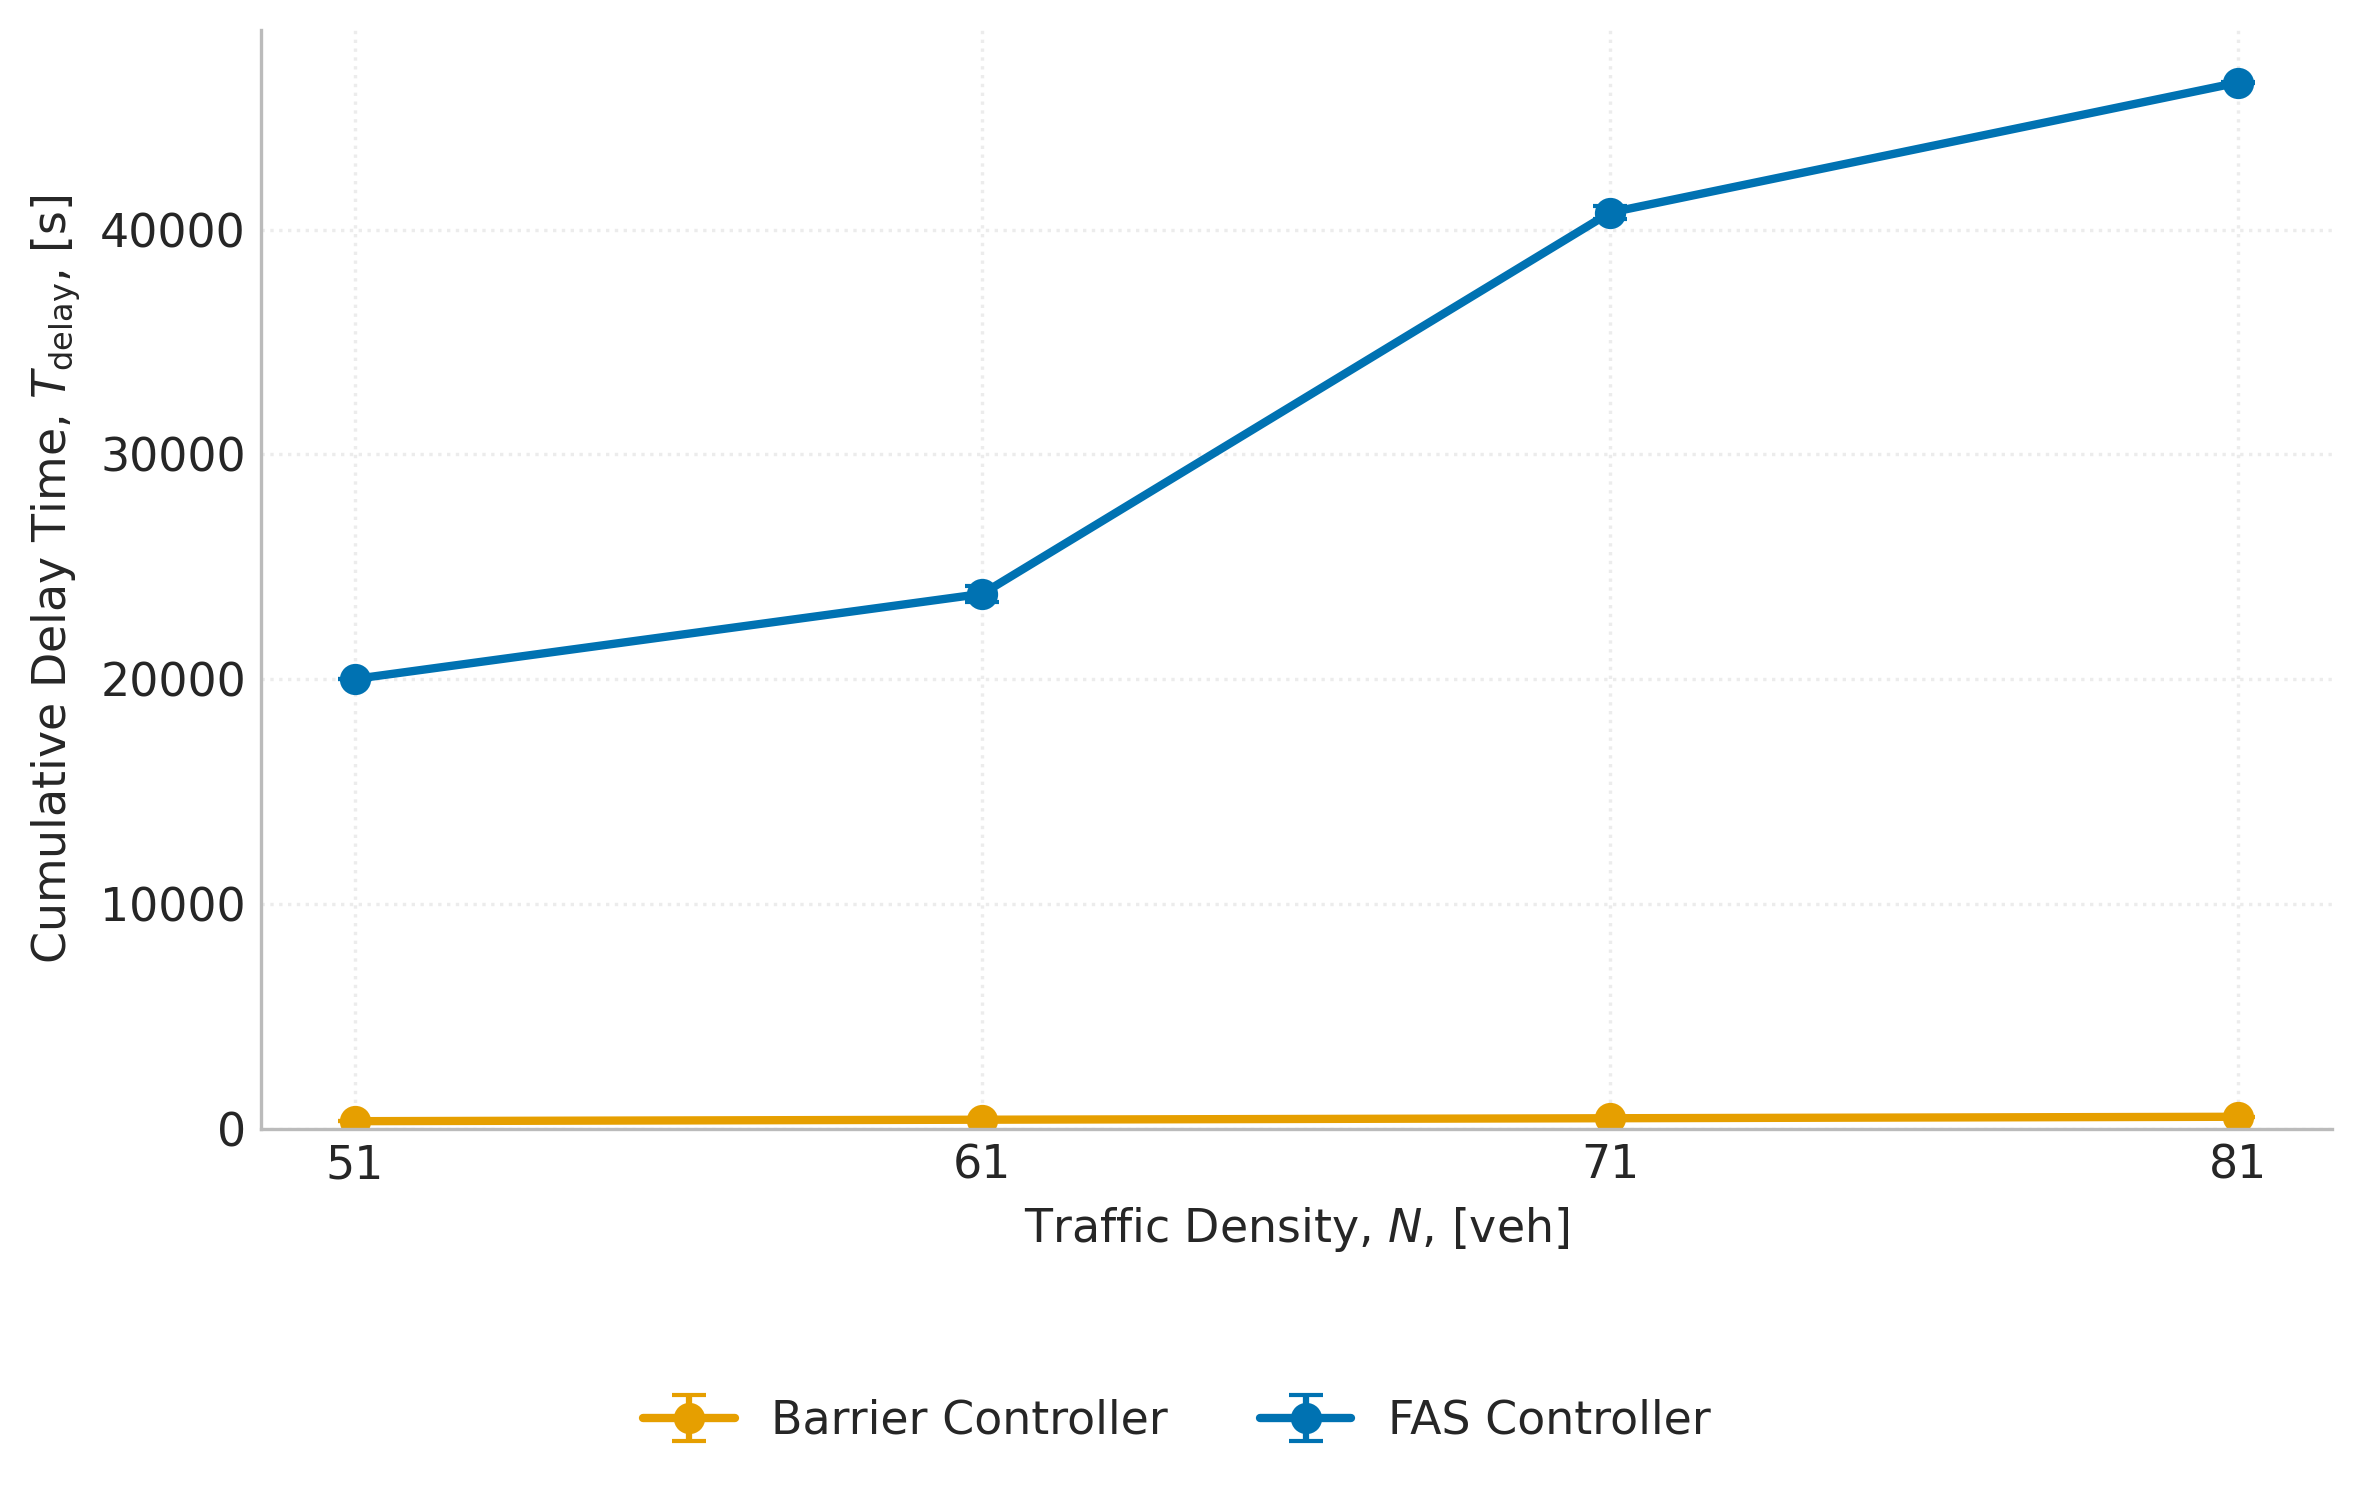
\includegraphics[width=\textwidth]{delay-s.png}
        \caption{Delay Time}
        \label{fig:delayKPI}
    \end{subfigure}
    
    \vspace{10pt} % Adds vertical spacing between the rows
    
    % Row 2
    \begin{subfigure}[b]{0.48\textwidth}
        \centering
        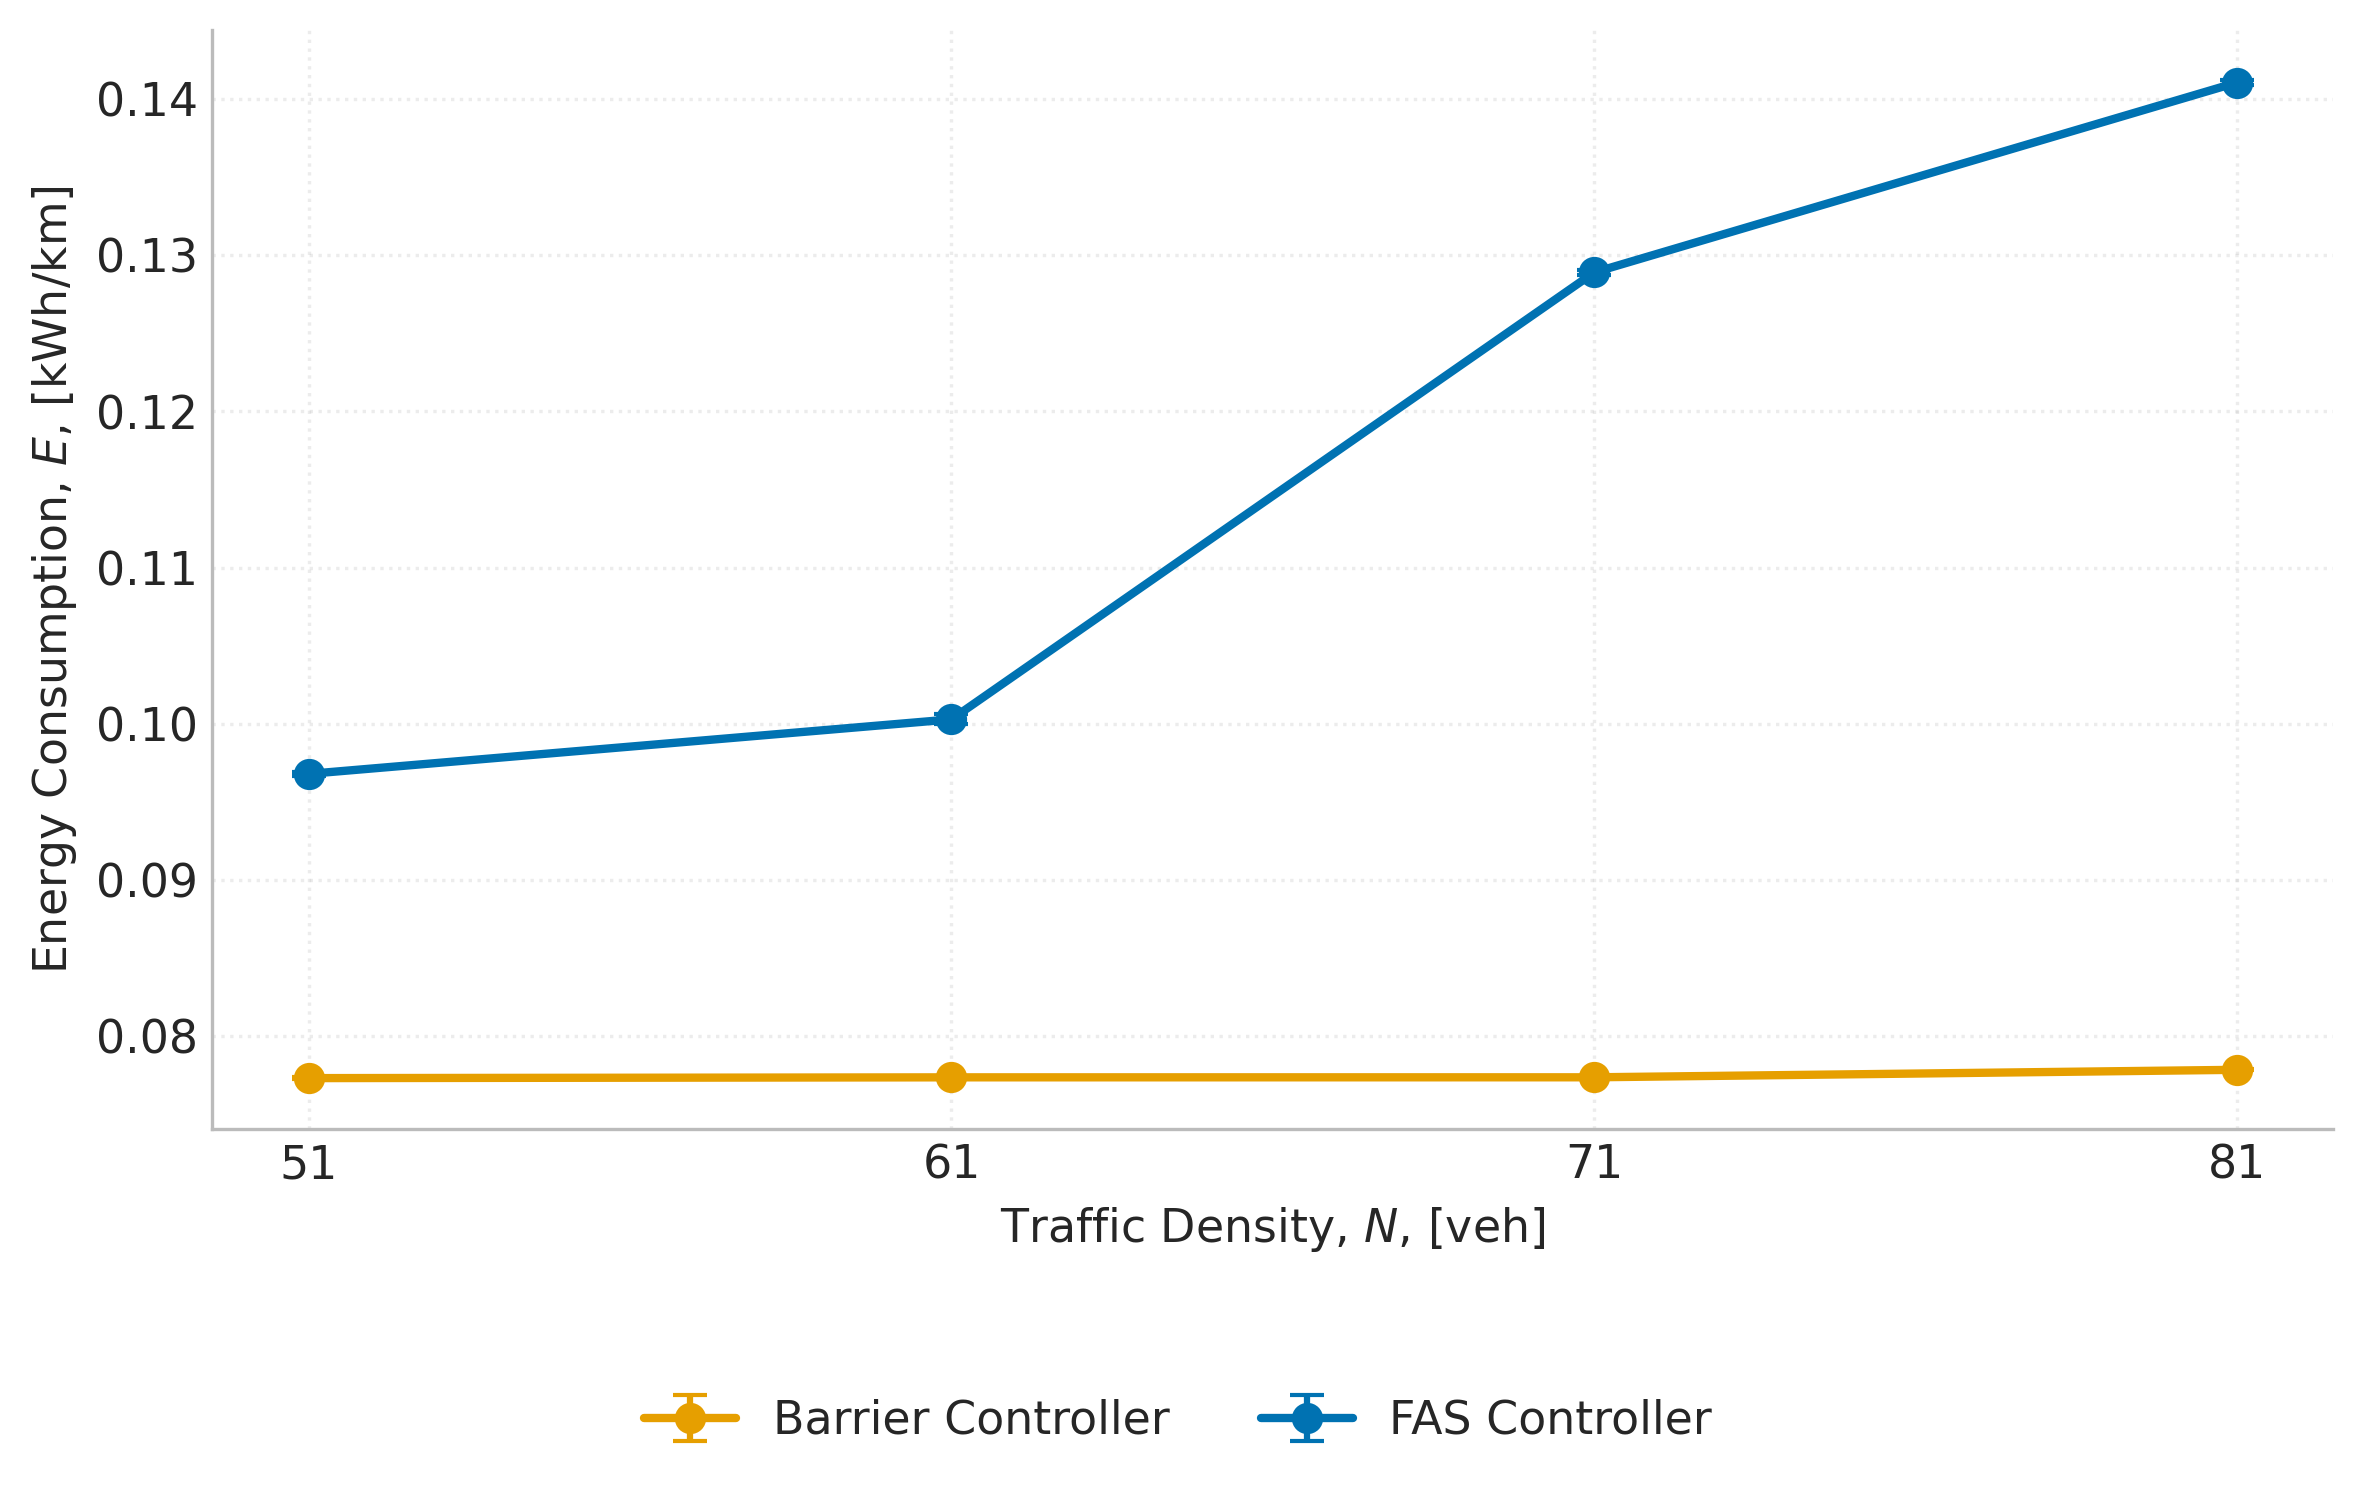
\includegraphics[width=\textwidth]{energy-kwh-per-km.png}
        \caption{Energy Consumption}
        \label{fig:energy}
    \end{subfigure}
    \hfill
    \begin{subfigure}[b]{0.48\textwidth}
        \centering
        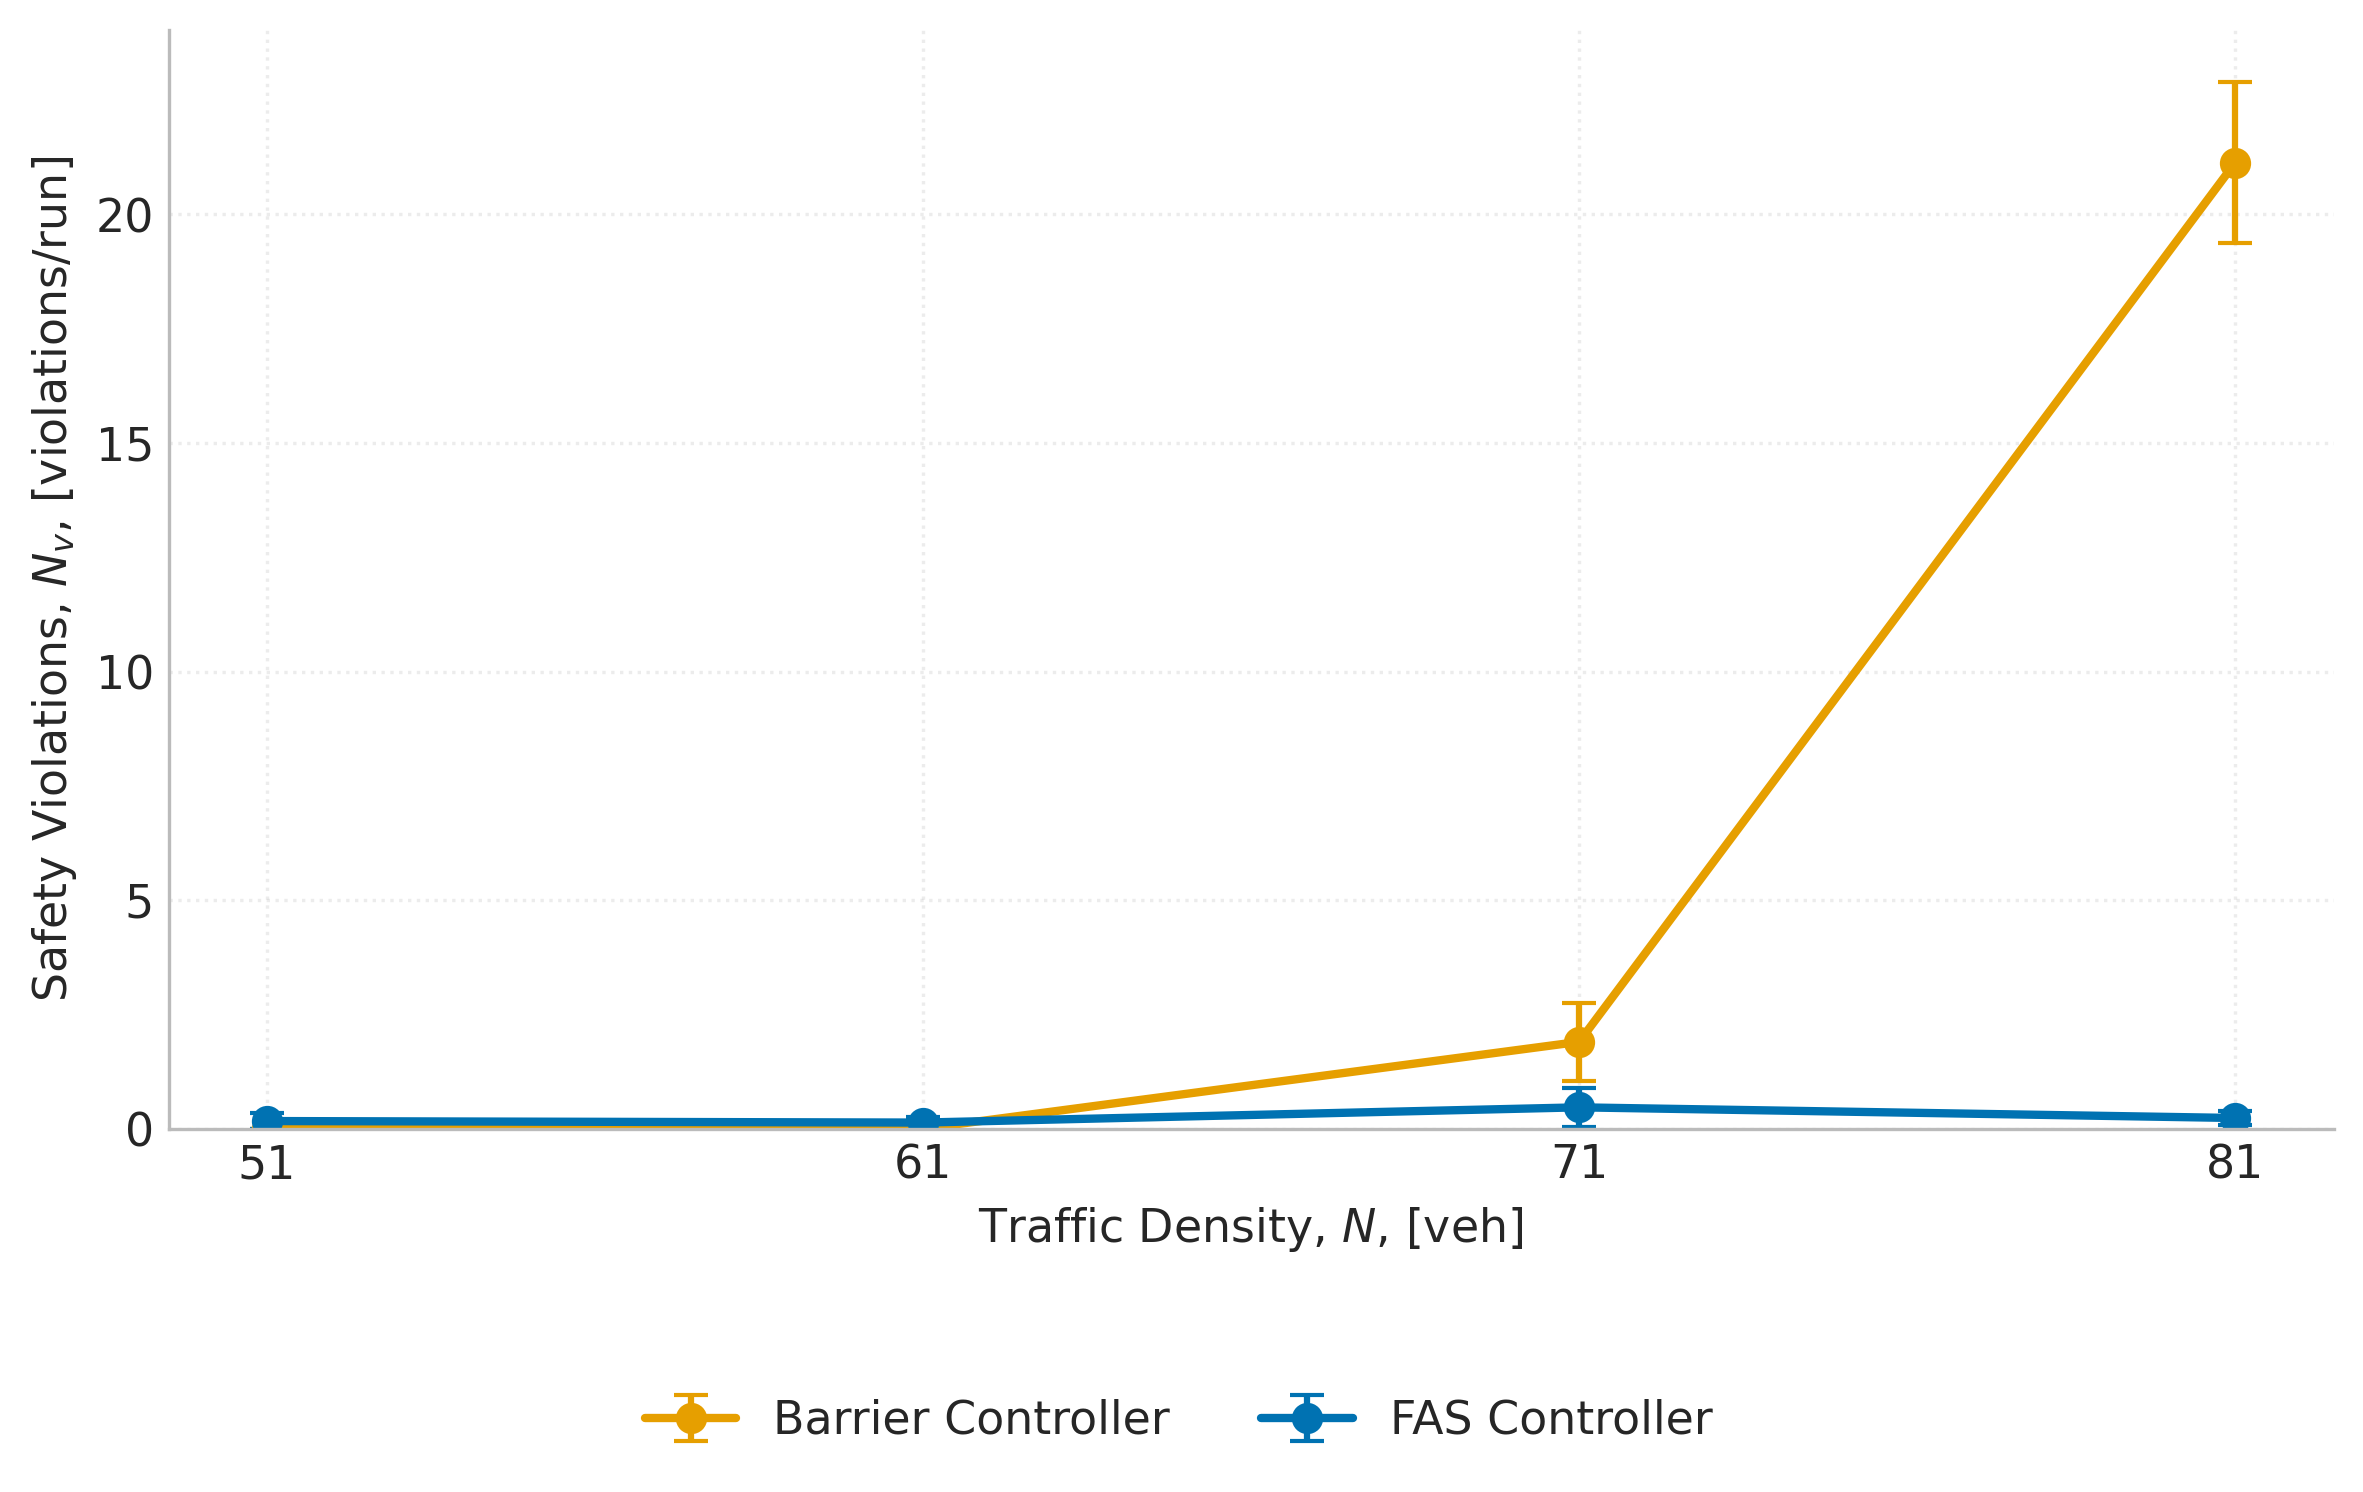
\includegraphics[width=\textwidth]{safety-violations-count.png}
        \caption{Safety Violations}
        \label{fig:safetycounting}
    \end{subfigure}
    
    \caption{Comparison of key performance indicators across traffic densities $N=\{51,61,71,81\}$, showing mean and 95\% CI.}
    \label{fig:kpi-four-metrics}
\end{figure}
\begin{figure}[H]
    \centering
    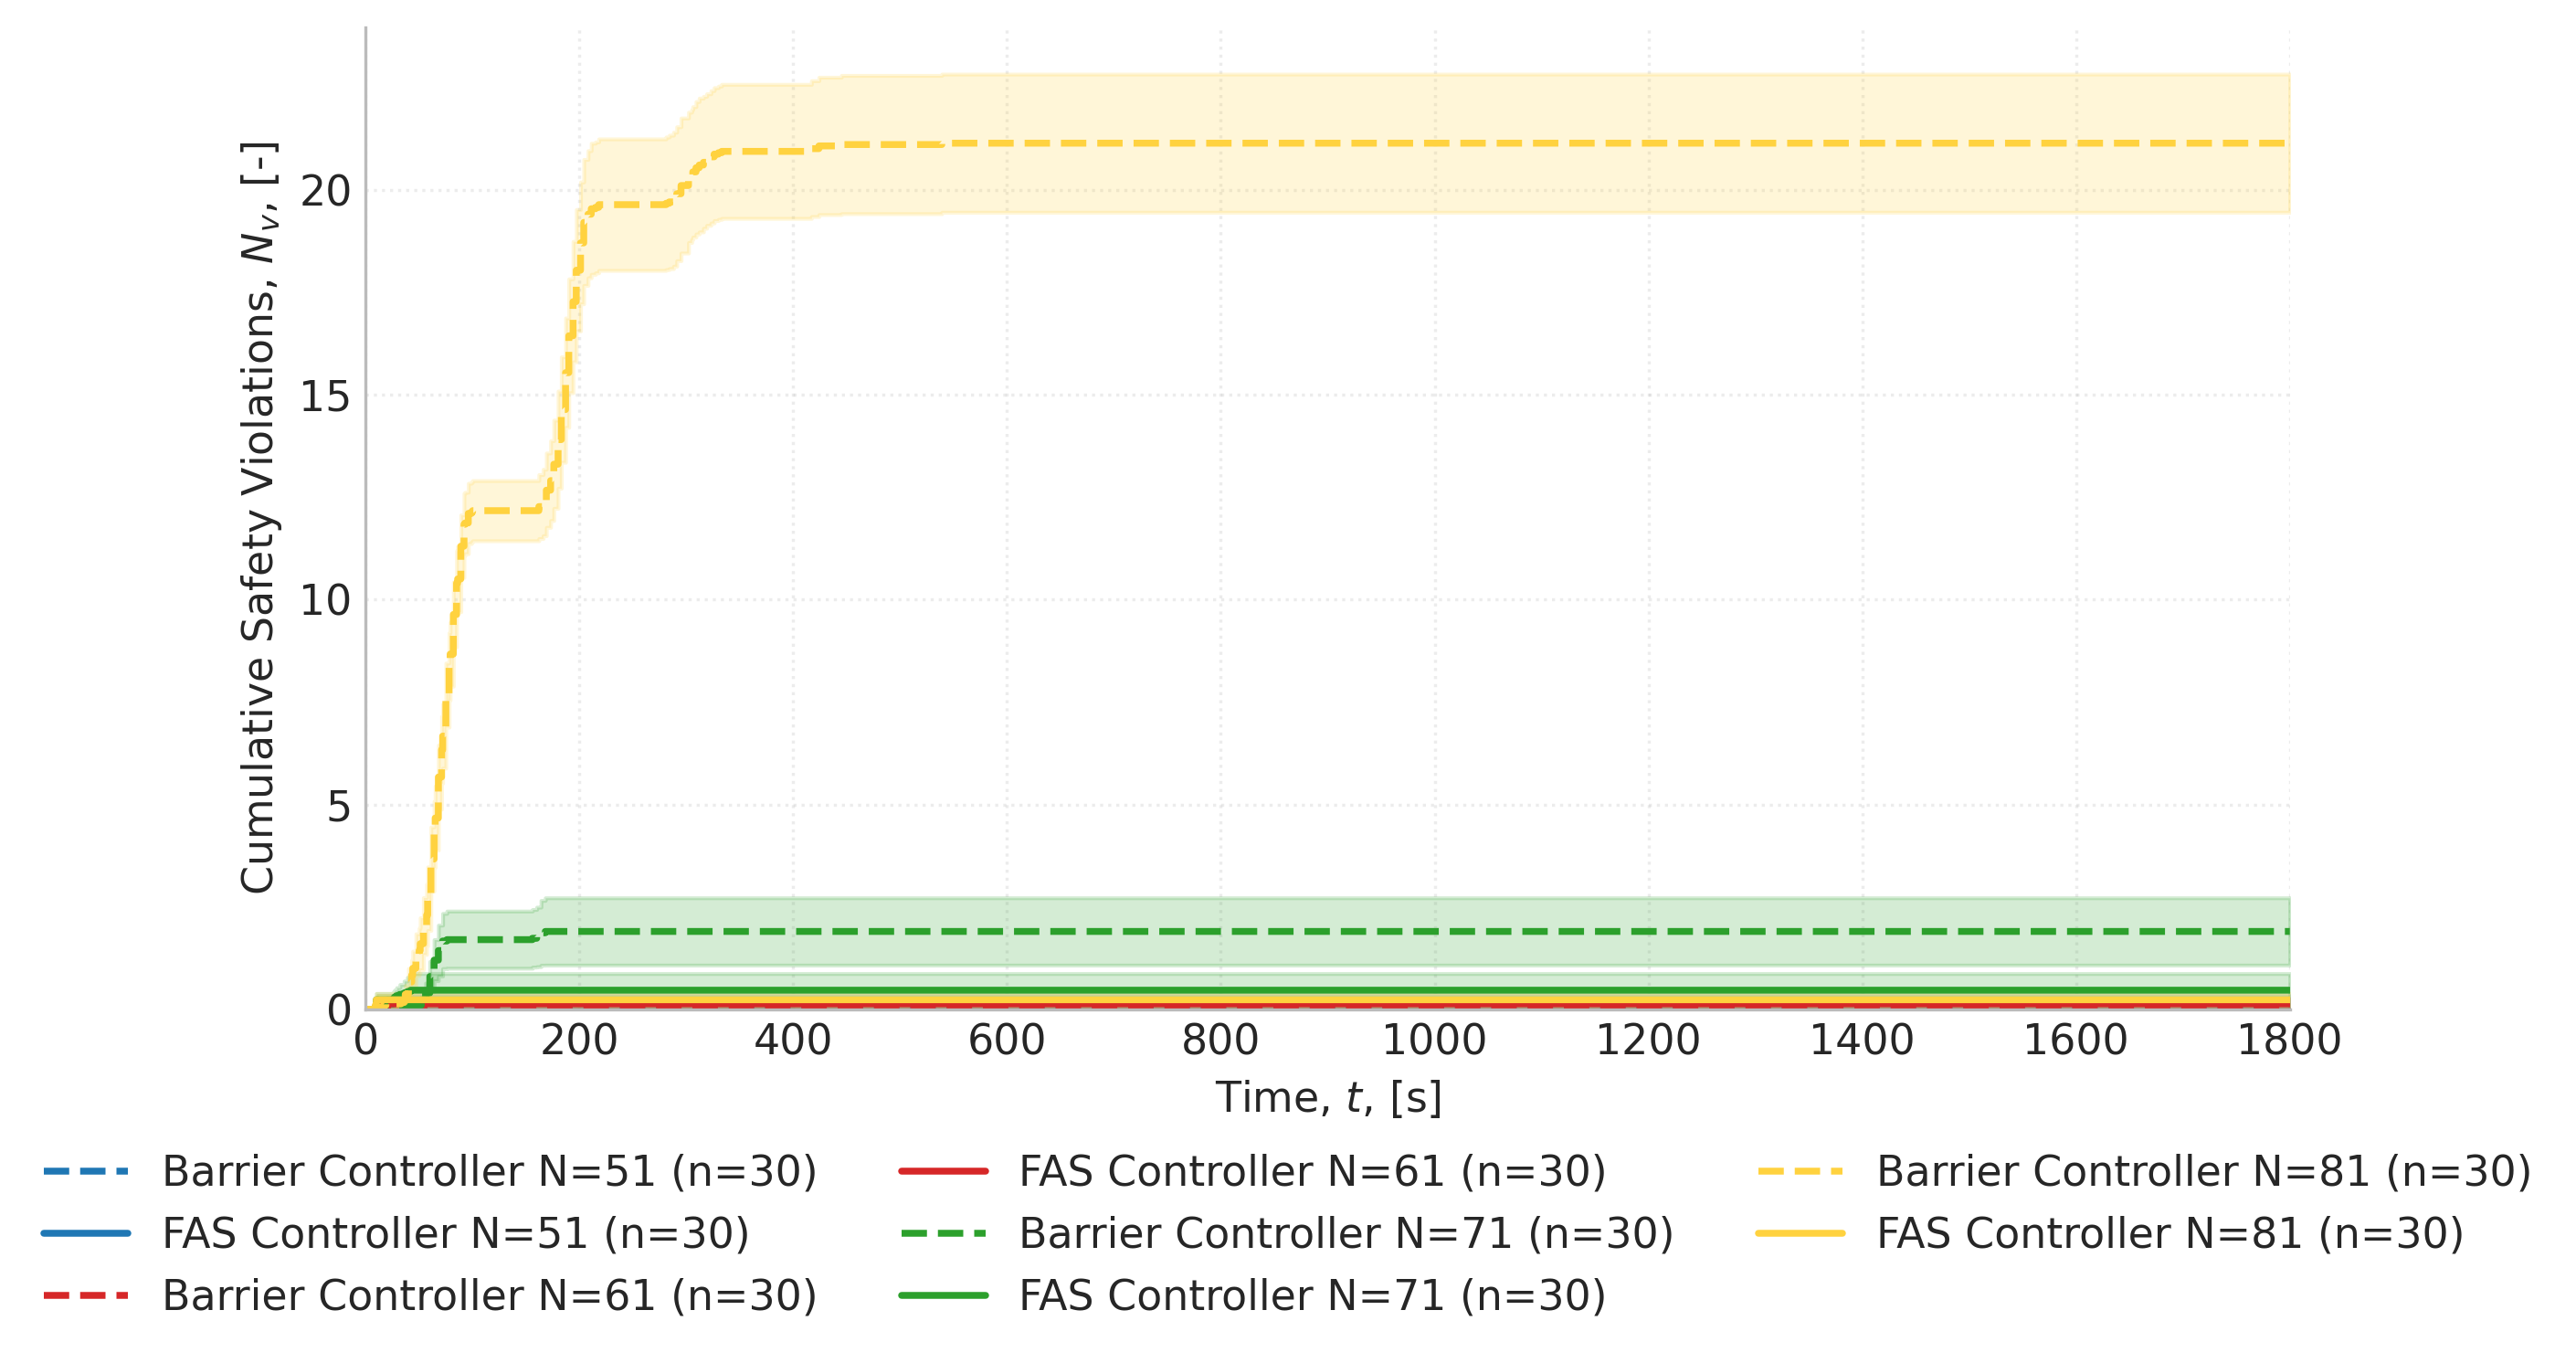
\includegraphics[width=\linewidth]{safety-violations-over-time.png}
    \caption{Cumulative safety violations over time across traffic densities \(N\ =\{51,61,71,81\}\), showing mean and 95\% CI.}
    \label{fig:safety-violations-time}
\end{figure}
\newpage
\section{Discussion}
\label{Discussion}
This section interprets the results, connects them to the underlying mechanisms, and discusses limitations of the study.

\subsection{Platoon Formation Drives Performance Gains}
The throughput, delay time, and energy consumption results all arise from the same root cause. The barrier controller converges the vehicles into a platoon, which is spaced in a manner that allows vehicles to cross the conflict point continuously, without mandatory stops. On the other hand, the FAS controller imposes idle time through its phase cycles. Despite its adaptive setup, the adaptive extension saturates beyond \(N=61\), resulting in the green time being extended to the maximum green time across all cycles, degrading the adaptive traffic light to a fixed-cycle traffic light. This difference explains why the throughput of the barrier controller scales near-linearly with vehicle count, while  the FAS controller saturates at approximately 0.32 veh/s beyond \(N=61\). 
\\\\
Delay time and energy consumption results follow from the continuous flow, which results in vehicles driving at target speed throughout the run, resulting in small deviations in lap time and the motor operating at low torque, in a high efficiency region. Conversely, the FAS controller does the opposite by imposing stop-and-go behavior. The stops result in decelerations, followed by rapid accelerations during the go, which drive the motor into operating at high-torque, in the low efficiency region. In addition, driving in queues forces the motor into driving at low torque and shaft speed, which is a second region of poor efficiency. Both effects have a greater impact at higher vehicle counts, since the traffic light already performs at maximum capacity, therefore the additional vehicles add directly to the queue. This explains why the gap in energy widens at \(N=71\) and \(N=81\), rather than scaling linearly. The energy reduction of maximum 44.81\% confirms that stop-and-go behavior is a primary driver of EV energy consumption at intersections.
\\\\
Safety is the only performance indicator showing opposite behavior. At low vehicle counts both controllers record zero violations. Whereas from \(N=71\), the barrier controller records safety violations during the phase before the continuous flow platoon is formed. This highlights a key limitation of the barrier controller setup: either the activation distance is too small, the cap of ±7 km/h is to small, or the barrier gain is set to gentle to separate vehicles with small inter-vehicle spacing. The FAS controller avoids this by having mutually exclusive phases which avoid simultaneous arrival. It is important to note, that violations are completely eliminated once steady state is reached, indicating that the barrier law itself is capable of safe operation. The violations reflect the initial spawn noise and the barrier corrections, rather than a fundamental barrier shortcoming.


\subsection{Simulation Limitations}
Although promising results have been found, this study also has limitations. First, the figure-eight track is a highly controlled environment, with a single conflict point, constant vehicle flow, no steering at the intersection, and absence of pedestrians or emergency vehicles. Therefore, performance at a multi-lane intersection with stochastic arrivals, pedestrians and emergency vehicles, and steering may differ. Second, the energy model relies on approximated efficiency maps from other literature, rather than manufacturer efficiency maps. The model is also subjected to severe assumptions, due to absence of data. Since both controllers are subjected to identical assumptions, the difference remains valid, but the produced outcomes should be interpreted with caution since they differ from actual values. Third, the barrier controller was only compared against a FAS controller based on Dutch standards according to \textcite{wilson2014handboek}. The book was published in 2014, so it is likely that more advanced controllers exist, which might close some of the performance gaps. Fourth, the simulation assumes that each vehicle is capable of perfectly estimating its own distance and the distance of the conflicting vehicle to the conflict point using onboard sensors. In practice, sensors are subjected to noise and estimation errors, which could reduce the accuracy of the distance measurement, which might affect performance and safety of the barrier controller.

\newpage
\section{Conclusion}
\label{Conclusion}
This thesis evaluated a barrier control algorithm against an FAS controller on a closed-loop figure-eight track across four traffic densities under varying initial conditions, using CARLA, a physics based simulator. Both evaluated controllers were subjected to identical simulation conditions, ensuring that differences in controller performance in terms of KPIs, could be solely attributed to the controllers. The results show that the barrier controller outperforms the FAS controller in throughput, delay, and energy consumption, across all traffic densities. The results can be attributed to the formed steady-state platoon, which allows continuous crossing of the intersection, eliminating idle time and stop-and-go behavior, which are in fact present during simulations of the FAS controller. The energy consumption reduction highlighted that stop-and-go behavior at intersections is a driver of increased energy consumption of electric vehicles. 
These performance gains, however, come at a safety cost at higher traffic densities, making safety the only KPI where the FAS controller performs better. Nevertheless, the violations only occurred during the transient phase, which is the phase before the steady-state platoon is formed. After the platoon was formed, the barrier showed no violations, indicating that the barrier controller is capable of safe operation, but needs parameter tuning for higher traffic densities. 
\\\\
Future research could improve and extend this project in five directions. First, research should focus on the adjustment of the barrier controller parameters to eliminate safety violations. This tuning can be in terms of either more aggressive fixed values or as an adaptive function based on traffic density. Second, future research should extend to a double-intersection, to assess if the barrier controller is scalable beyond the single-intersection. Third, the performance of the barrier controller should be evaluated under sensor noise, since the simulation assumes perfect distance estimation, whereas sensors are subject to measurement noise, which may affect safety and overall performance of the barrier controller. Fourth, for actual energy performance the energy model should be made more accurate by removing the stated assumptions. 
Fifth, the barrier control algorithm should be evaluated in a controlled laboratory or in the real world. 

\newpage
\setlength{\bibitemsep}{0.5\baselineskip}
\printbibliography[title={References}, heading=bibintoc]
\newpage
\section*{Appendix}
\addcontentsline{toc}{section}{Appendix}
\subsection*{Appendix A}
\addcontentsline{toc}{subsection}{Appendix A}

In the preparation of this report, generative artificial intelligence (AI) tools were used in a
supportive role. Specifically, Claude Sonnet 4.6 (Anthropic) was consulted to assist with language
refinement, structural suggestions, and clarification of technical explanations. The tool was used to improve readability, coherence, and academic tone, as well as to support the
drafting and revision of text sections, and debugging of coding tasks.\\\\
No AI tools were used to generate original research data, perform analyses, make design
decisions, or draw conclusions. All technical content, interpretations, results, and conclusions presented in this report are the sole responsibility of the author. All sources were independently selected, verified, and cited by the author in accordance with
academic standards.\\\\
The use of generative AI was limited to support functions and was conducted in line with
the University of Groningen’s guidelines on the responsible use of artificial intelligence in
education and research.
\subsection*{Appendix B}
\addcontentsline{toc}{subsection}{Appendix B}

\begin{table}[H]
\caption{Simulation Configuration and Controller Parameters}
\centering
\begin{tabular}{lll}
\toprule
\textbf{Group} & \textbf{Parameter} & \textbf{Value} \\
\midrule
Longitudinal Controller & $K_p$ & 0.5 \\
Longitudinal Controller & $K_I$ & 0.25 \\
Longitudinal Controller & $K_d$ & 0.02 \\
\midrule
Headway Controller & $K_p$ & 3.5 \\
Headway Controller & $K_d$ & 1.0 \\
Headway Controller & Headway Alpha ($\alpha_\text{headway}$) & 0.9 \\

\midrule
Barrier Controller & $K_{\text{barrier}}$ & 25.0 \\
Barrier Controller & Activation Distance & 10 m \\
Barrier Controller & Approach Window & 20 m \\
\midrule
FAS Controller & Stop Line Distance & 12.0 m \\
FAS Controller  & Approach Window (\(d_\text{approach}\)) & 50.0 m \\
FAS Controller & Reaction Time ($t_r$) & 1.0 s \\
FAS Controller  & Max Deceleration ($a_{off}$) & 2.5 m/s$^2$ \\
FAS Controller & Queue Start-up Lost Time ($t_{\text{away}}$) & 2.0 s \\
FAS Controller & Discharge Headway Peak ($t_{\text{follow}}$) & 2.5 s/vehicle \\
FAS Controller & Maximum yellow time ($t_{\text{ymax}}$) & 1.0 s \\
FAS Controller & Maximum allowed time gap($t_{\text{gap}}$) & 4.0 s \\
FAS Controller & Average Vehicle Length ($L_{\text{veh}}$) & 5.0 m \\
FAS Controller & Buffer Gap Between Cars ($d_{\text{gap}}$) & 1.0 m \\
FAS Controller & Stop-line to Upstream Loop Distance ($d$) & 30.0 m \\
FAS Controller & Request Loop Length ($L_{\text{request}}$) & 10.0 m \\
FAS Controller & Discharge Loop  Length ($L_{\text{loop}}$) & 5.0 m \\
FAS Controller & yellow-time (\(t_y\)) & 4 s \\
FAS Controller & minimum green-time (\(t_\text{gmin}\)) & 12 s \\
FAS Controller & maximum green-time (\(t_\text{gmax}\)) & 45 s \\
FAS Controller & gap-out threshold (\(t_\text{go}\)) & 3.4 s \\
\midrule
Energy Consumption & Acceleration Alpha ($\alpha_\text{acceleration}$) & 0.5 \\
\midrule
Key Performance Indicator & Safety violation distance  & 5 m\\
Key Performance Indicator & Free flow lap time (\(t_\text{ideal}\)) & 281.78s\\
\bottomrule
\end{tabular}
\label{tab:simulation_parameters}
\end{table}
\end{document}
